Figures~\ref{fig:pt4lunf}-\ref{fig:dphiunf} show the predicted reconstructed and particle level yields, as well as the efficiency, fiducial purity (equivalent to the diagonal elements of the migration matrices) and fiducial fraction for each bin of each distribution, after the pre-unfolding is applied.  

When selecting the binning, it was required that all bins contain at least 10 predicted events passing the reconstruction-level selection, and that the fiducial purity was at least 60$\%$. Bins predicted to contain between 10 and 20 events passing the reconstruction-level selection were required to have a more stringent fiducial purity of 80$\%$, to avoid problems interpreting the unfolded results. Note, that the yields are normalised by bin width to show clearly that the number of events per bin satisfy the criteria we required, but this can lead to the distributions looking jumpy. When normalised to events per GeV the curves are smooth, as expected. 

\begin{figure}[htb]
  \centering 
  \subfigure{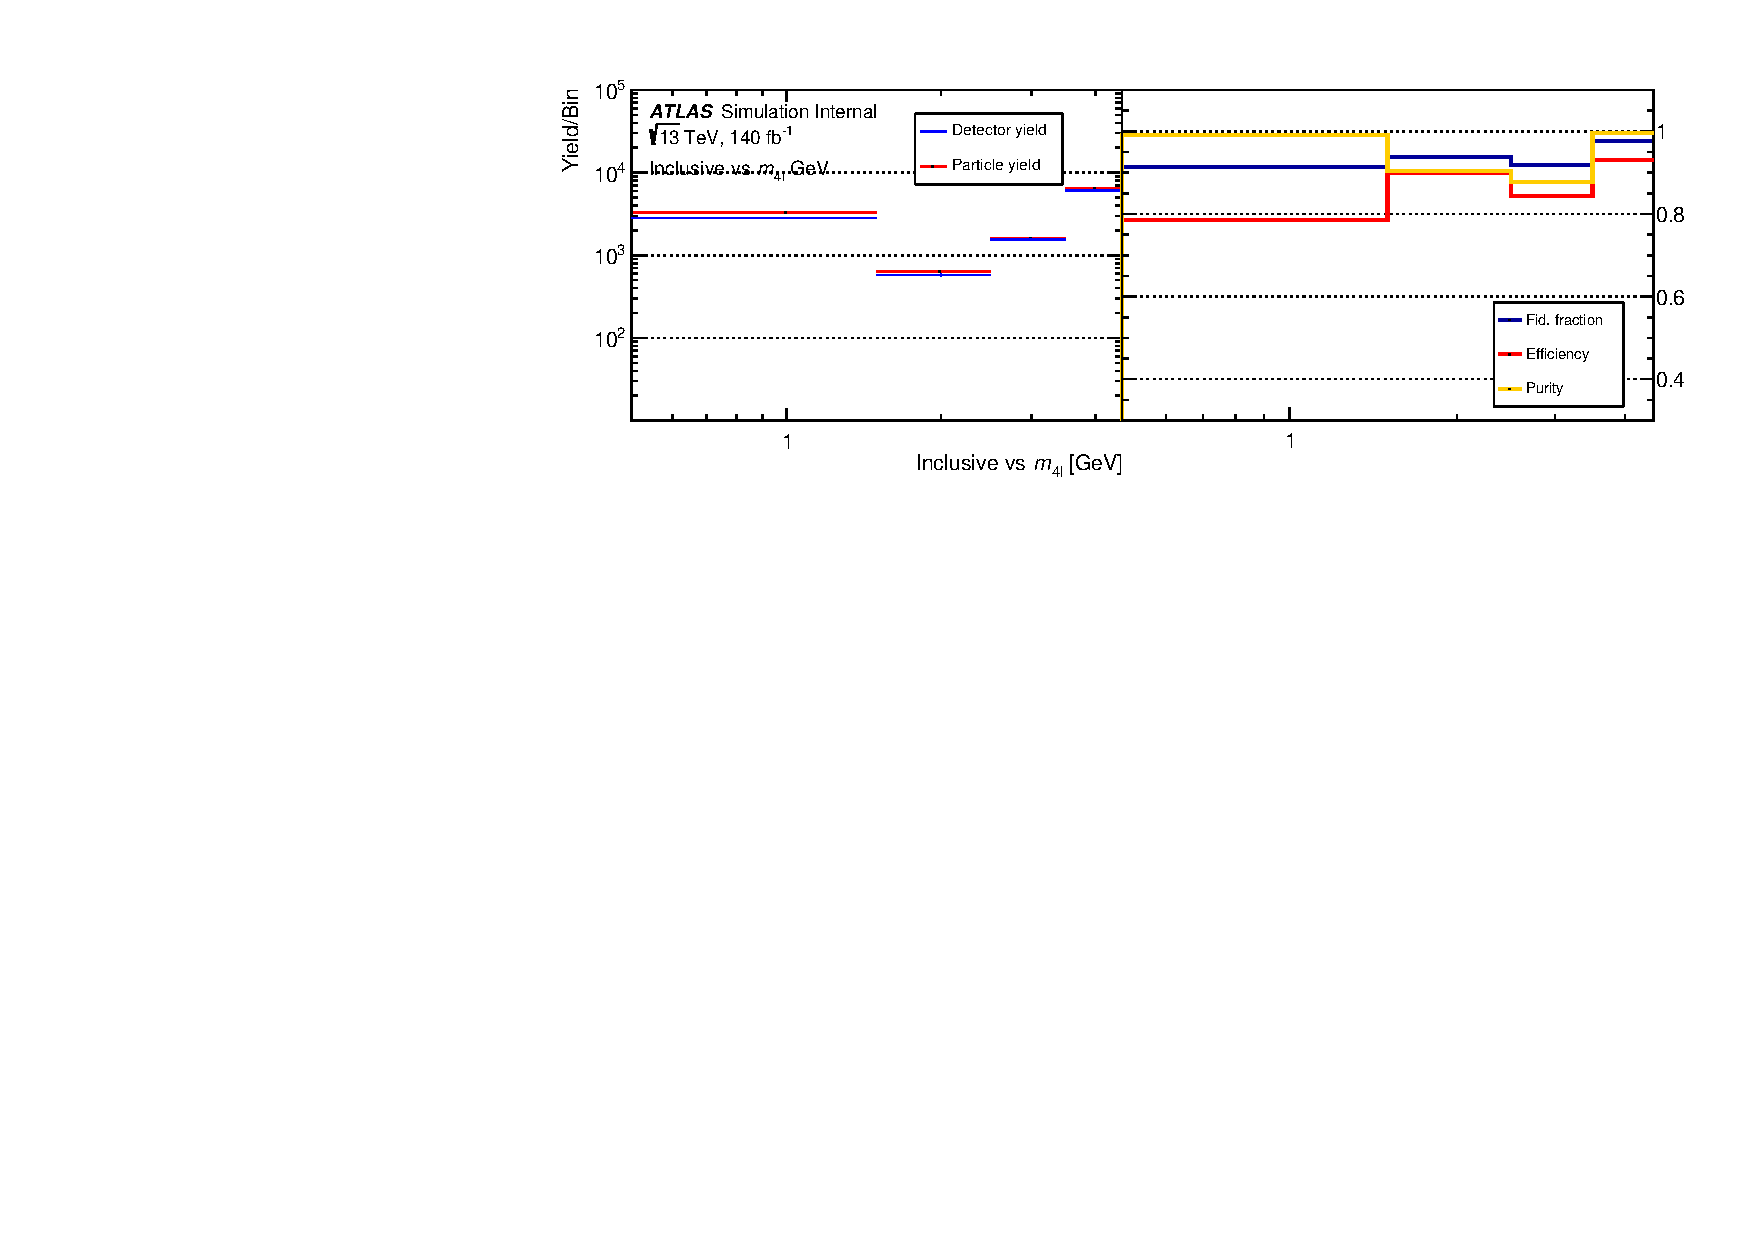
\includegraphics[width = 0.85\textwidth]{figures/UnfoldingStudies/v014_inputs/inclusive_vs_m4linputs.pdf}}
\caption{In the left-hand panel, the number of predicted events passing the reconstruction- and fiducial- level selections are displayed as the detector yield and particle yield, respectively. They are given as a function of the four \mFourL regions: single Z, Higgs,  offshell ZZ, and onshell ZZ in that order. The right-hand panel shows the efficiency, fiducial purity and fiducial fraction in each of the same \mFourL regions.}
  \label{fig:inclvm4lunf}
 \end{figure}  

%%inclusive vs m4l
\begin{figure}[htb]
  \centering 
  \subfigure{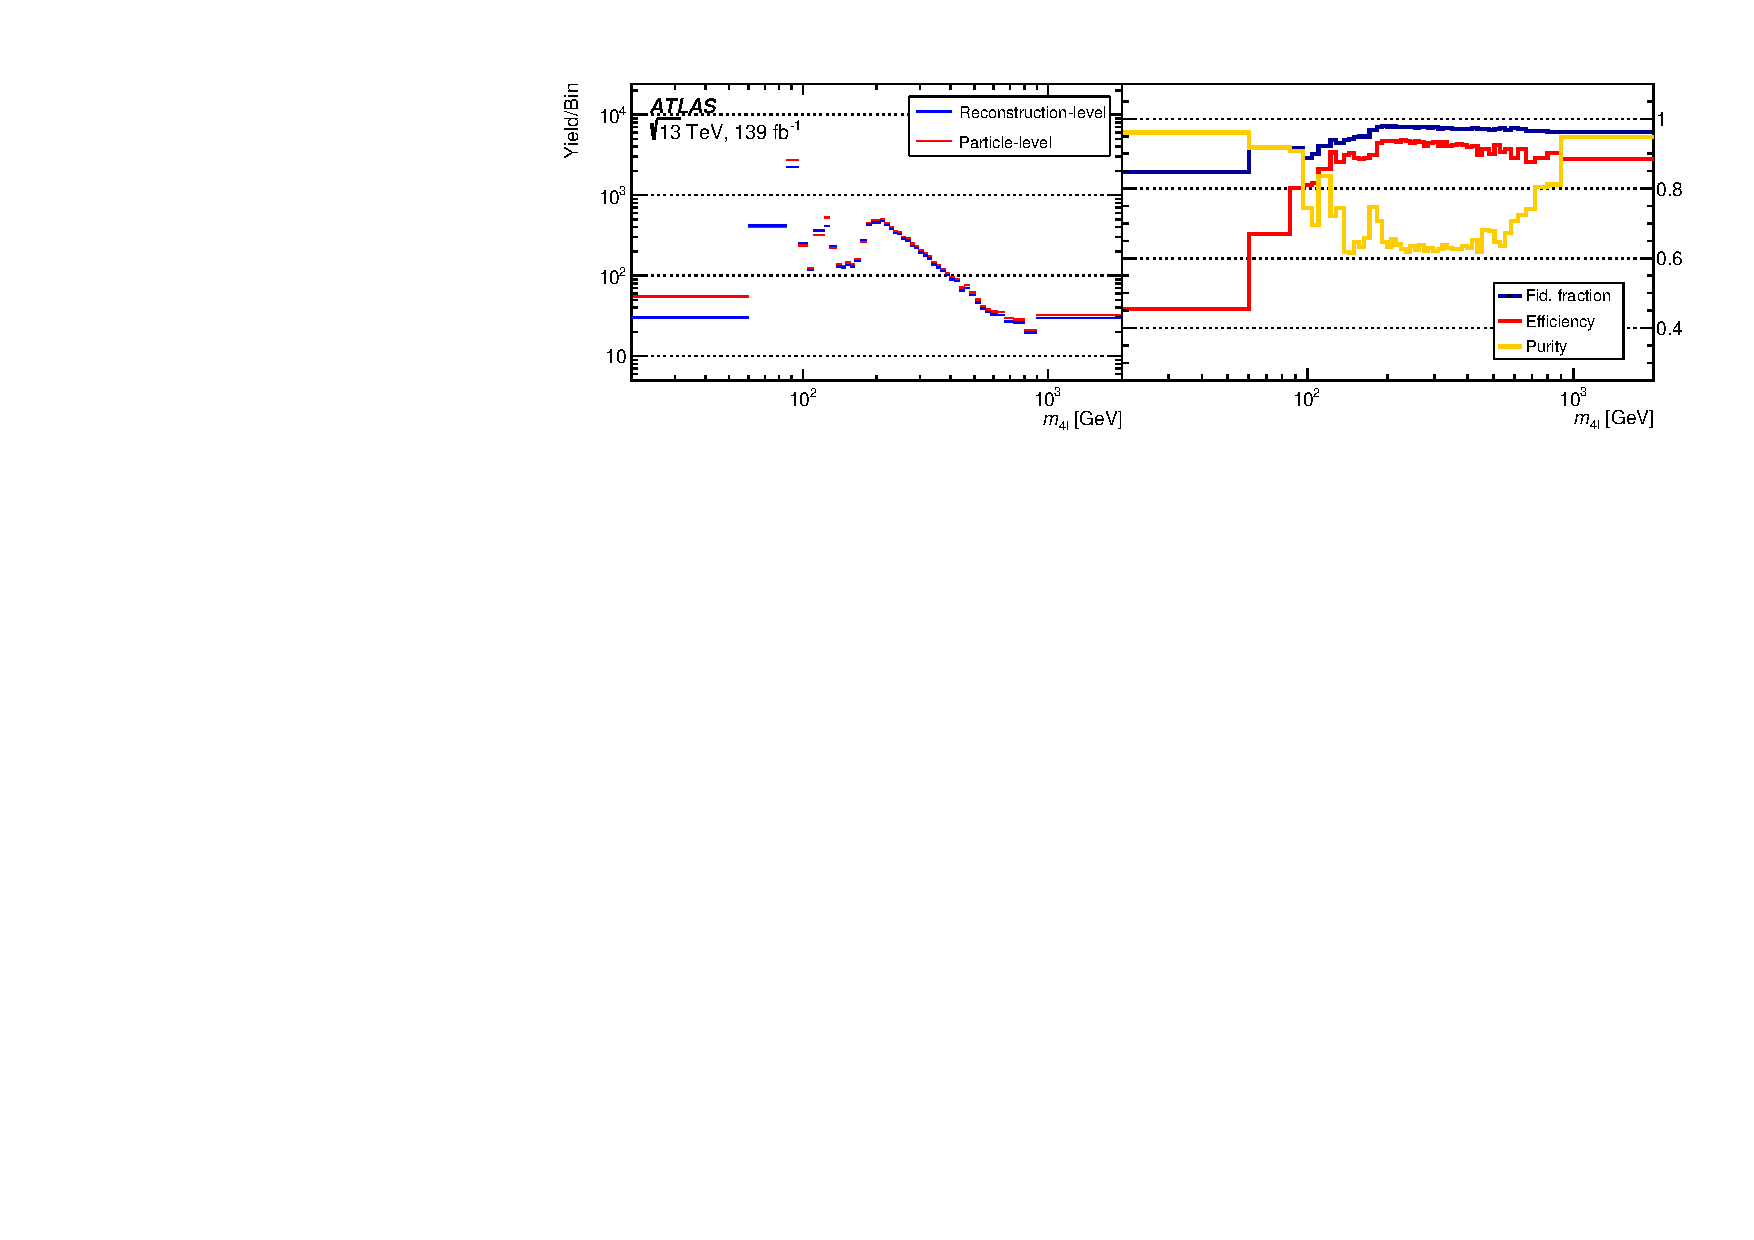
\includegraphics[width = 0.85\textwidth]{figures/UnfoldingStudies/v014_inputs/inclm4linputs.pdf}}
\caption{In the left-hand panel, the number of predicted events passing the reconstruction- and fiducial- level selections are displayed as the detector yield and particle yield, respectively. They are given as a function of inclusive \mFourL bins. The right-hand panel shows the efficiency, fiducial purity and fiducial fraction in each of the same \mFourL bins.}
 \end{figure} 

%%double differentials
\begin{figure}[htb]
  \centering 
  \subfigure{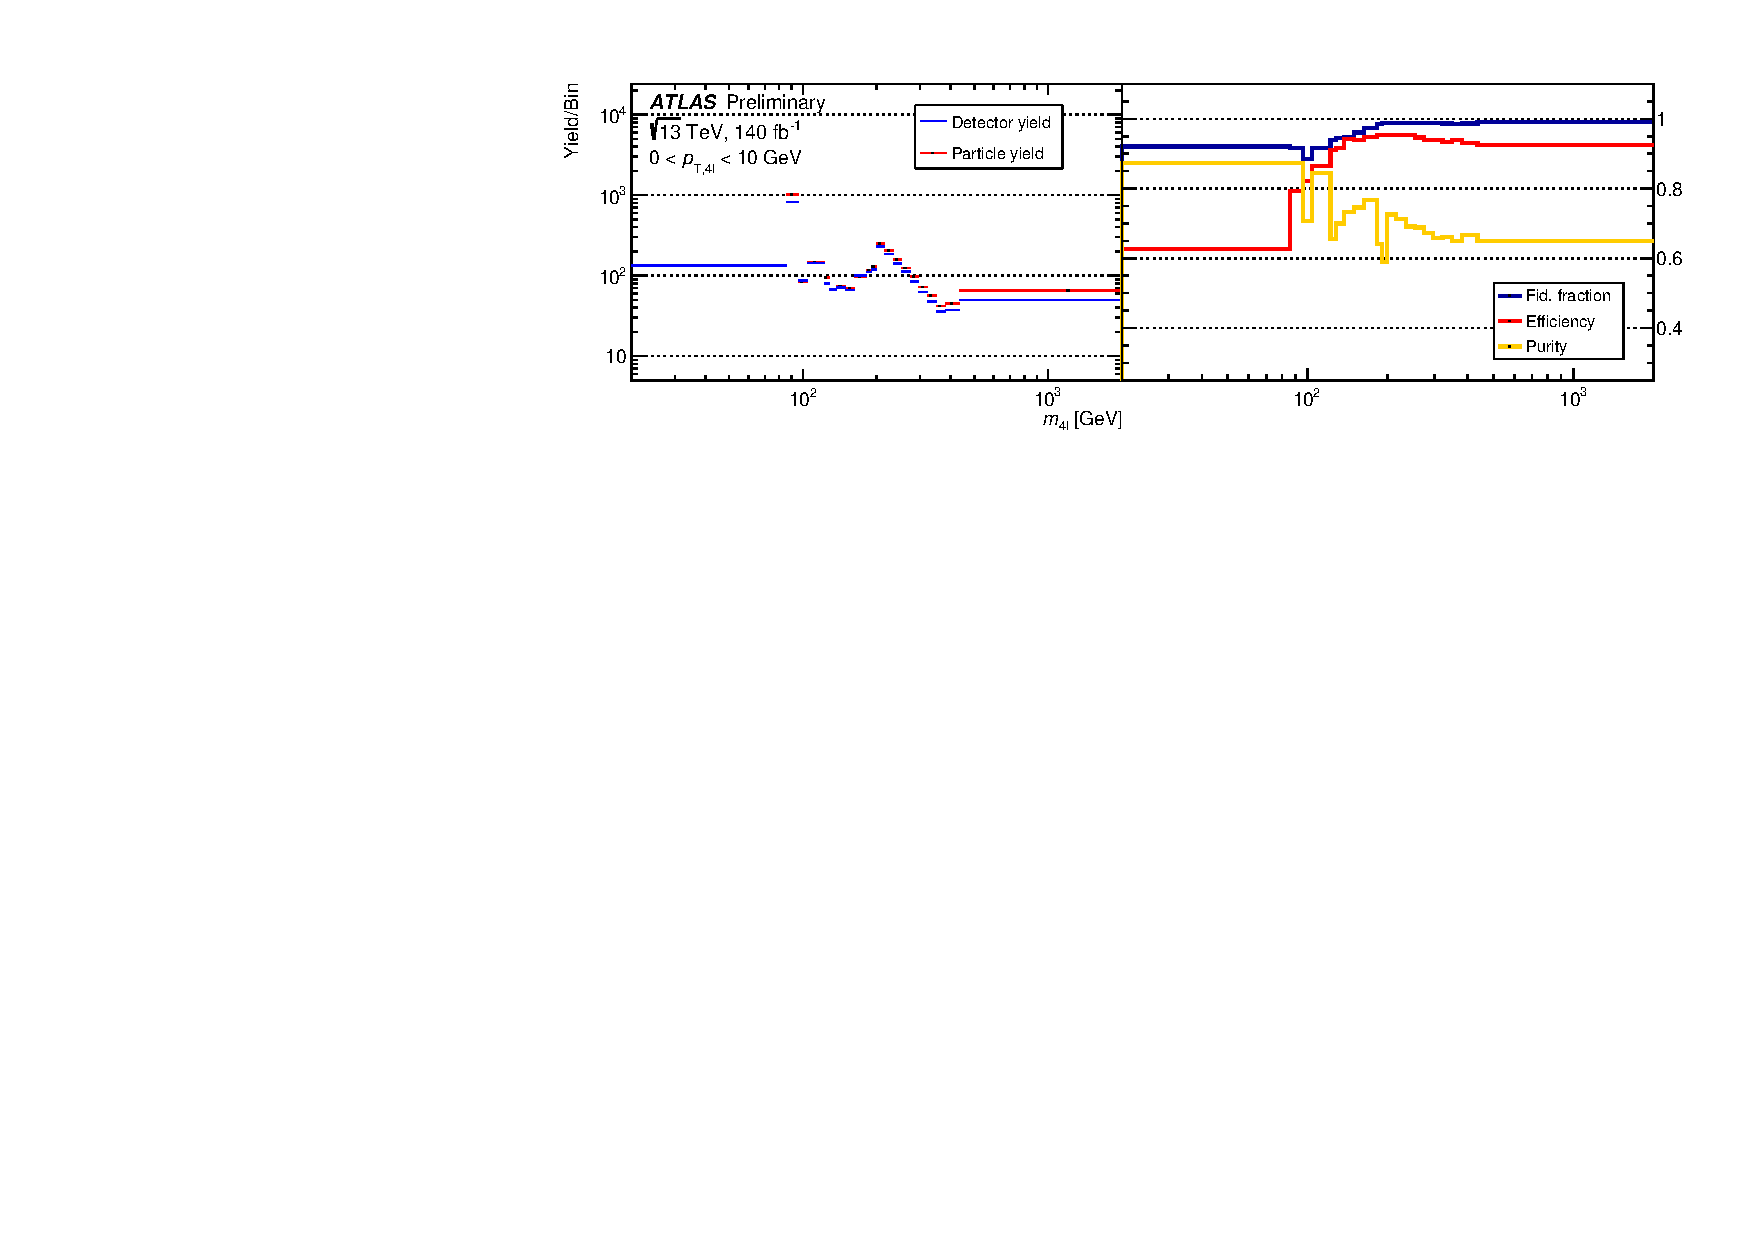
\includegraphics[width = 0.75\textwidth]{figures/UnfoldingStudies/v014_inputs/m4l_pt4l0-10inputs.pdf}}\\
\vspace{-1cm}
  \subfigure{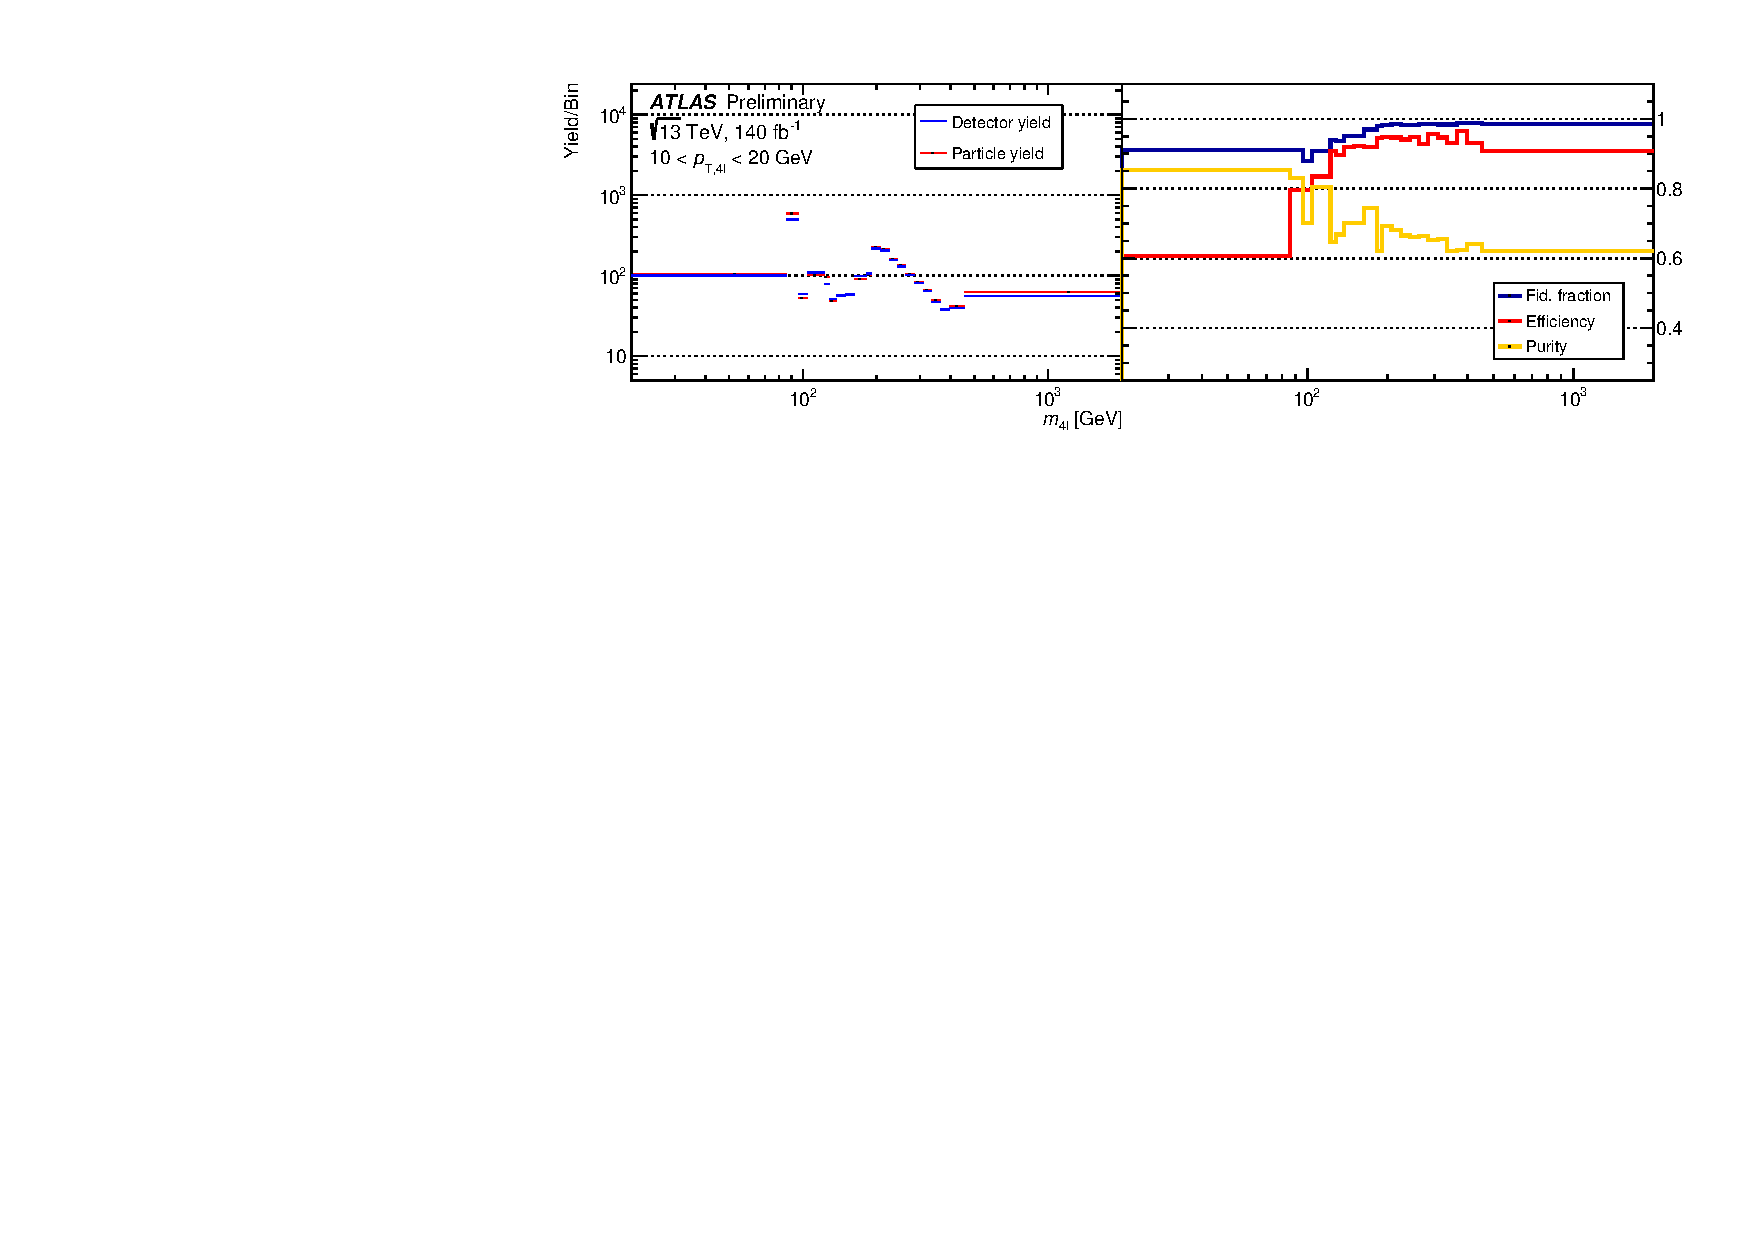
\includegraphics[width = 0.75\textwidth]{figures/UnfoldingStudies/v014_inputs/m4l_pt4l10-20inputs.pdf}}\\
\vspace{-1cm}
  \subfigure{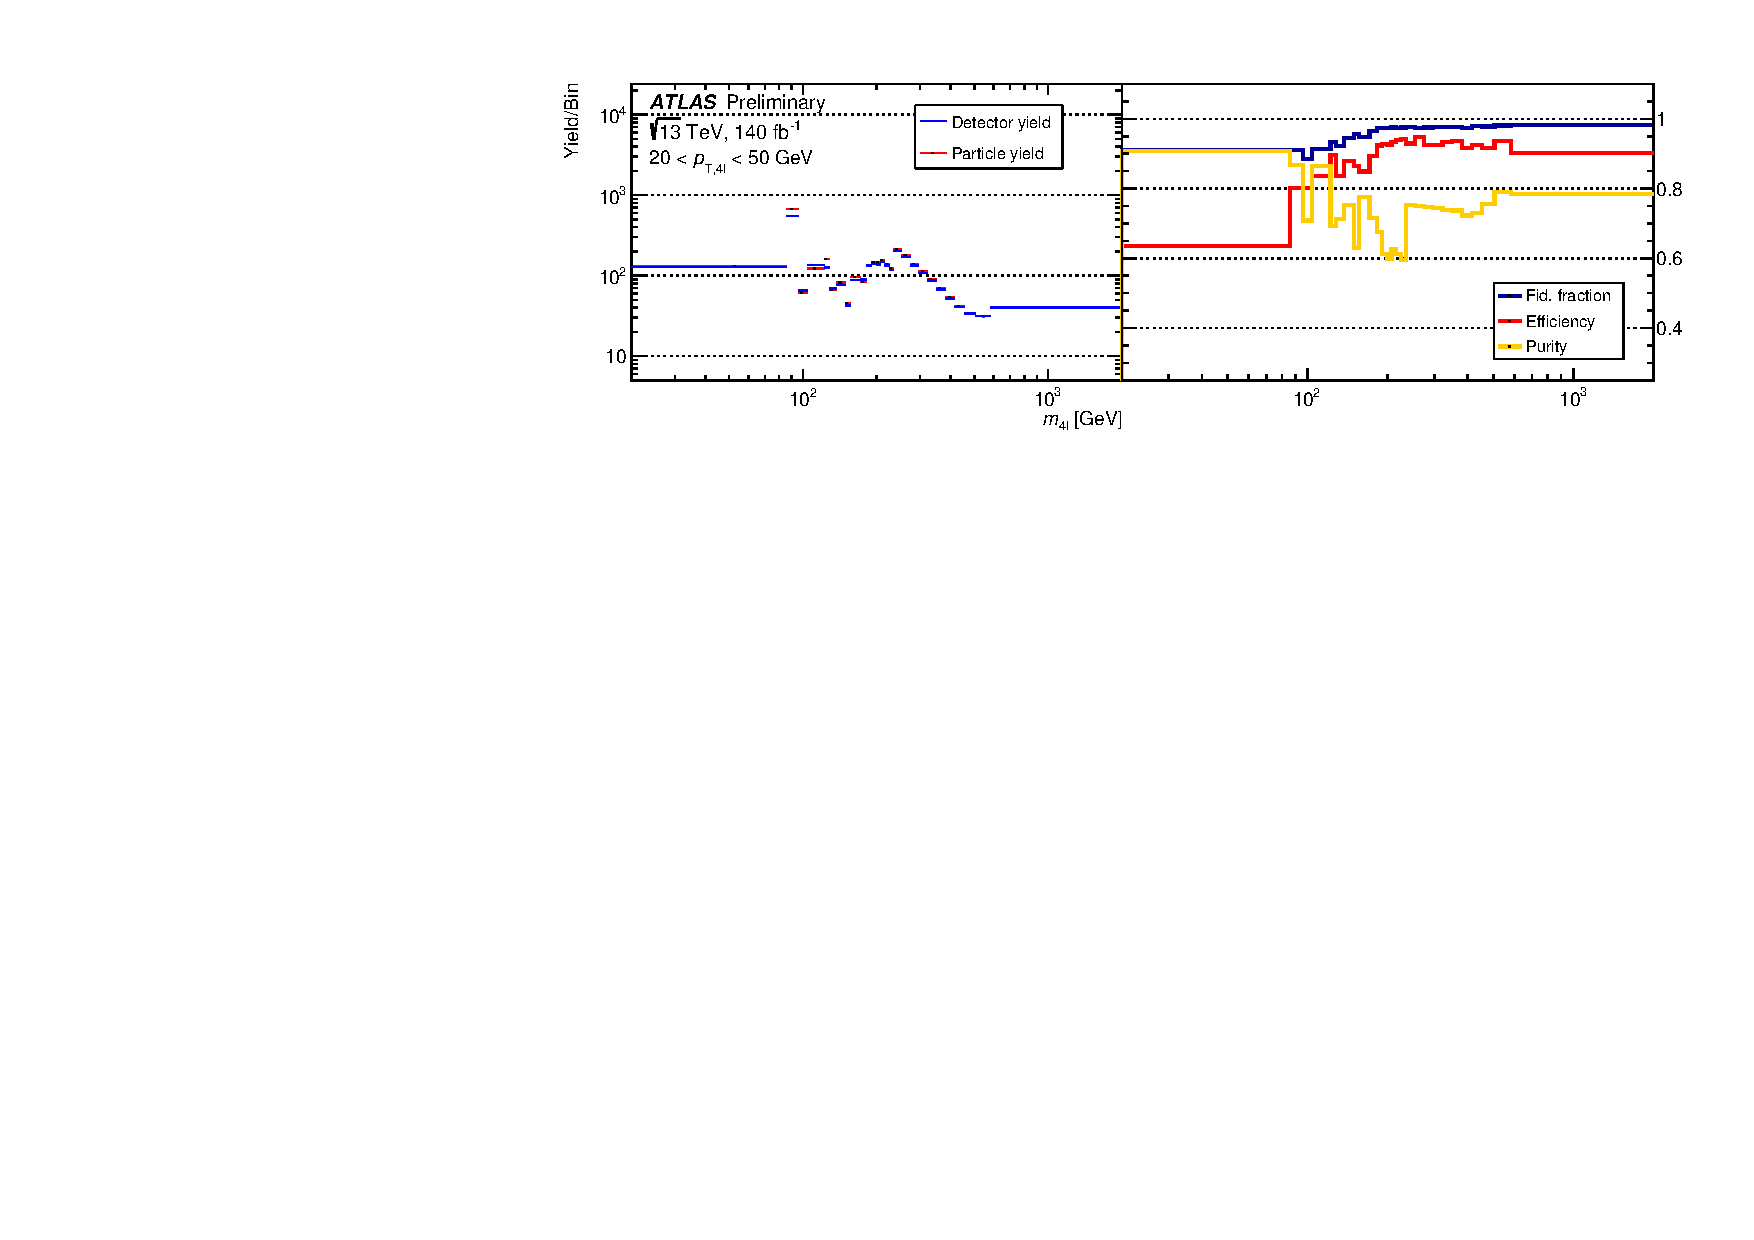
\includegraphics[width = 0.75\textwidth]{figures/UnfoldingStudies/v014_inputs/m4l_pt4l20-50inputs.pdf}}\\
\vspace{-1cm}
  \subfigure{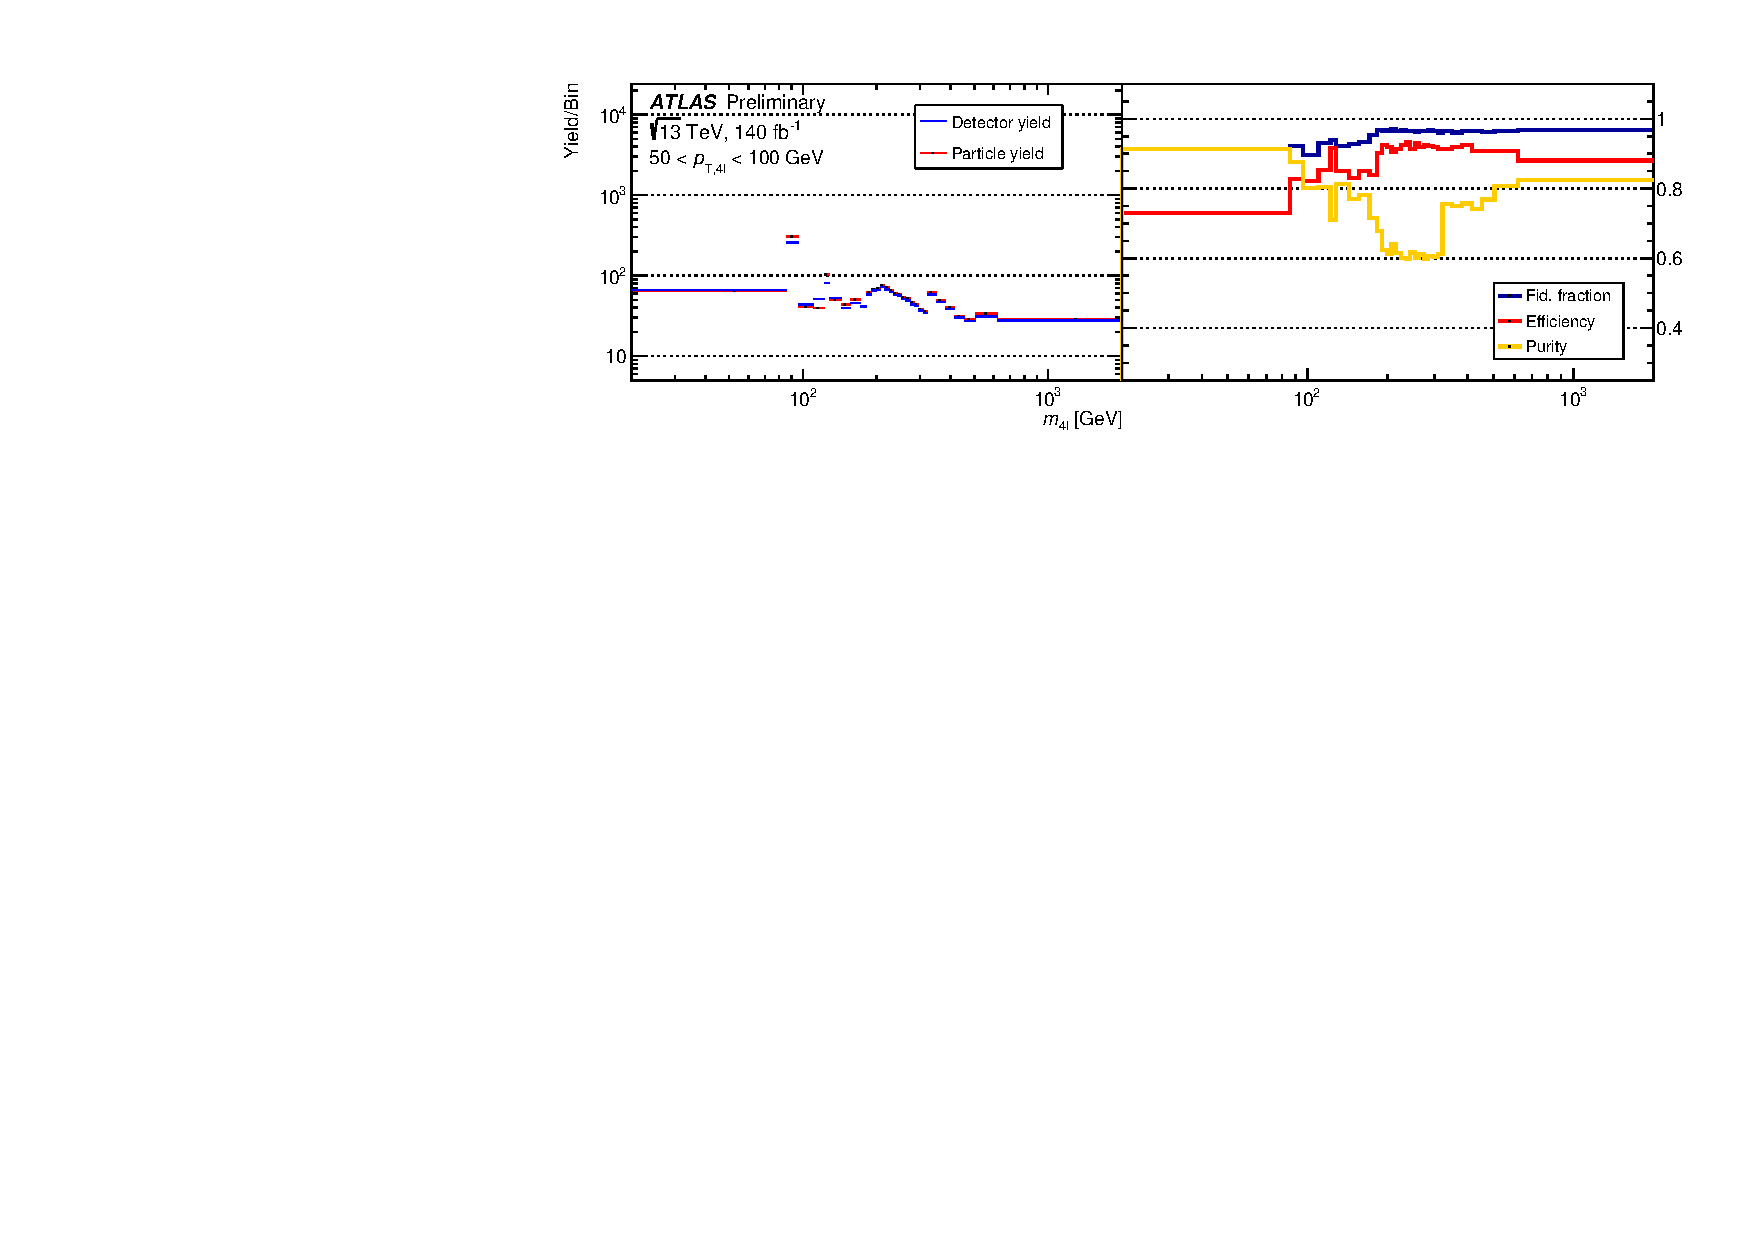
\includegraphics[width = 0.75\textwidth]{figures/UnfoldingStudies/v014_inputs/m4l_pt4l50-100inputs.pdf}}\\
\vspace{-1cm}
  \subfigure{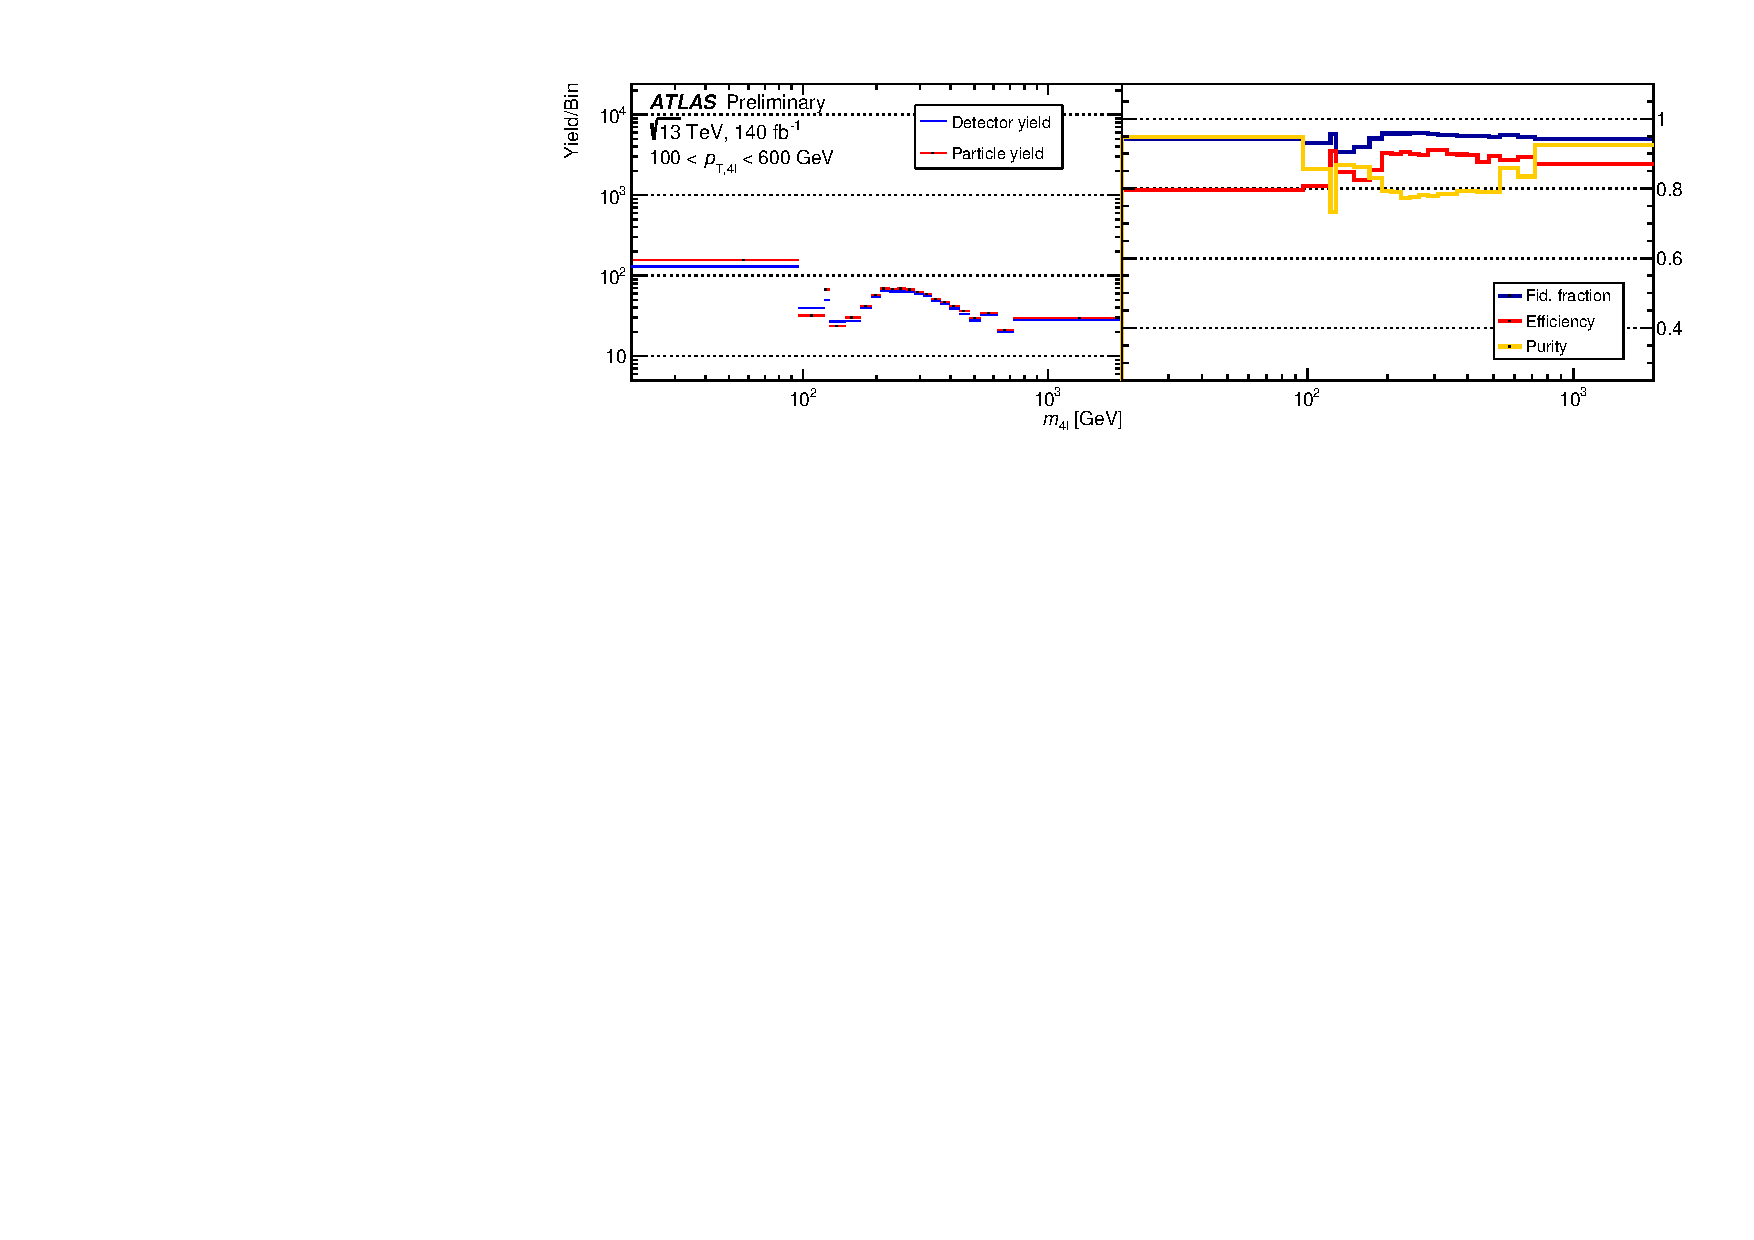
\includegraphics[width = 0.75\textwidth]{figures/UnfoldingStudies/v014_inputs/m4l_pt4l100-600inputs.pdf}}\\
\vspace{-0.5cm}
\caption{In the left-hand panels, the number of predicted events passing the reconstruction- and fiducial- level selections are displayed as the detector yield and particle yield, respectively. The right-hand panel shows the efficiency, fiducial purity and fiducial fraction. All variables are plotted as a function of the \mFourL bins, in slices of the \ptFourL variable which are stacked and labelled with the included \ptFourL range.
  \label{fig:pt4lunf}}
 \end{figure}  

\FloatBarrier
\clearpage

%y4l
\begin{figure}[htb]
  \centering 
  \subfigure{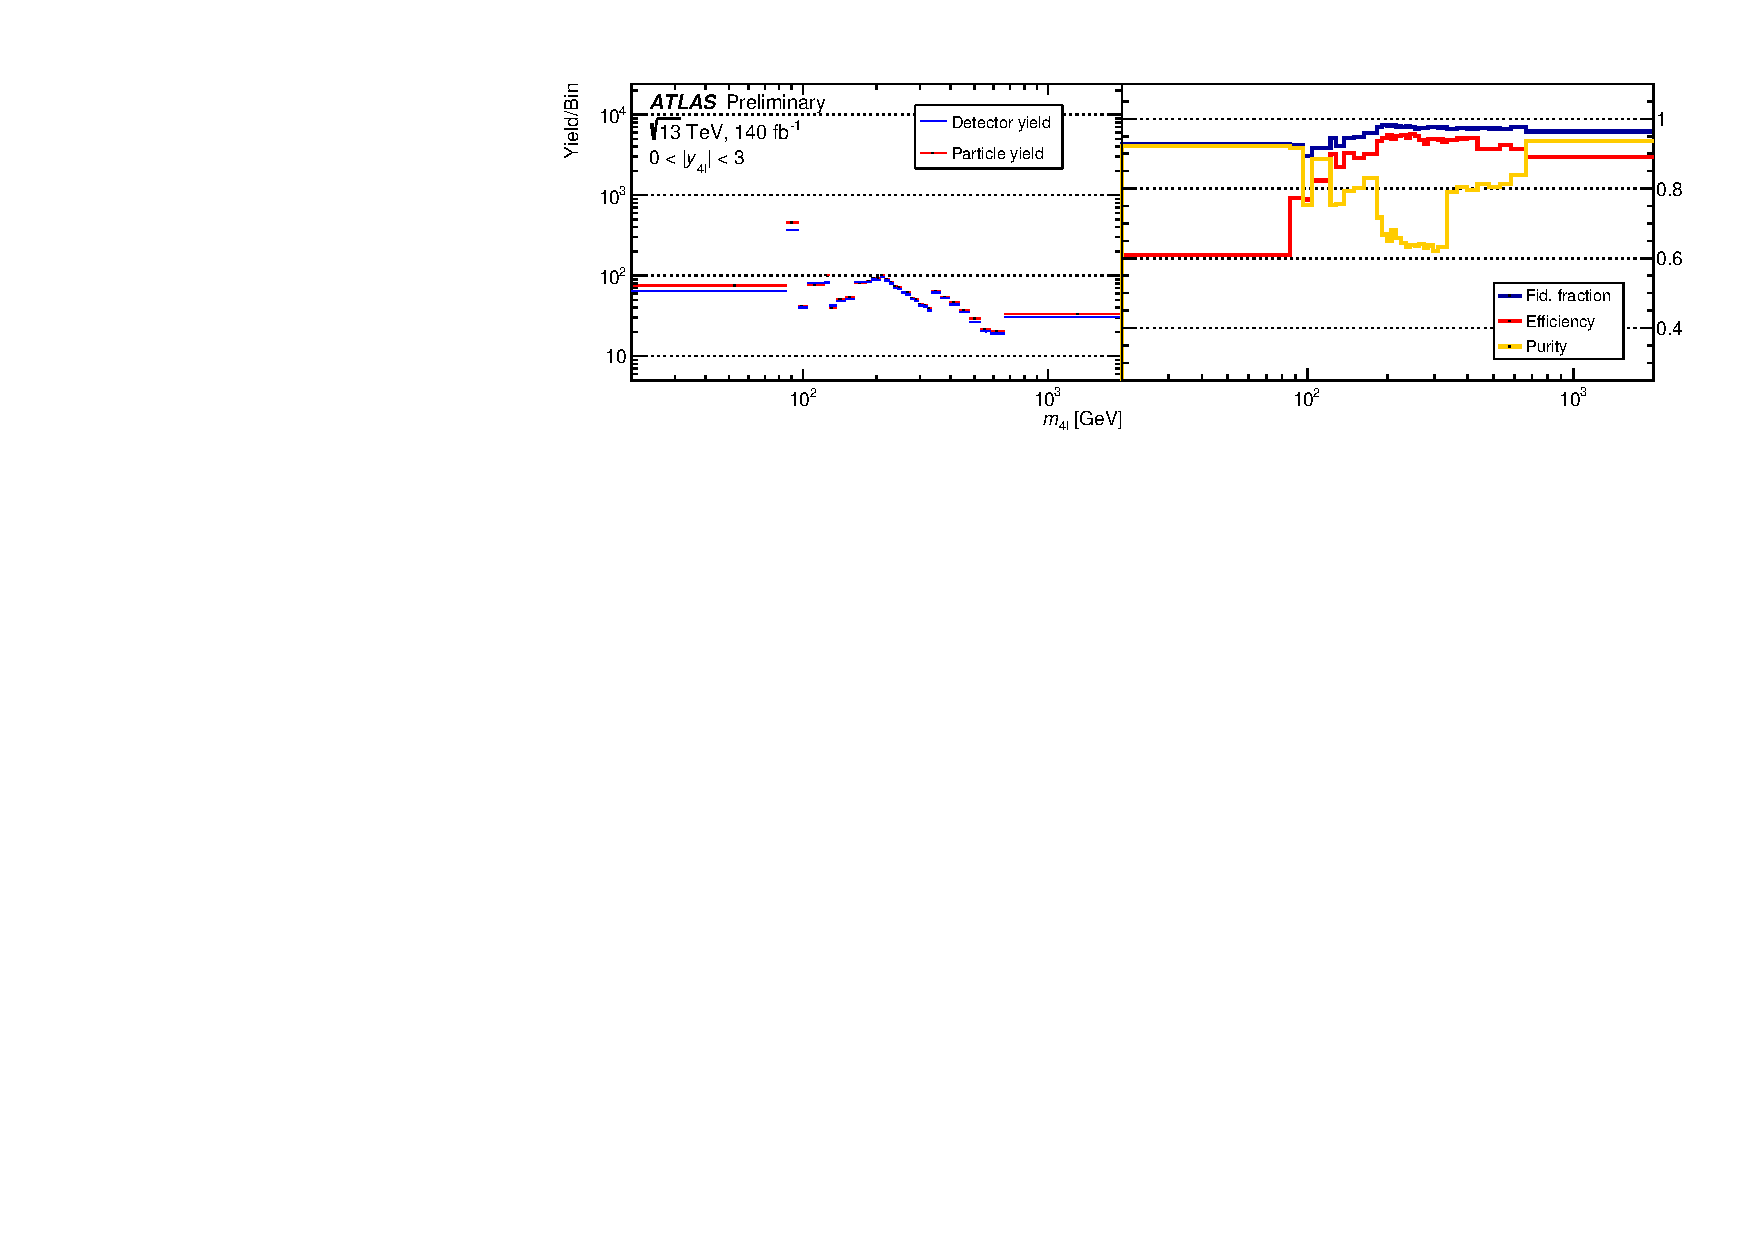
\includegraphics[width = 0.75\textwidth]{figures/UnfoldingStudies/v014_inputs/m4l_y4l0-3inputs.pdf}}\\
\vspace{-1cm}
  \subfigure{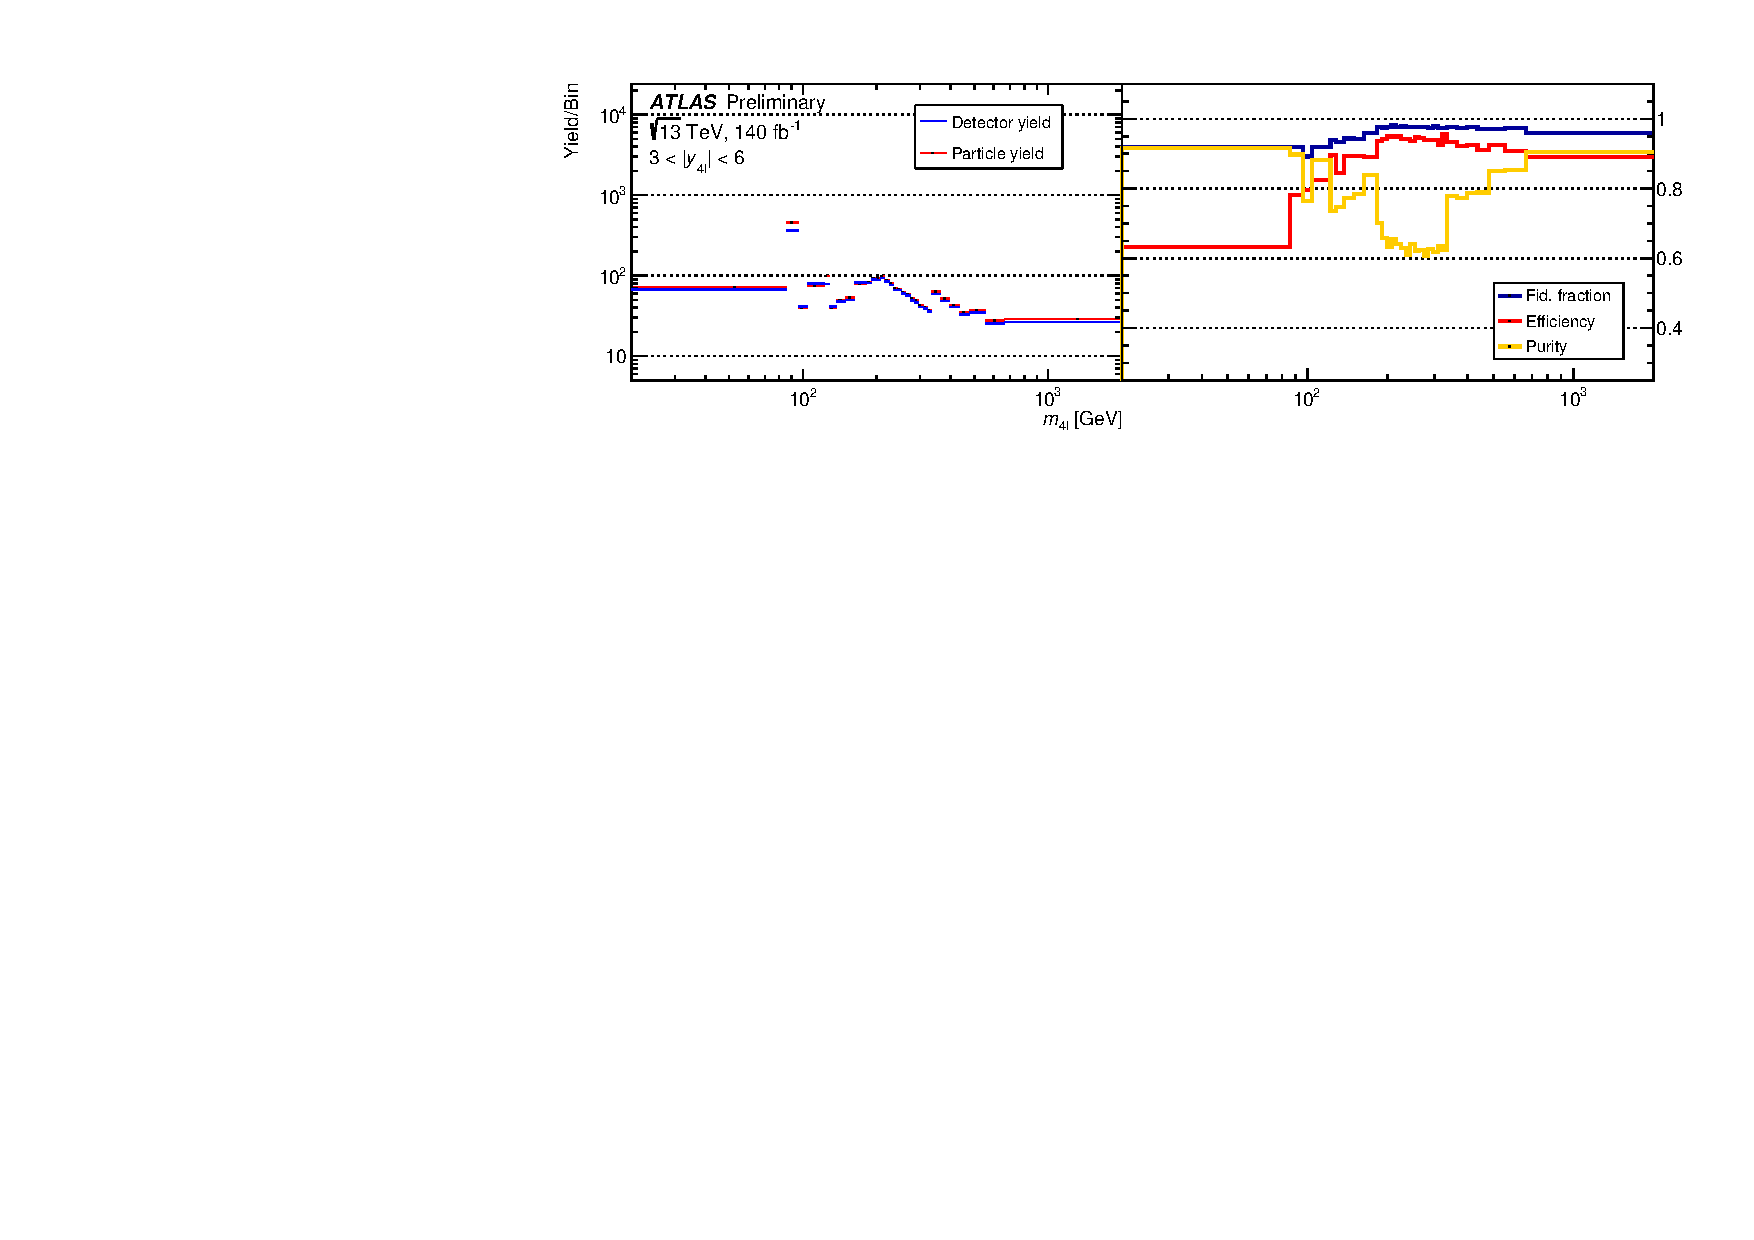
\includegraphics[width = 0.75\textwidth]{figures/UnfoldingStudies/v014_inputs/m4l_y4l3-6inputs.pdf}}\\
\vspace{-1cm}
  \subfigure{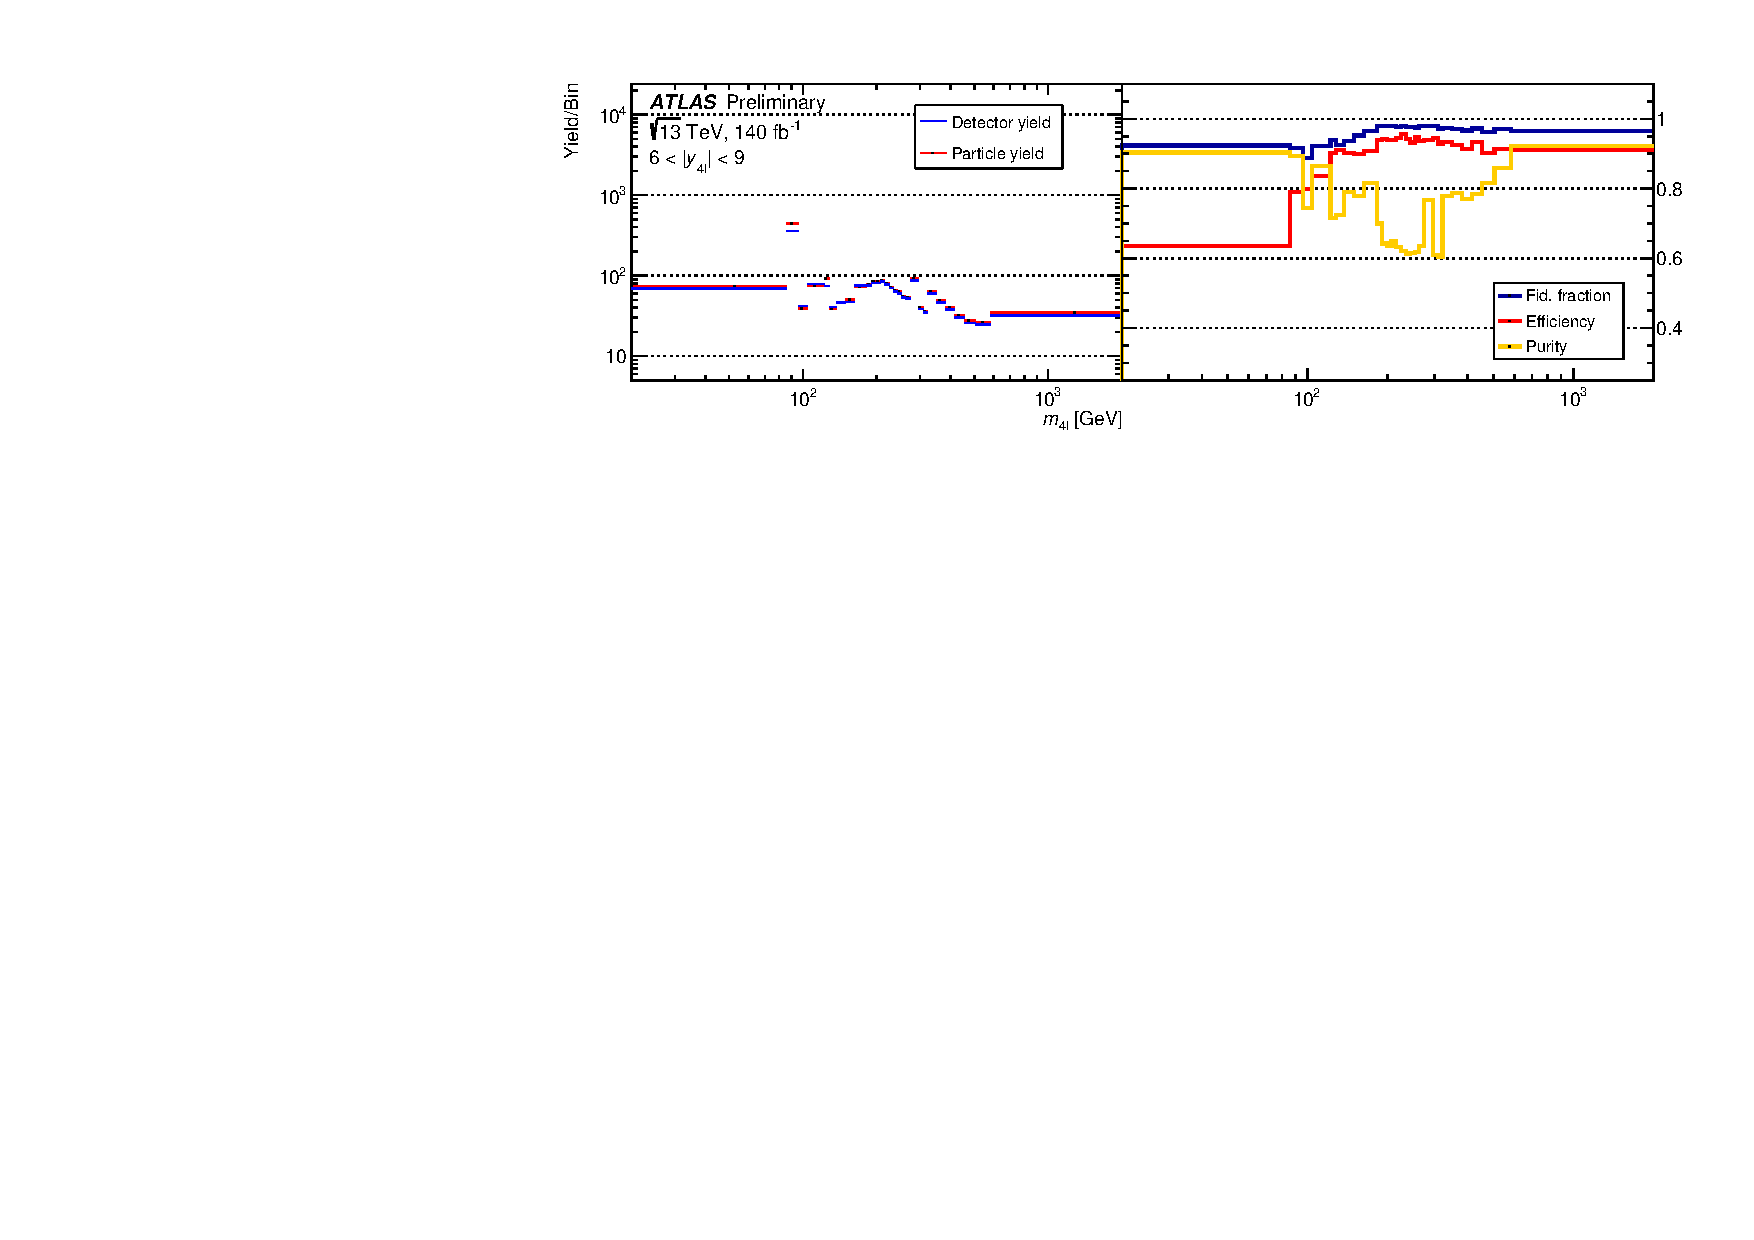
\includegraphics[width = 0.75\textwidth]{figures/UnfoldingStudies/v014_inputs/m4l_y4l6-9inputs.pdf}}\\
\vspace{-1cm}
  \subfigure{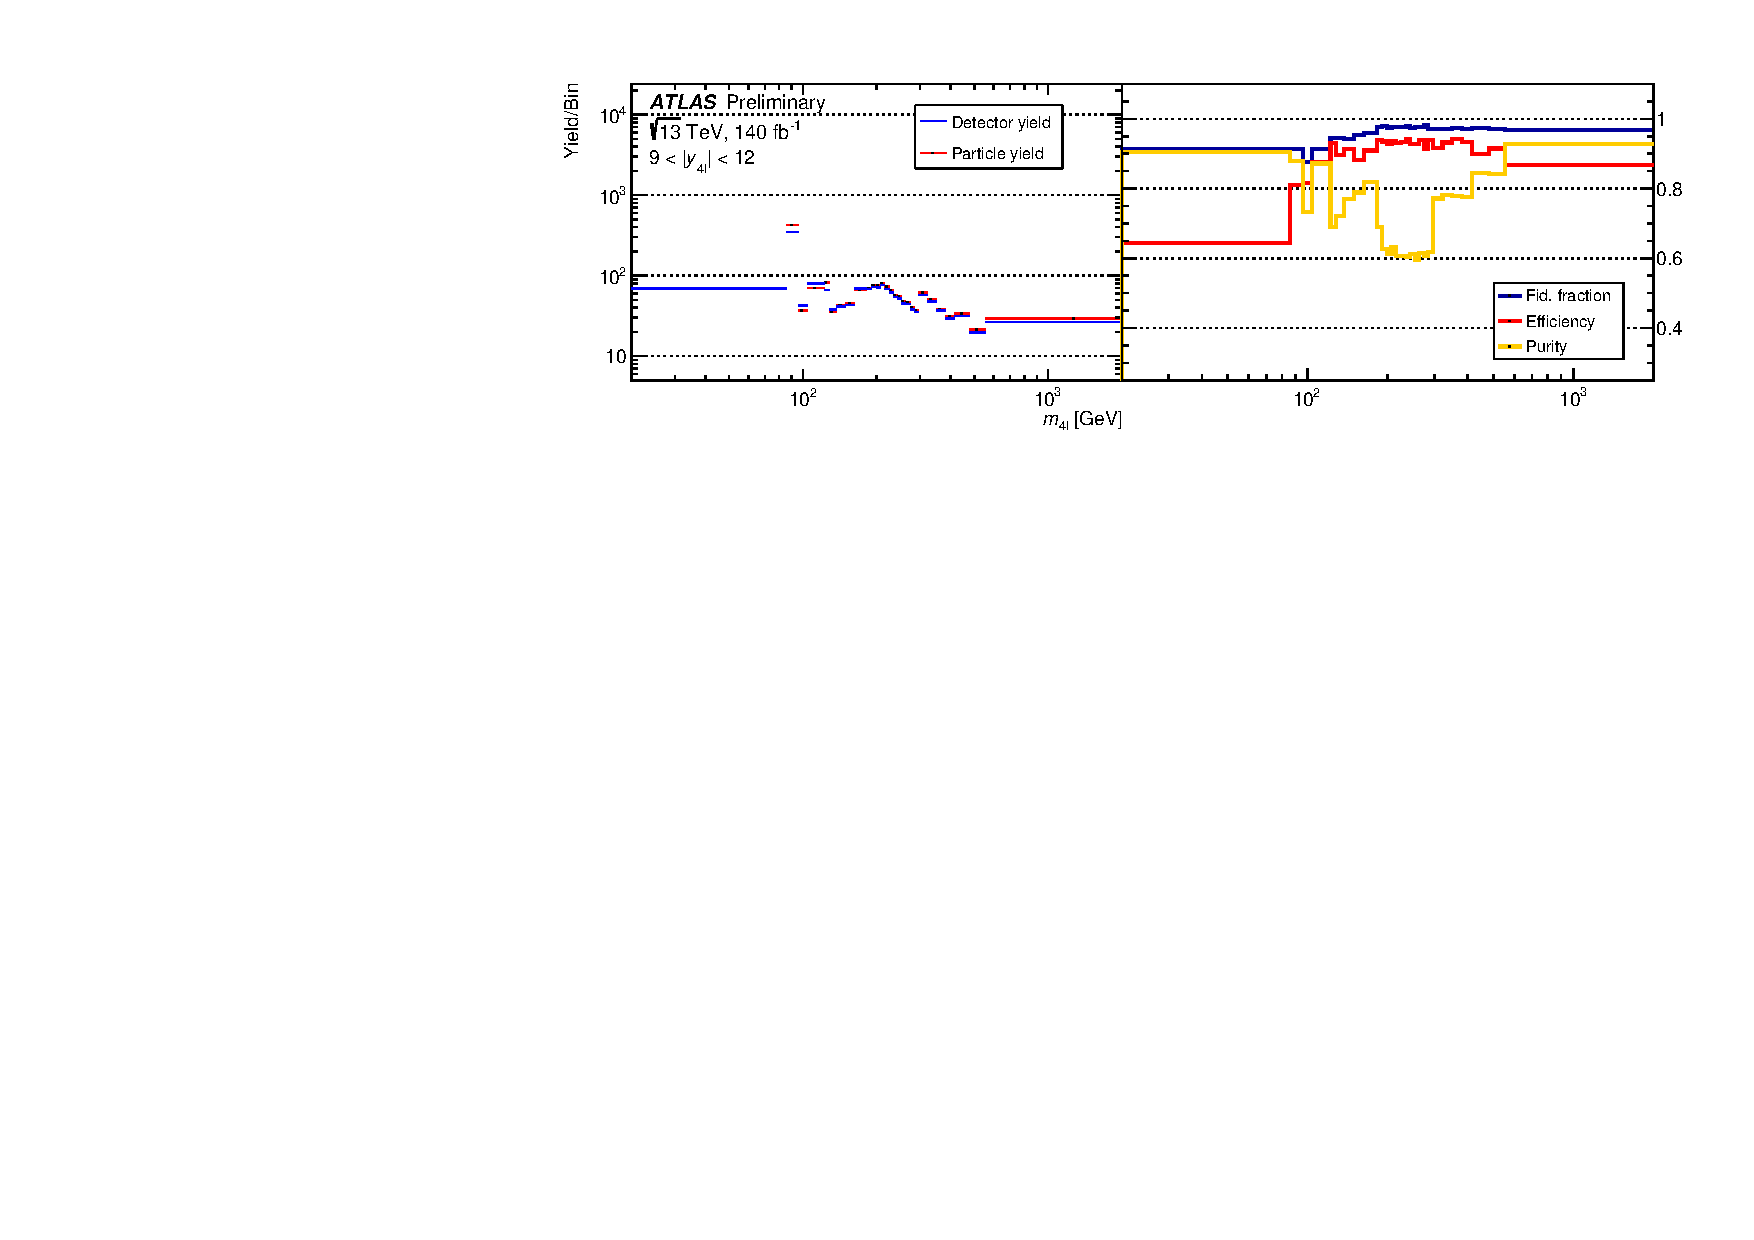
\includegraphics[width = 0.75\textwidth]{figures/UnfoldingStudies/v014_inputs/m4l_y4l9-12inputs.pdf}}\\
\vspace{-1cm}
  \subfigure{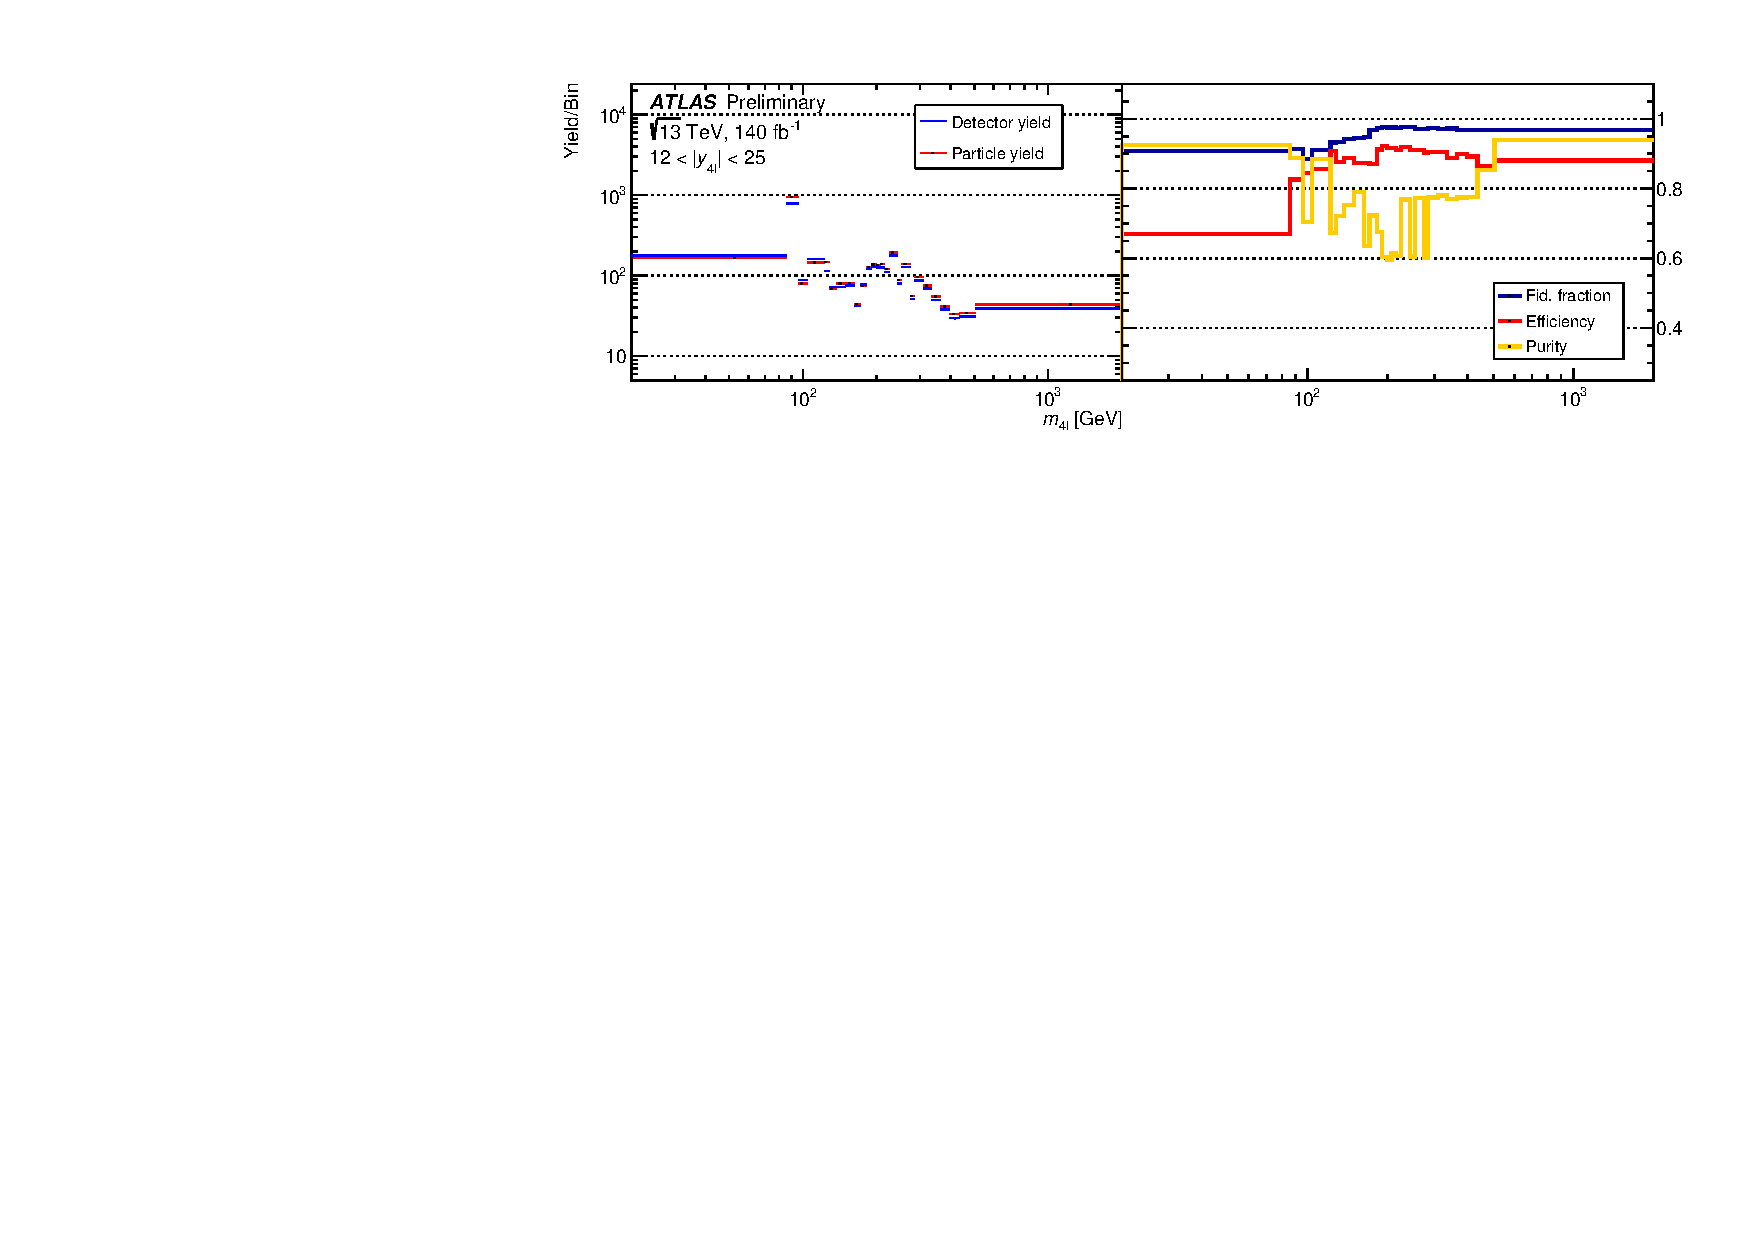
\includegraphics[width = 0.75\textwidth]{figures/UnfoldingStudies/v014_inputs/m4l_y4l12-25inputs.pdf}}\\
\vspace{-0.5cm}
\caption{In the left-hand panels, the number of predicted events passing the reconstruction- and fiducial- level selections are displayed as the detector yield and particle yield, respectively. The right-hand panel shows the efficiency, fiducial purity and fiducial fraction. All variables are plotted as a function of the \mFourL bins, in slices of the \yFourL variable which are stacked and labelled with the included \yFourL range.
  \label{fig:y4lunf}}
 \end{figure}  

\FloatBarrier
\clearpage

\begin{figure}[htb]
  \centering 
%elecs
  \subfigure{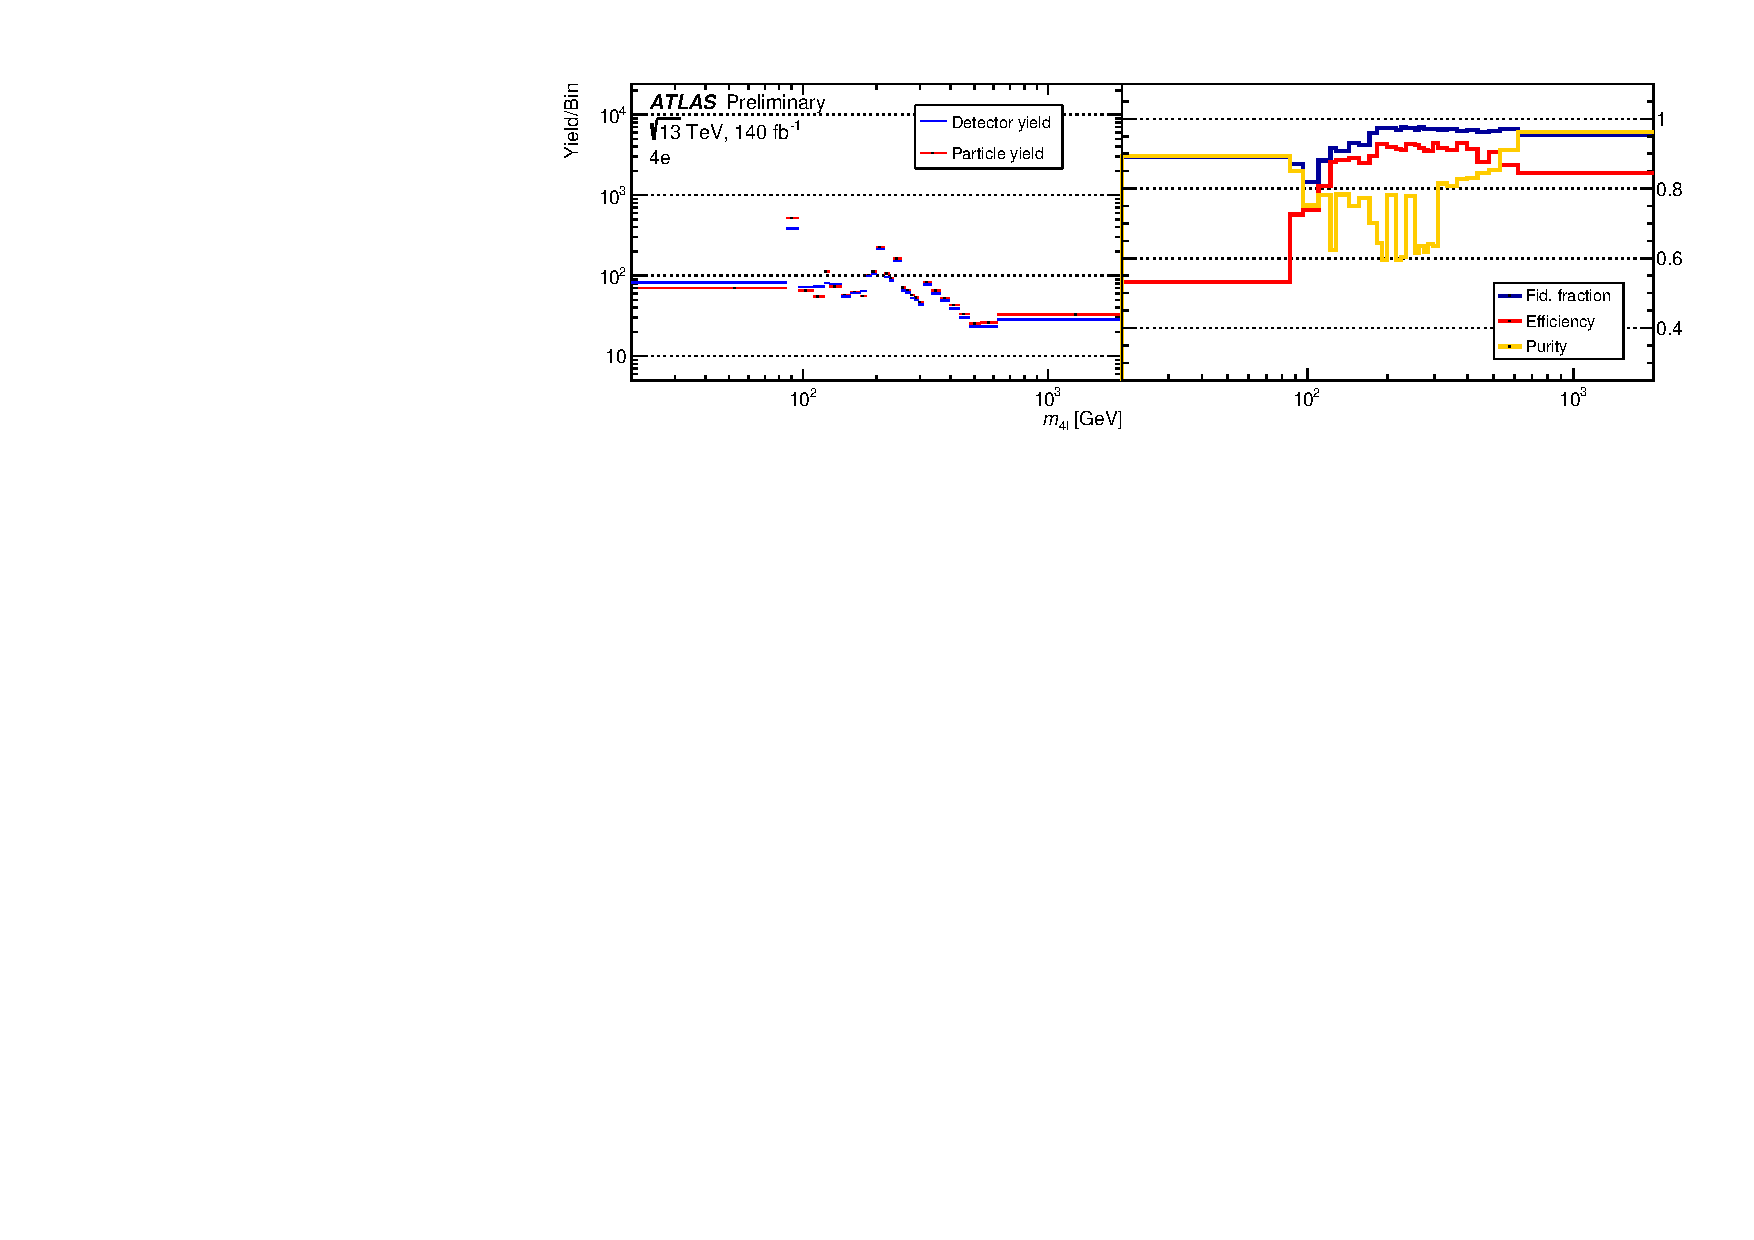
\includegraphics[width = 0.75\textwidth]{figures/UnfoldingStudies/v014_inputs/m4l_event_type0-1inputs.pdf}}\\
%muons
  \subfigure{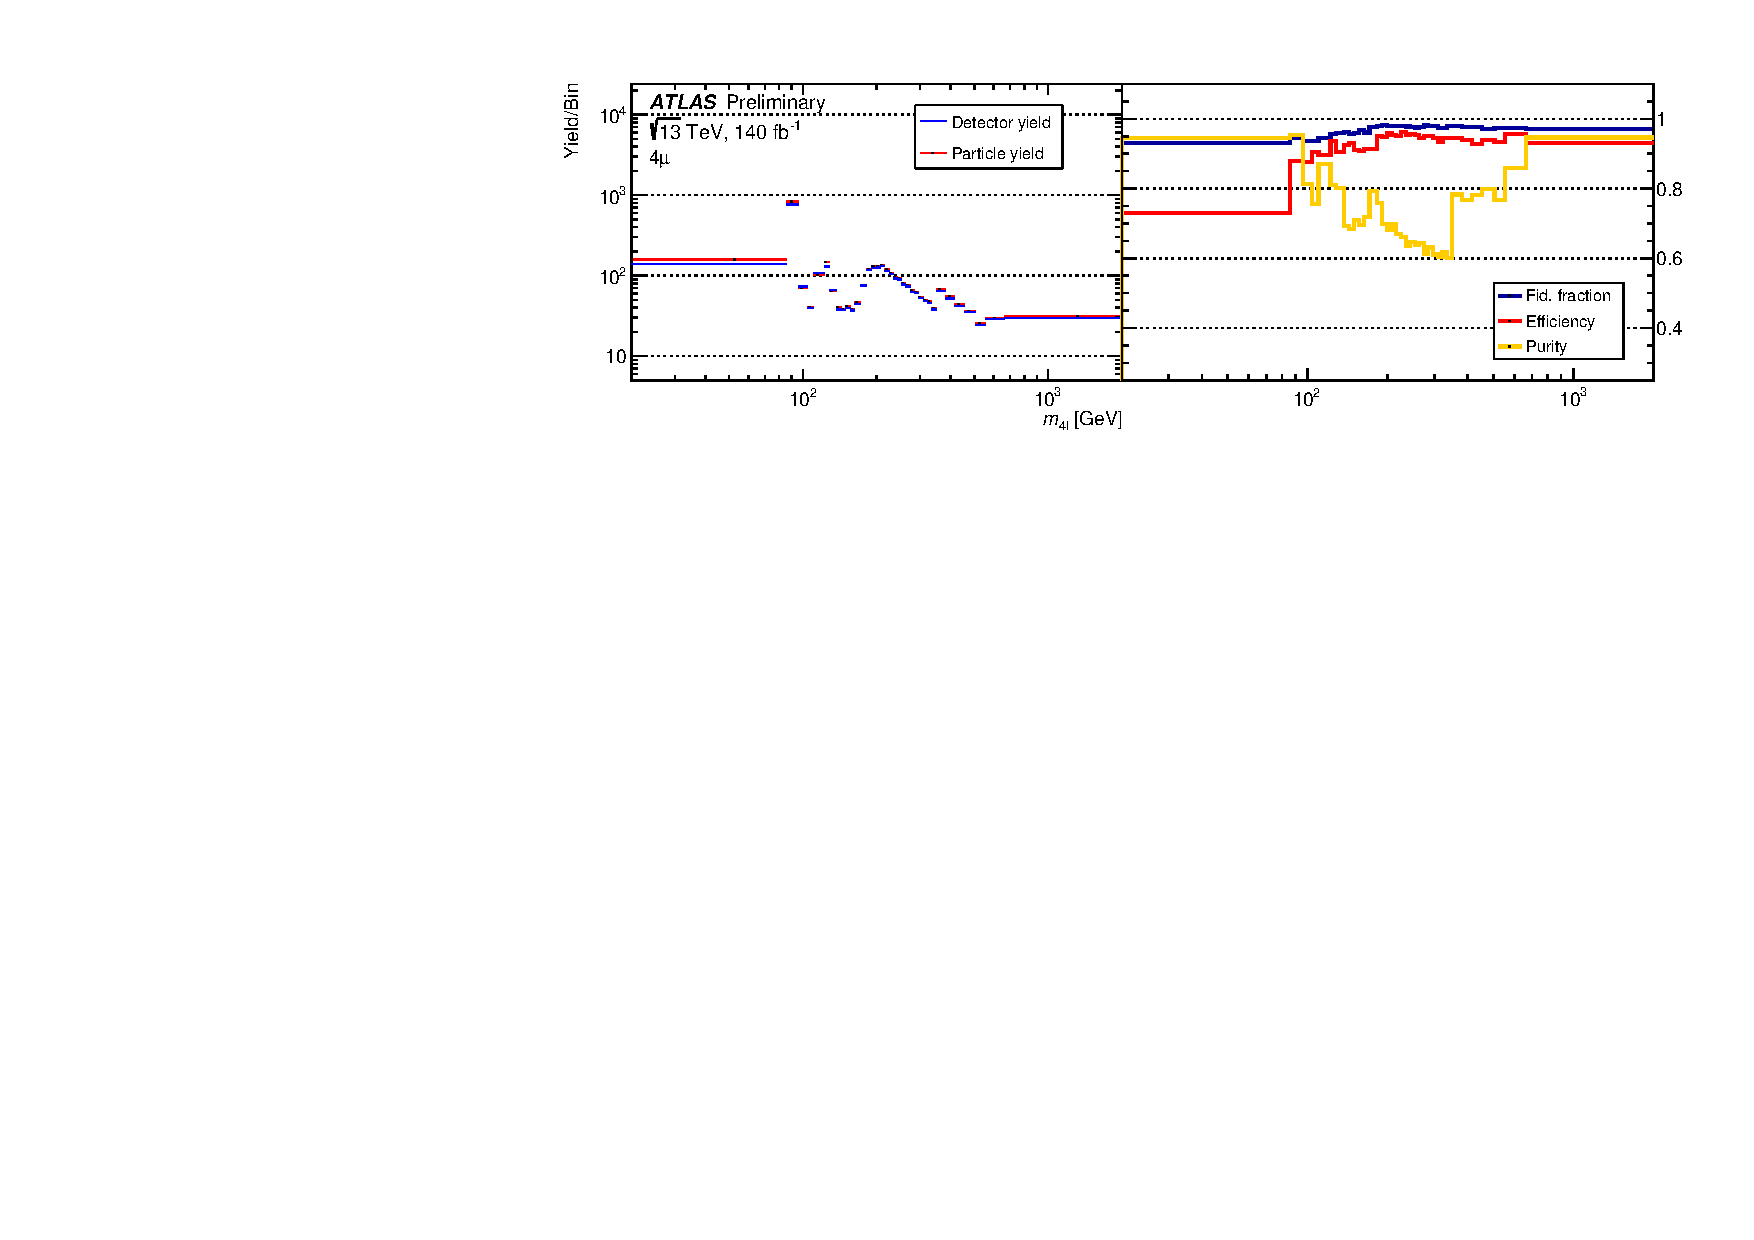
\includegraphics[width = 0.75\textwidth]{figures/UnfoldingStudies/v014_inputs/m4l_event_type0-0inputs.pdf}}\\
%2mu2e
  \subfigure{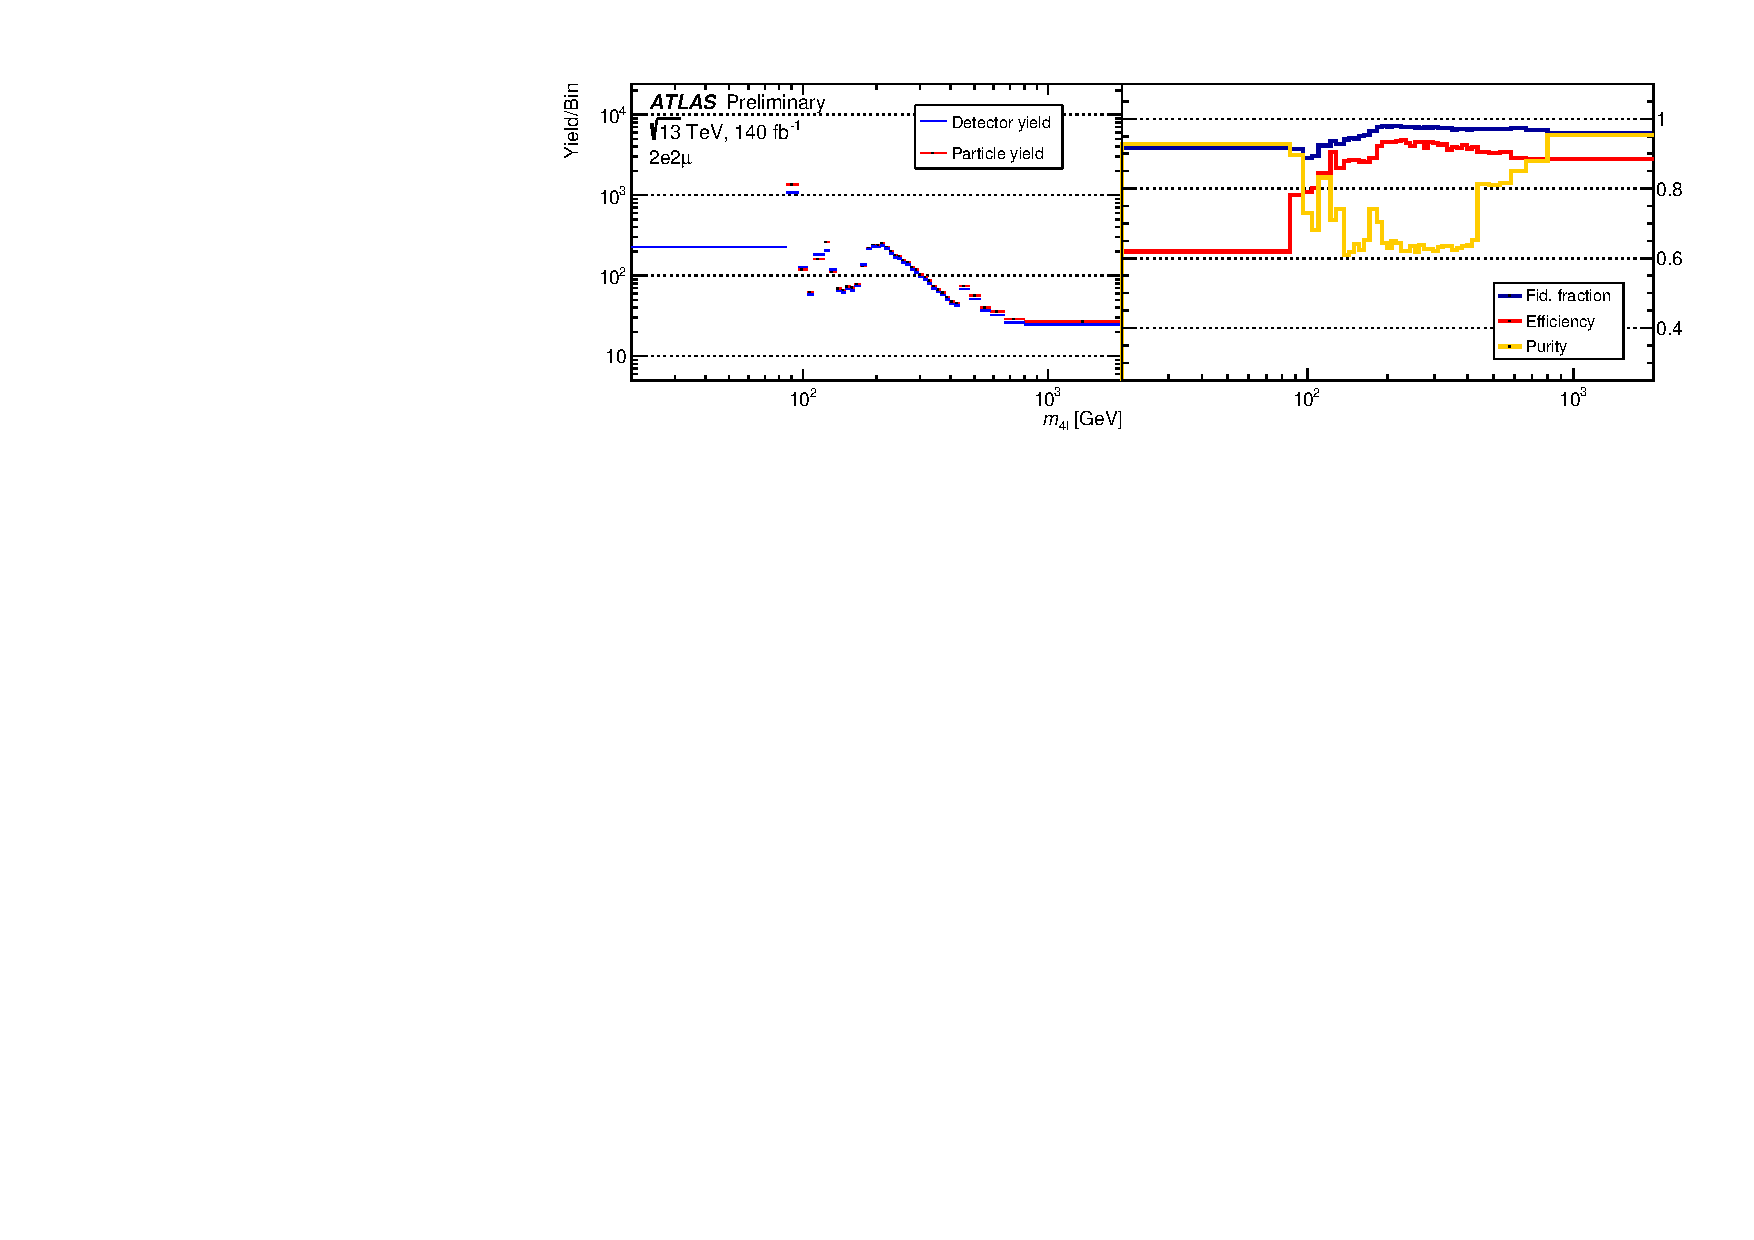
\includegraphics[width = 0.75\textwidth]{figures/UnfoldingStudies/v014_inputs/m4l_event_type1-3inputs.pdf}}\\
\caption{In the left-hand panels, the number of predicted events passing the reconstruction- and fiducial- level selections are displayed as the detector yield and particle yield, respectively. The right-hand panel shows the efficiency, fiducial purity and fiducial fraction. All variables are plotted as a function of the \mFourL bins, in the $4e$, $4\mu$ and $2e2\mu$ flavour channels from top to bottom.
  \label{fig:chunf}}
 \end{figure}  

\FloatBarrier
\clearpage

%%double differentials in coarse mass bins
%Z variables
\begin{figure}[htb]
  \centering 
  \subfigure{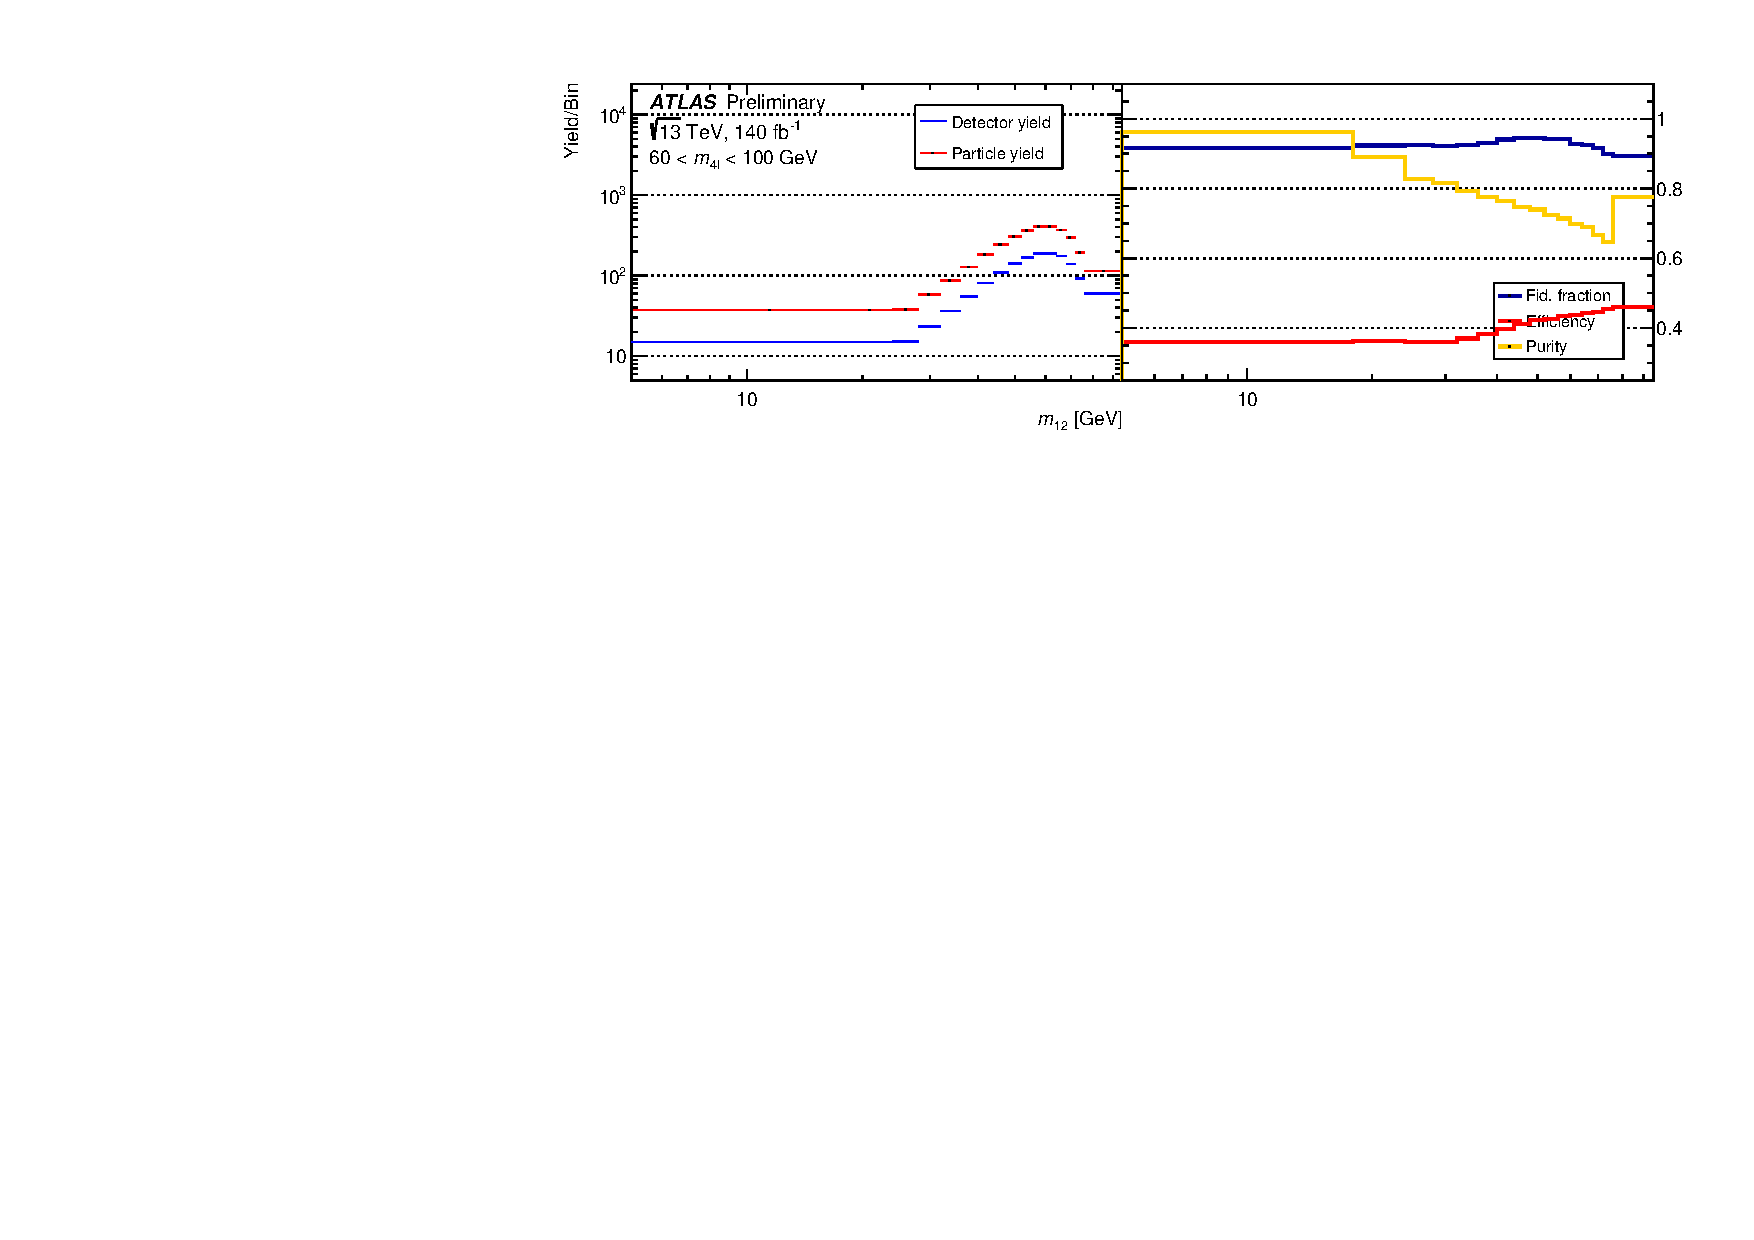
\includegraphics[width = 0.75\textwidth]{figures/UnfoldingStudies/v014_inputs/m12_m4l60-100inputs.pdf}}\\
  \subfigure{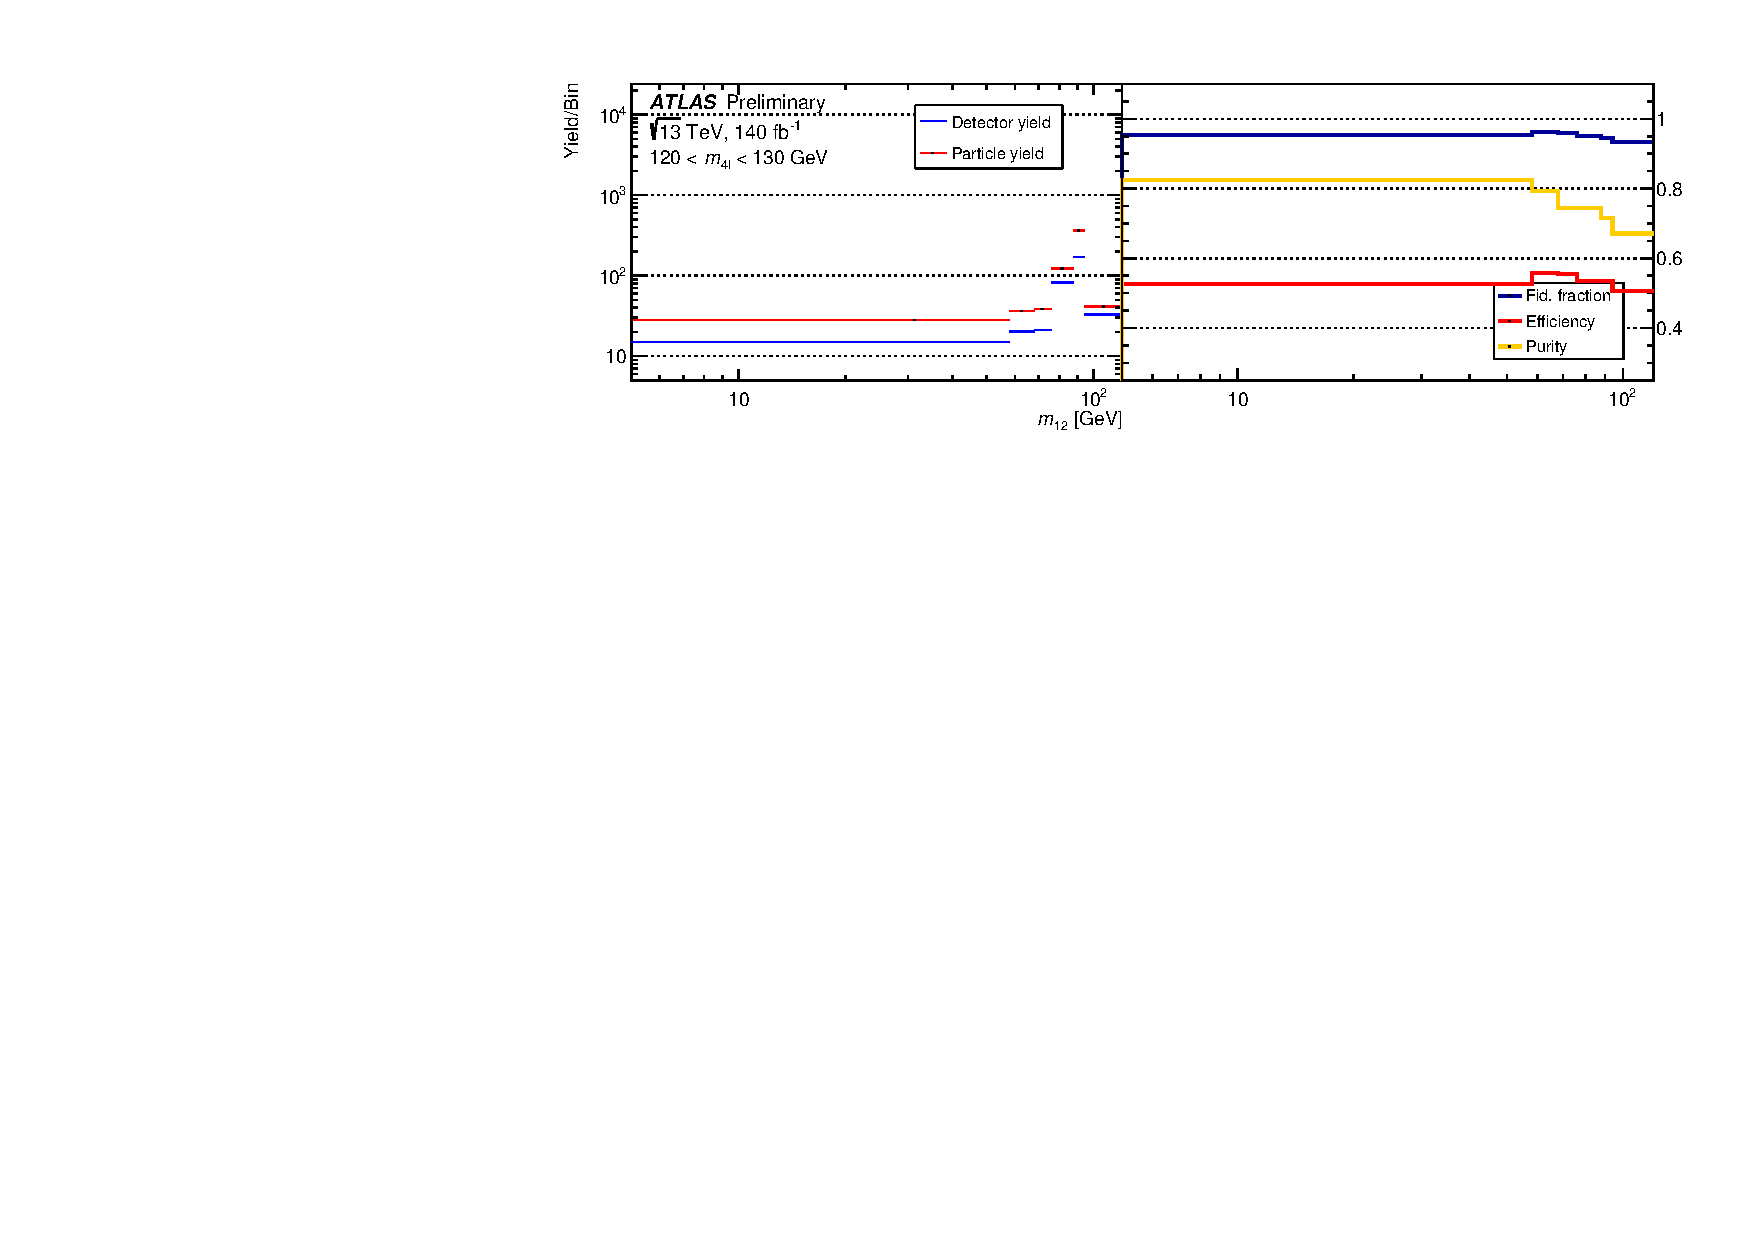
\includegraphics[width = 0.75\textwidth]{figures/UnfoldingStudies/v014_inputs/m12_m4l120-130inputs.pdf}}\\
  \subfigure{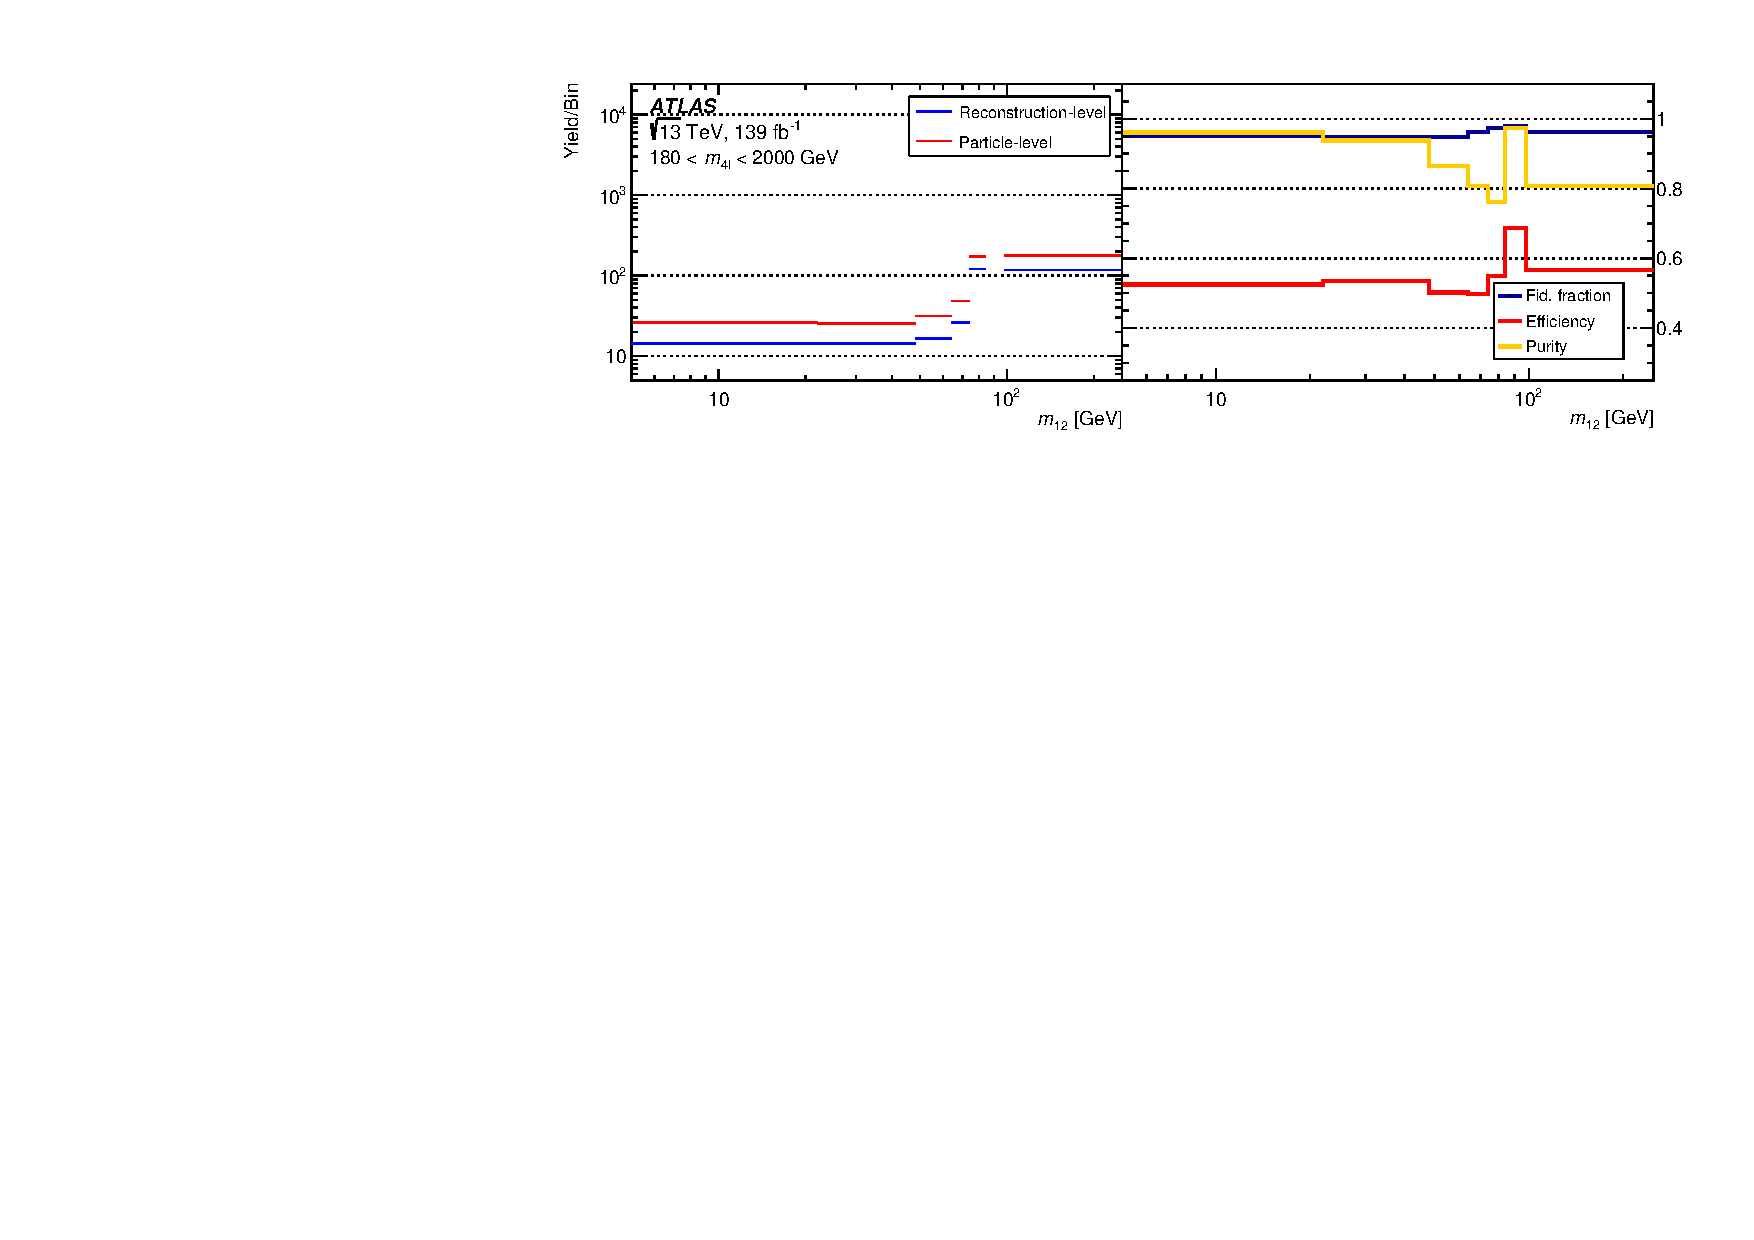
\includegraphics[width = 0.75\textwidth]{figures/UnfoldingStudies/v014_inputs/m12_m4l180-2000inputs.pdf}}\\
  \subfigure{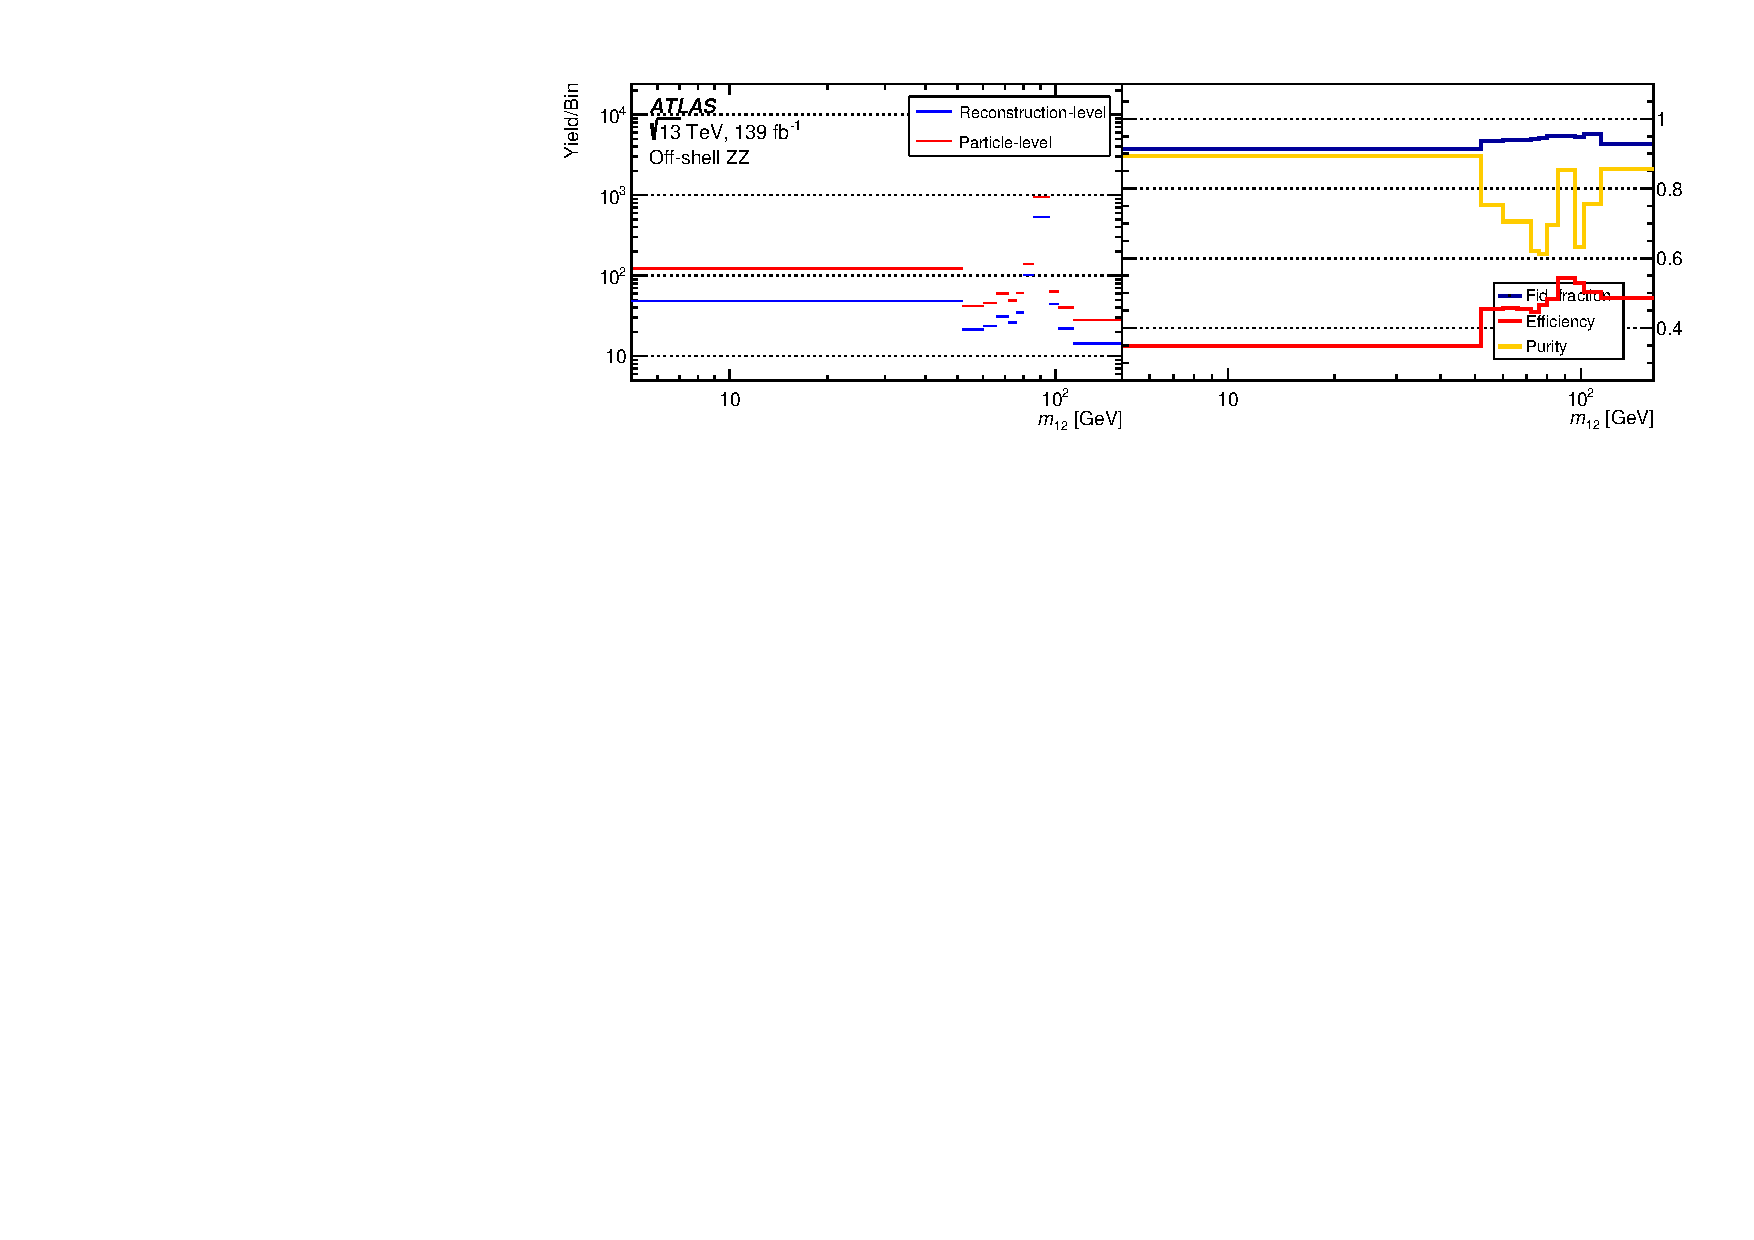
\includegraphics[width = 0.75\textwidth]{figures/UnfoldingStudies/v014_inputs/m12_m4loffshellinputs.pdf}}\\
\caption{In the left-hand panels, the number of predicted events passing the reconstruction- and fiducial- level selections are displayed as the detector yield and particle yield, respectively. The right-hand panel shows the efficiency, fiducial purity and fiducial fraction. All variables are plotted as a function of the \mZOne bins, in slices of the \mFourL variable which are stacked and labelled with the included \mFourL range.
  \label{fig:mZ1unf}}
 \end{figure}  


\FloatBarrier
\clearpage
\begin{figure}[htb]
  \centering 
  \subfigure{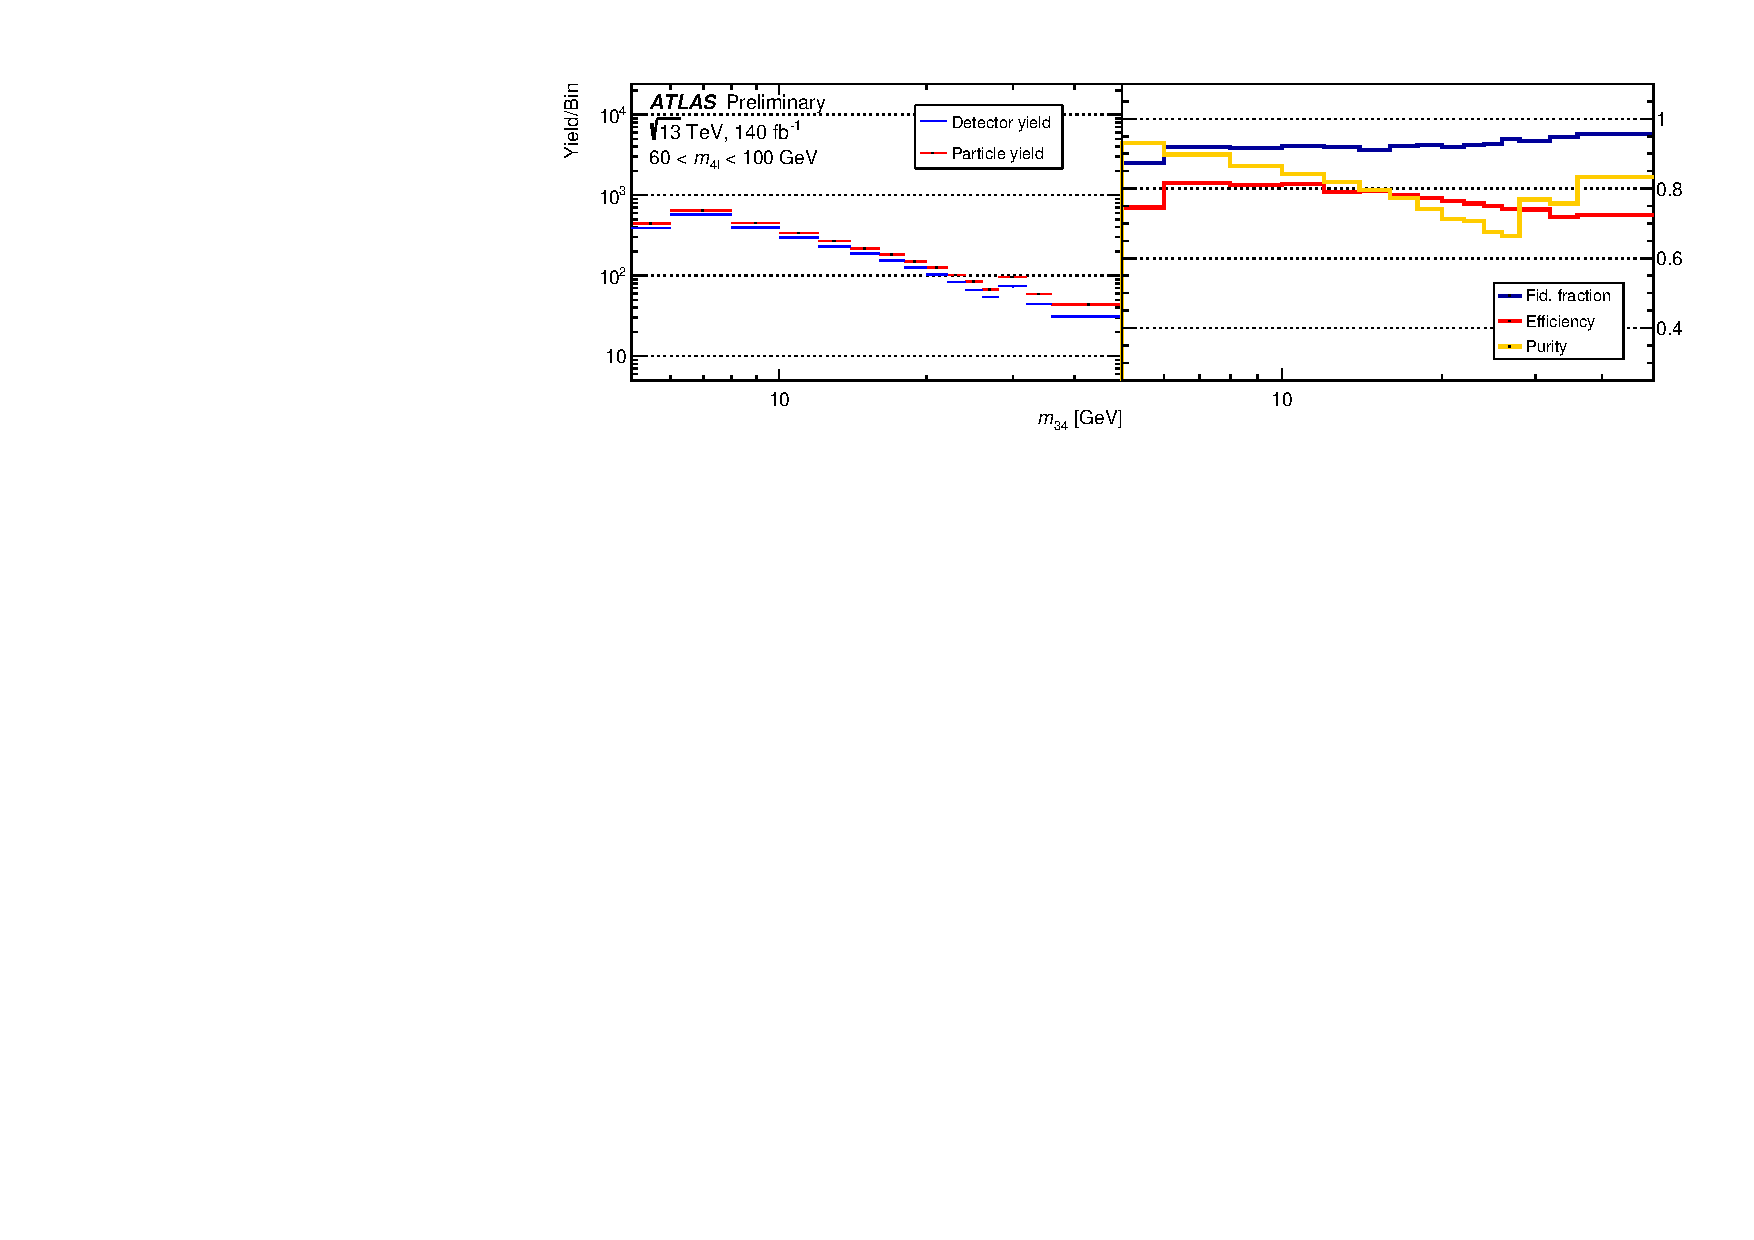
\includegraphics[width = 0.75\textwidth]{figures/UnfoldingStudies/v014_inputs/m34_m4l60-100inputs.pdf}}\\
  \subfigure{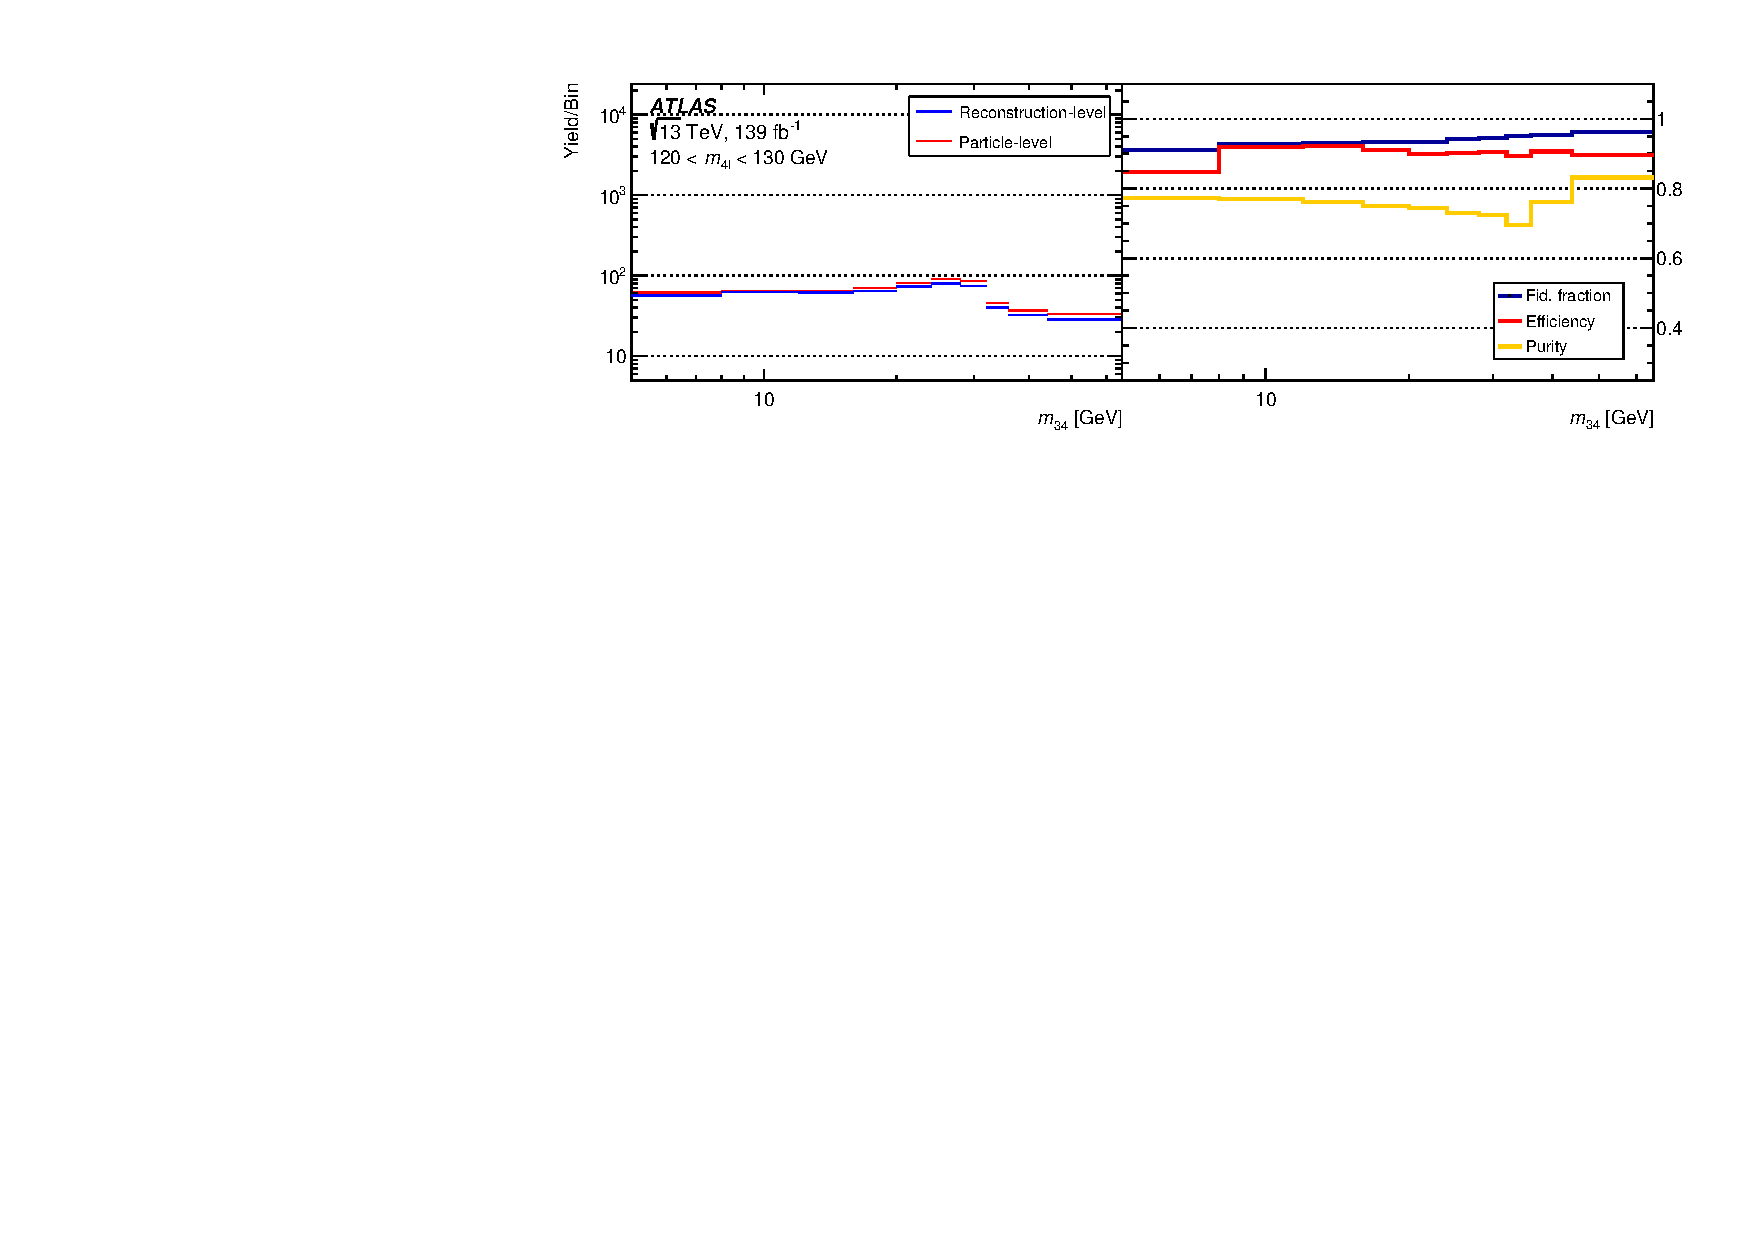
\includegraphics[width = 0.75\textwidth]{figures/UnfoldingStudies/v014_inputs/m34_m4l120-130inputs.pdf}}\\
  \subfigure{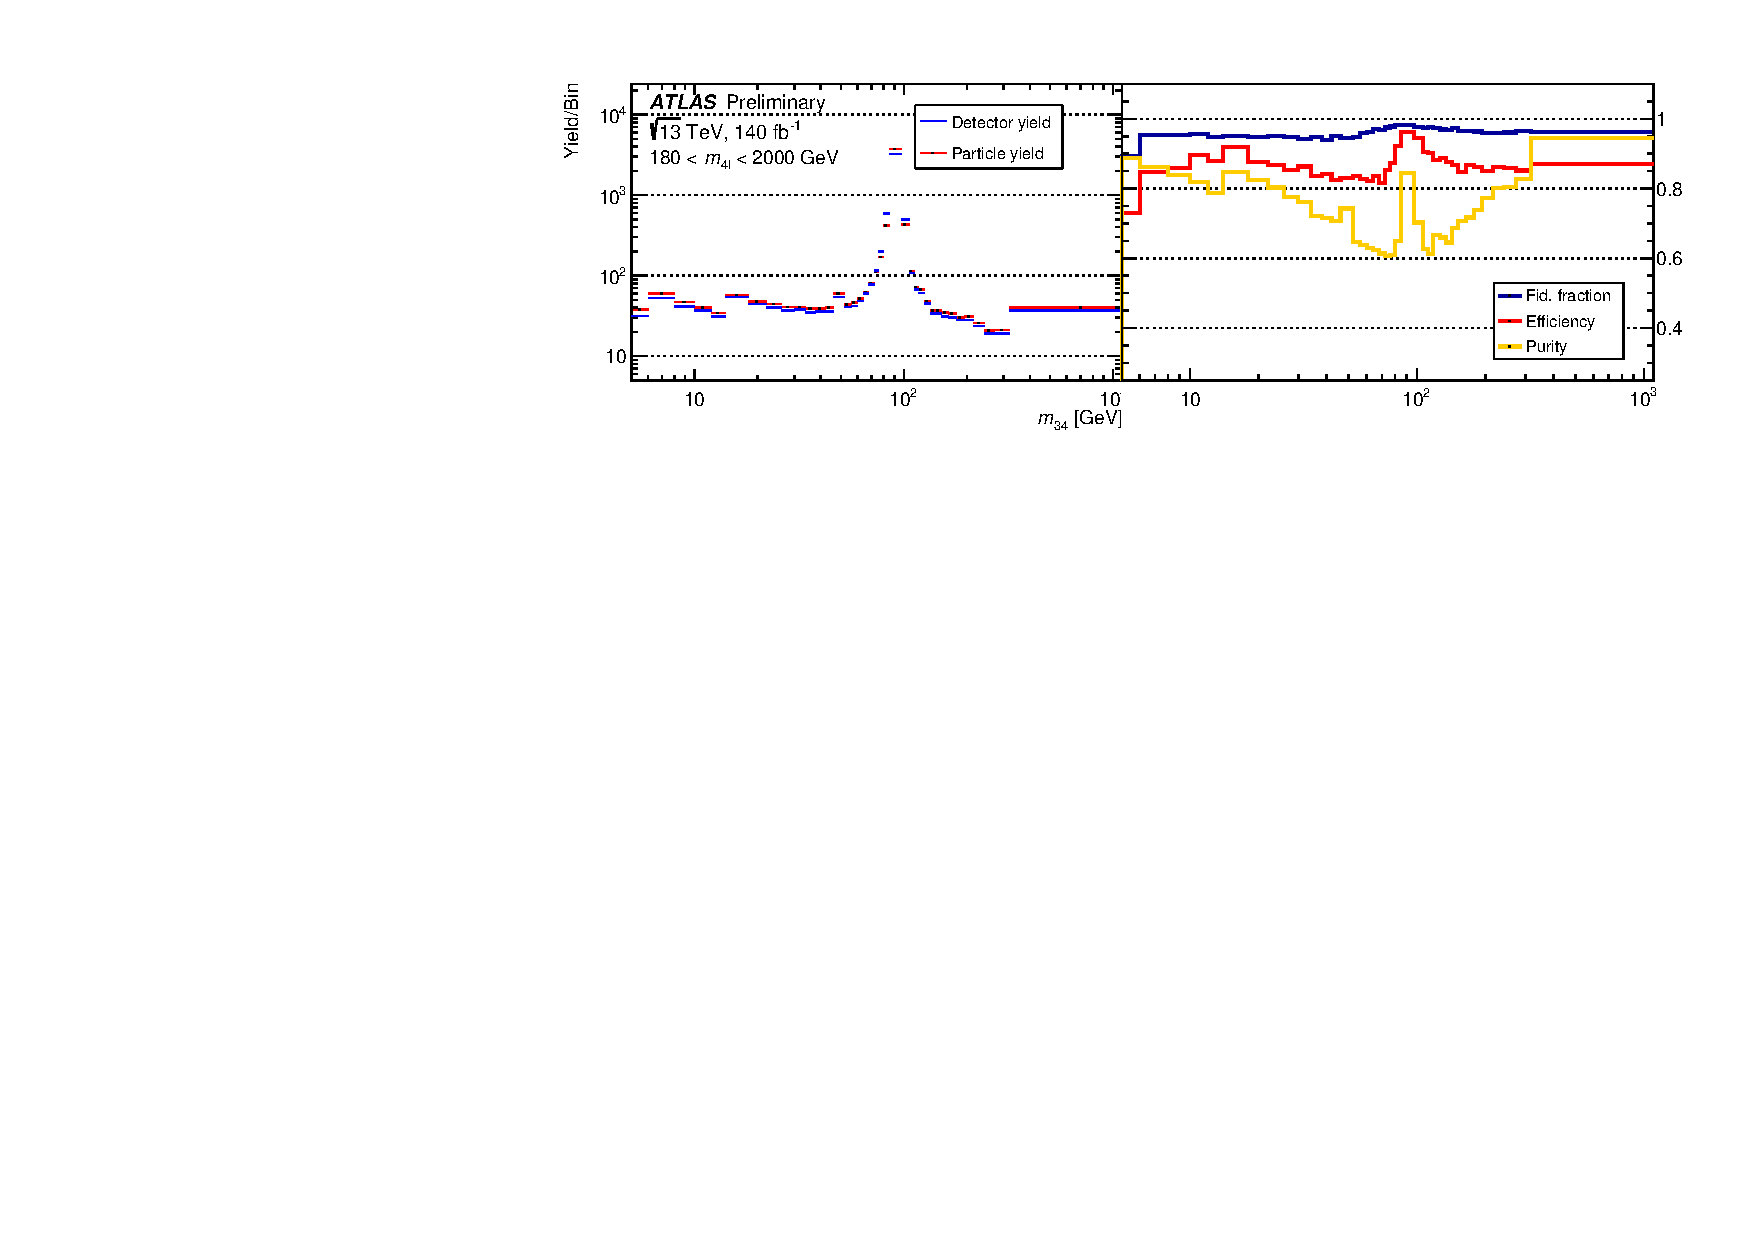
\includegraphics[width = 0.75\textwidth]{figures/UnfoldingStudies/v014_inputs/m34_m4l180-2000inputs.pdf}}\\
  \subfigure{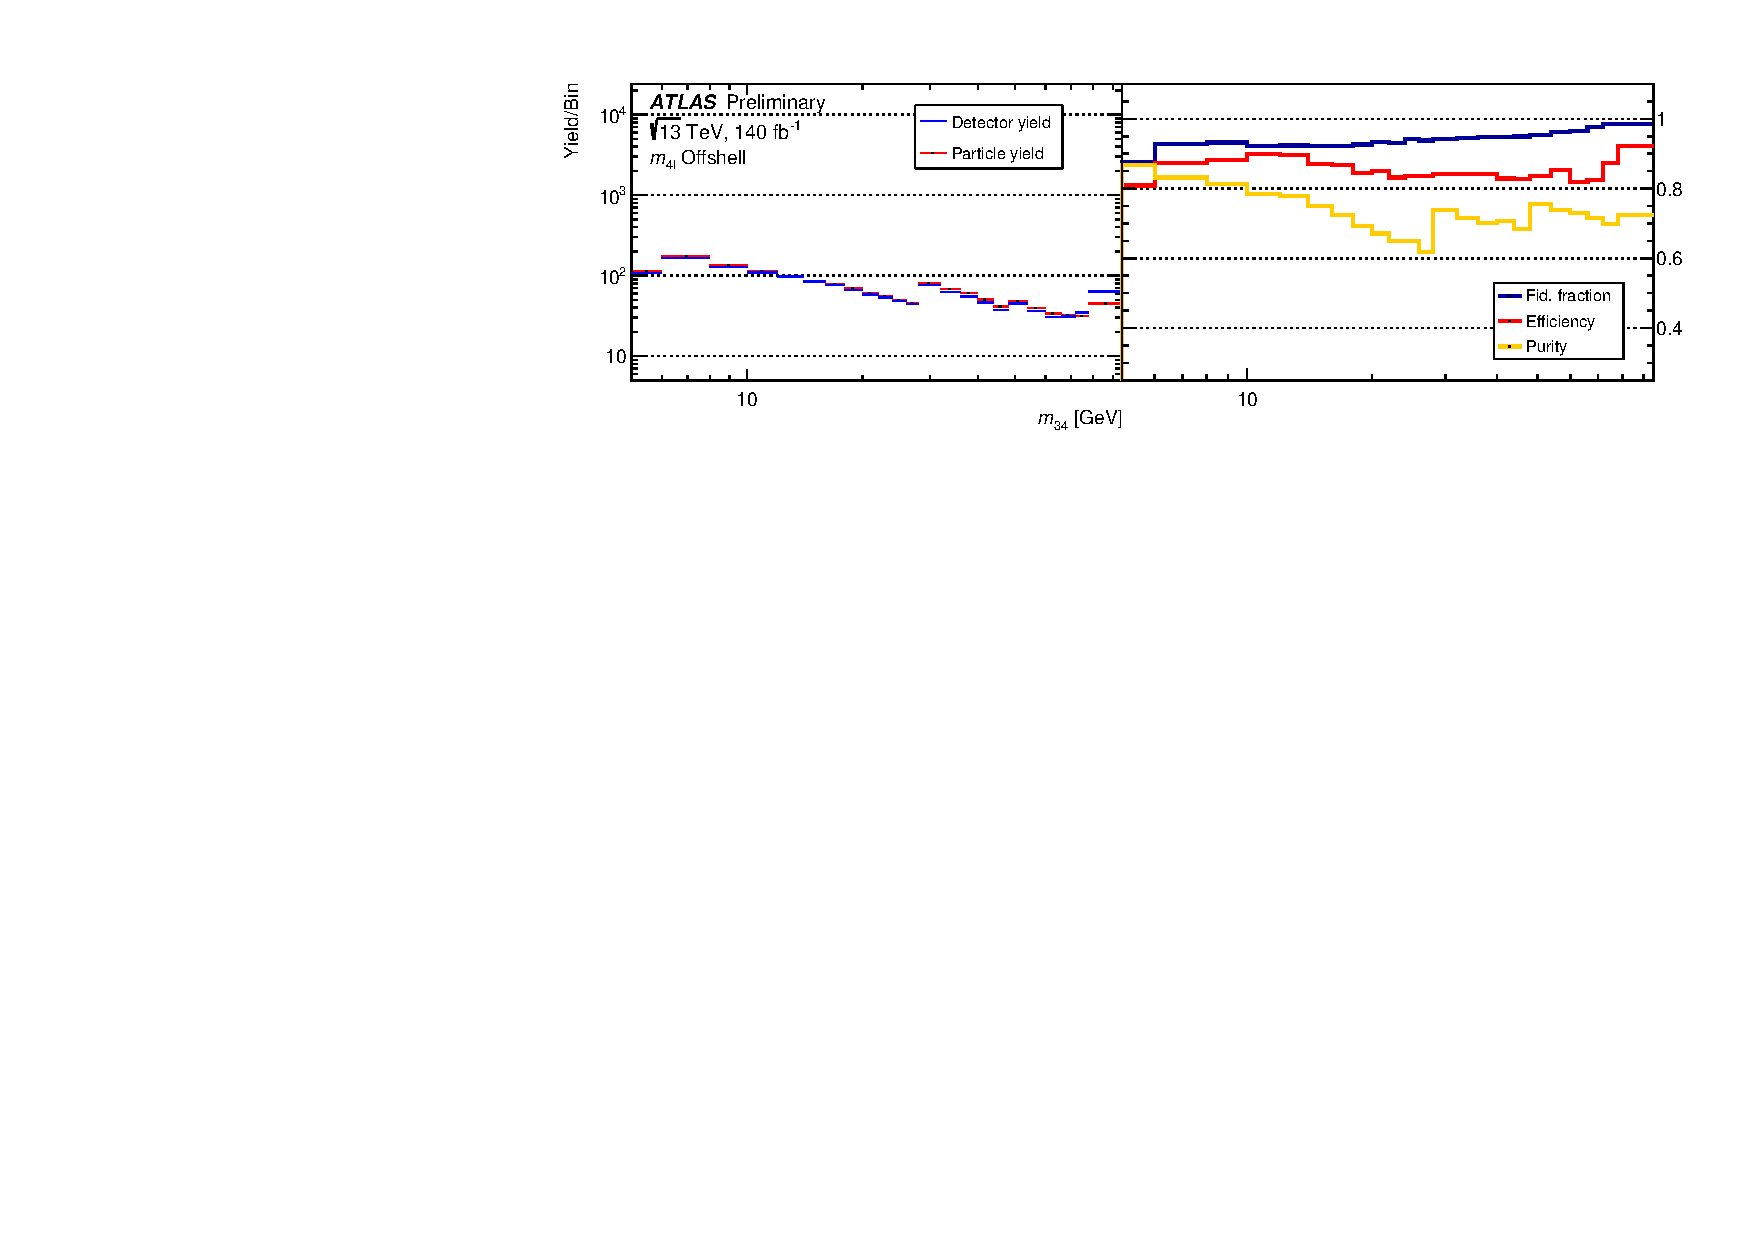
\includegraphics[width = 0.75\textwidth]{figures/UnfoldingStudies/v014_inputs/m34_m4loffshellinputs.pdf}}\\
\caption{In the left-hand panels, the number of predicted events passing the reconstruction- and fiducial- level selections are displayed as the detector yield and particle yield, respectively. The right-hand panel shows the efficiency, fiducial purity and fiducial fraction. All variables are plotted as a function of the \mZTwo bins, in slices of the \mFourL variable which are stacked and labelled with the included \mFourL range.
  \label{fig:mZ2unf}}
 \end{figure}  



\FloatBarrier
\clearpage

\begin{figure}[htb]
  \centering 
  \subfigure{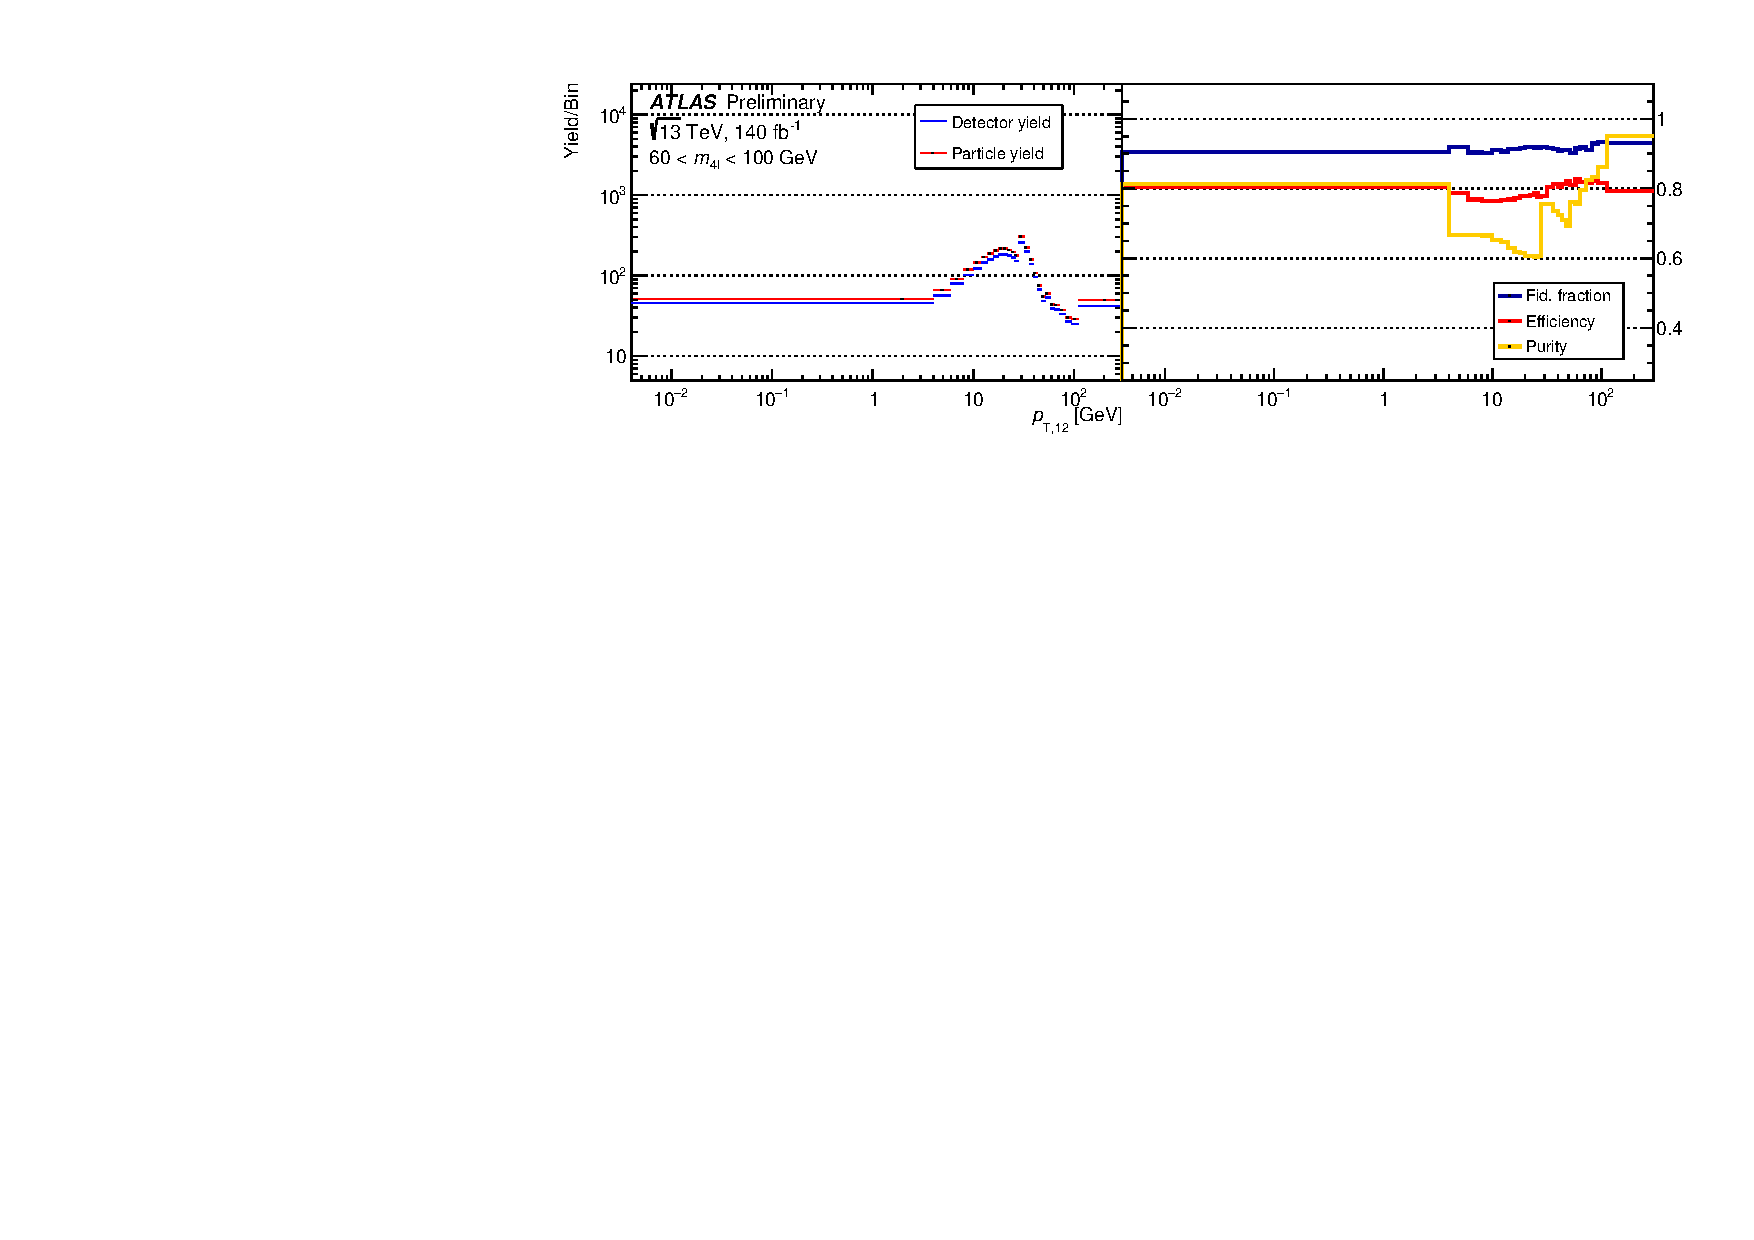
\includegraphics[width = 0.75\textwidth]{figures/UnfoldingStudies/v014_inputs/pt12_m4l60-100inputs.pdf}}\\
  \subfigure{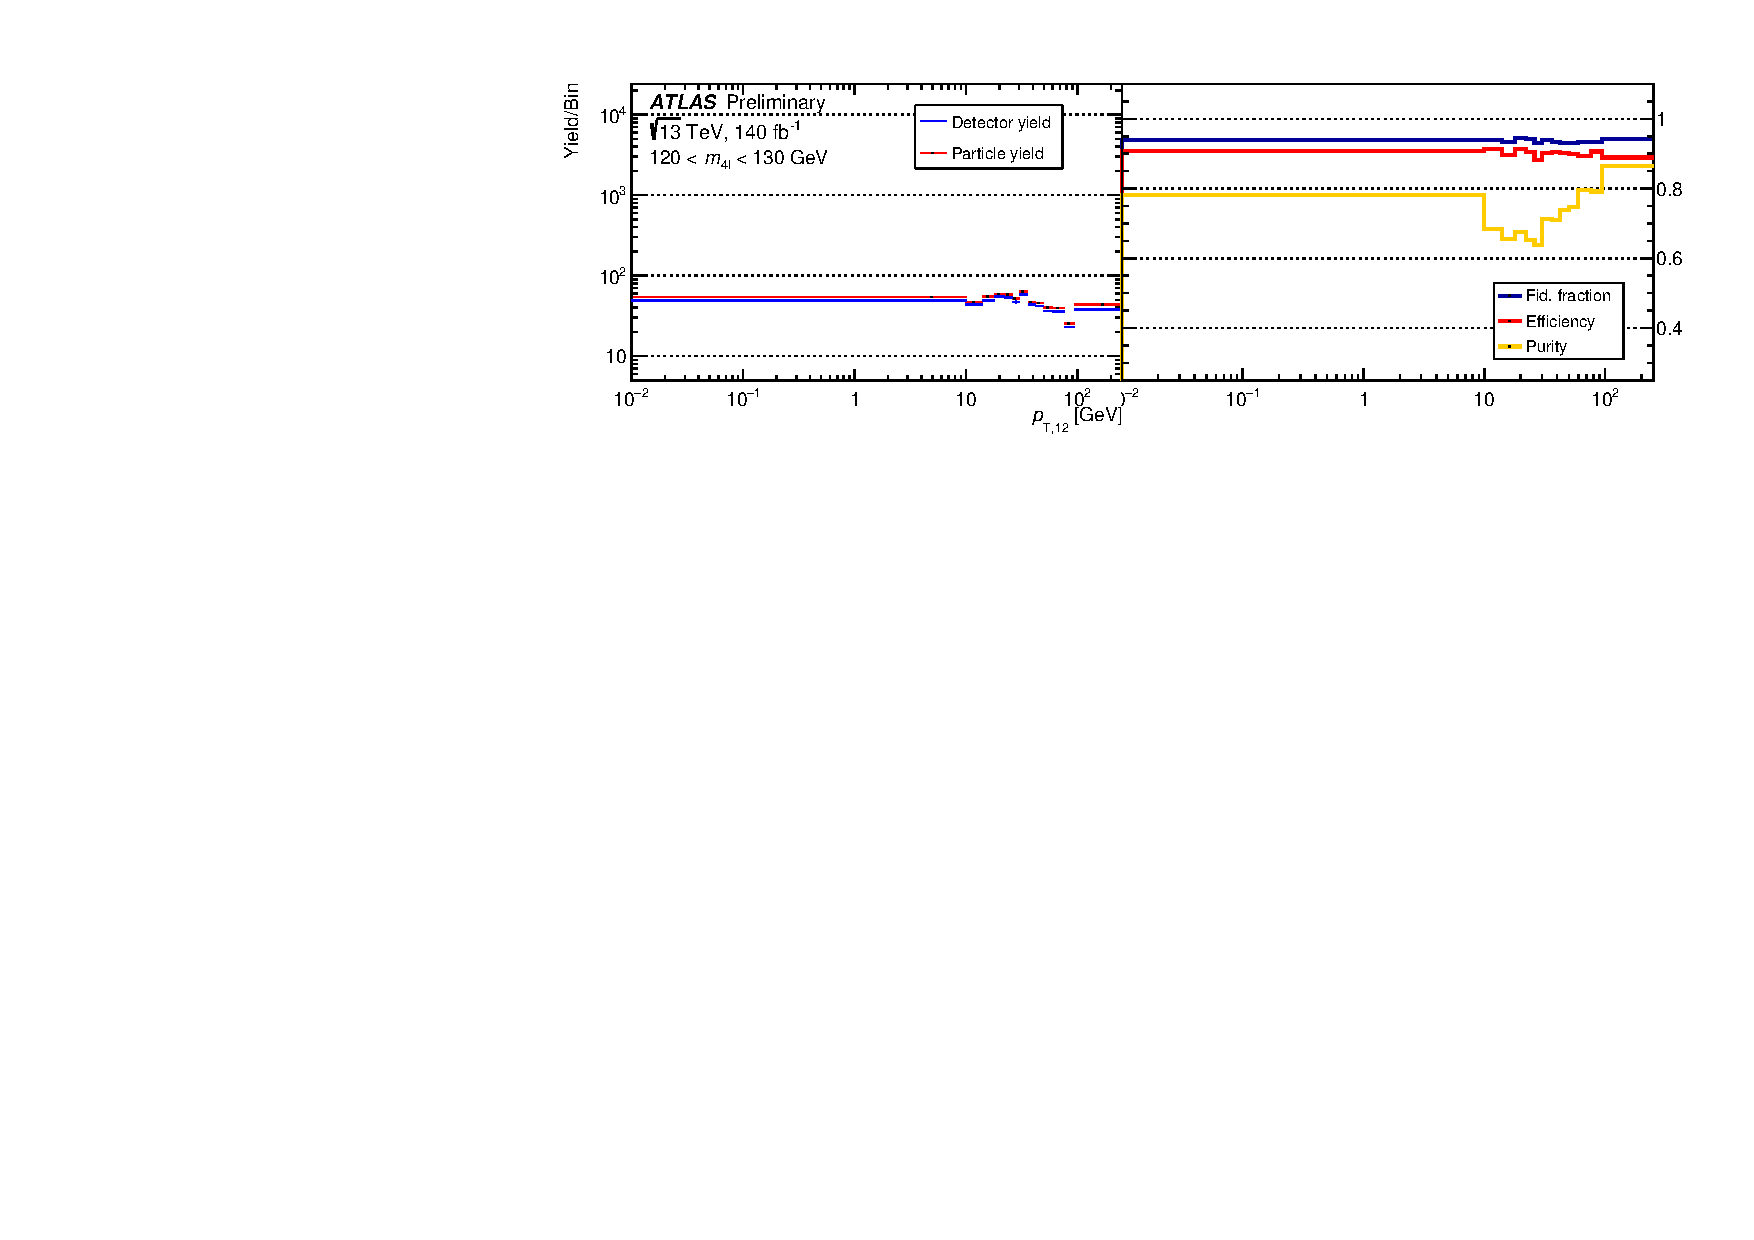
\includegraphics[width = 0.75\textwidth]{figures/UnfoldingStudies/v014_inputs/pt12_m4l120-130inputs.pdf}}\\
  \subfigure{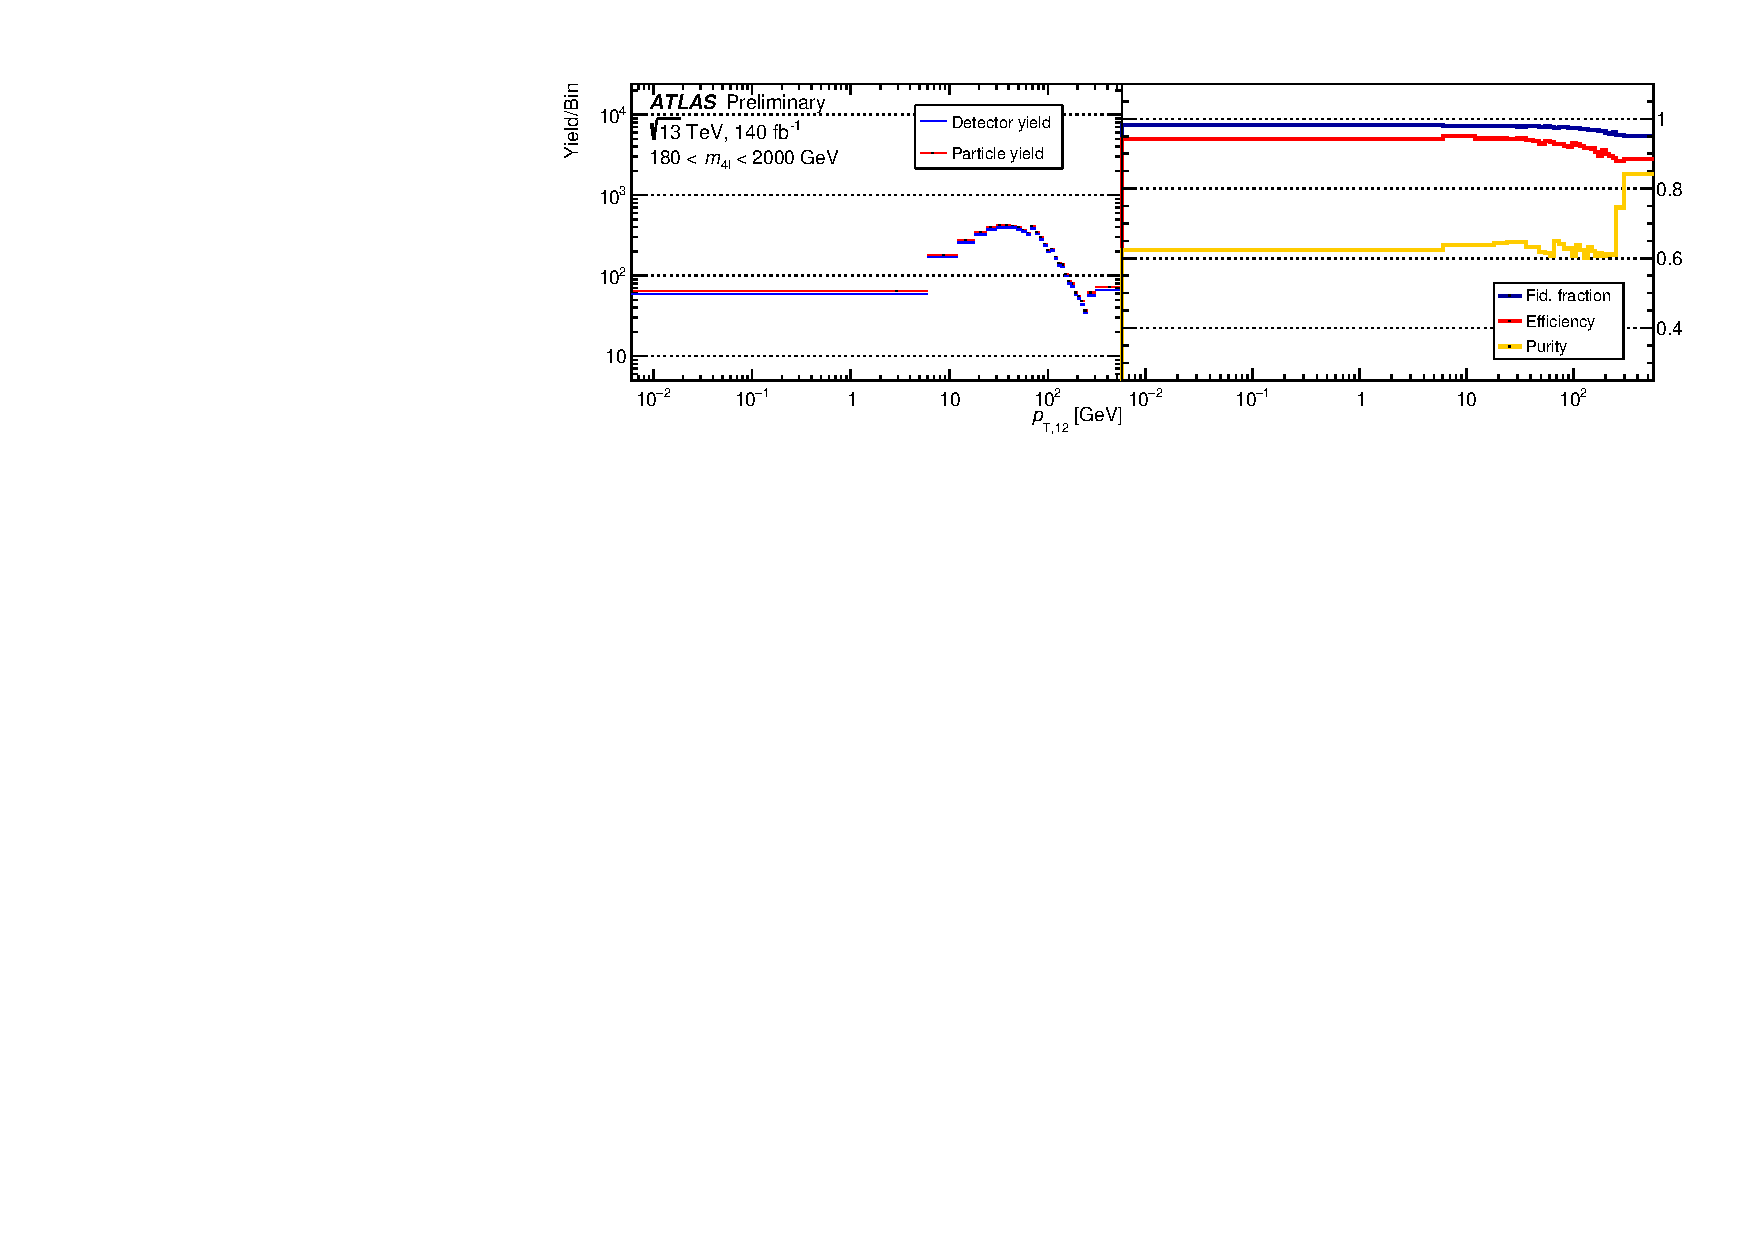
\includegraphics[width = 0.75\textwidth]{figures/UnfoldingStudies/v014_inputs/pt12_m4l180-2000inputs.pdf}}\\
  \subfigure{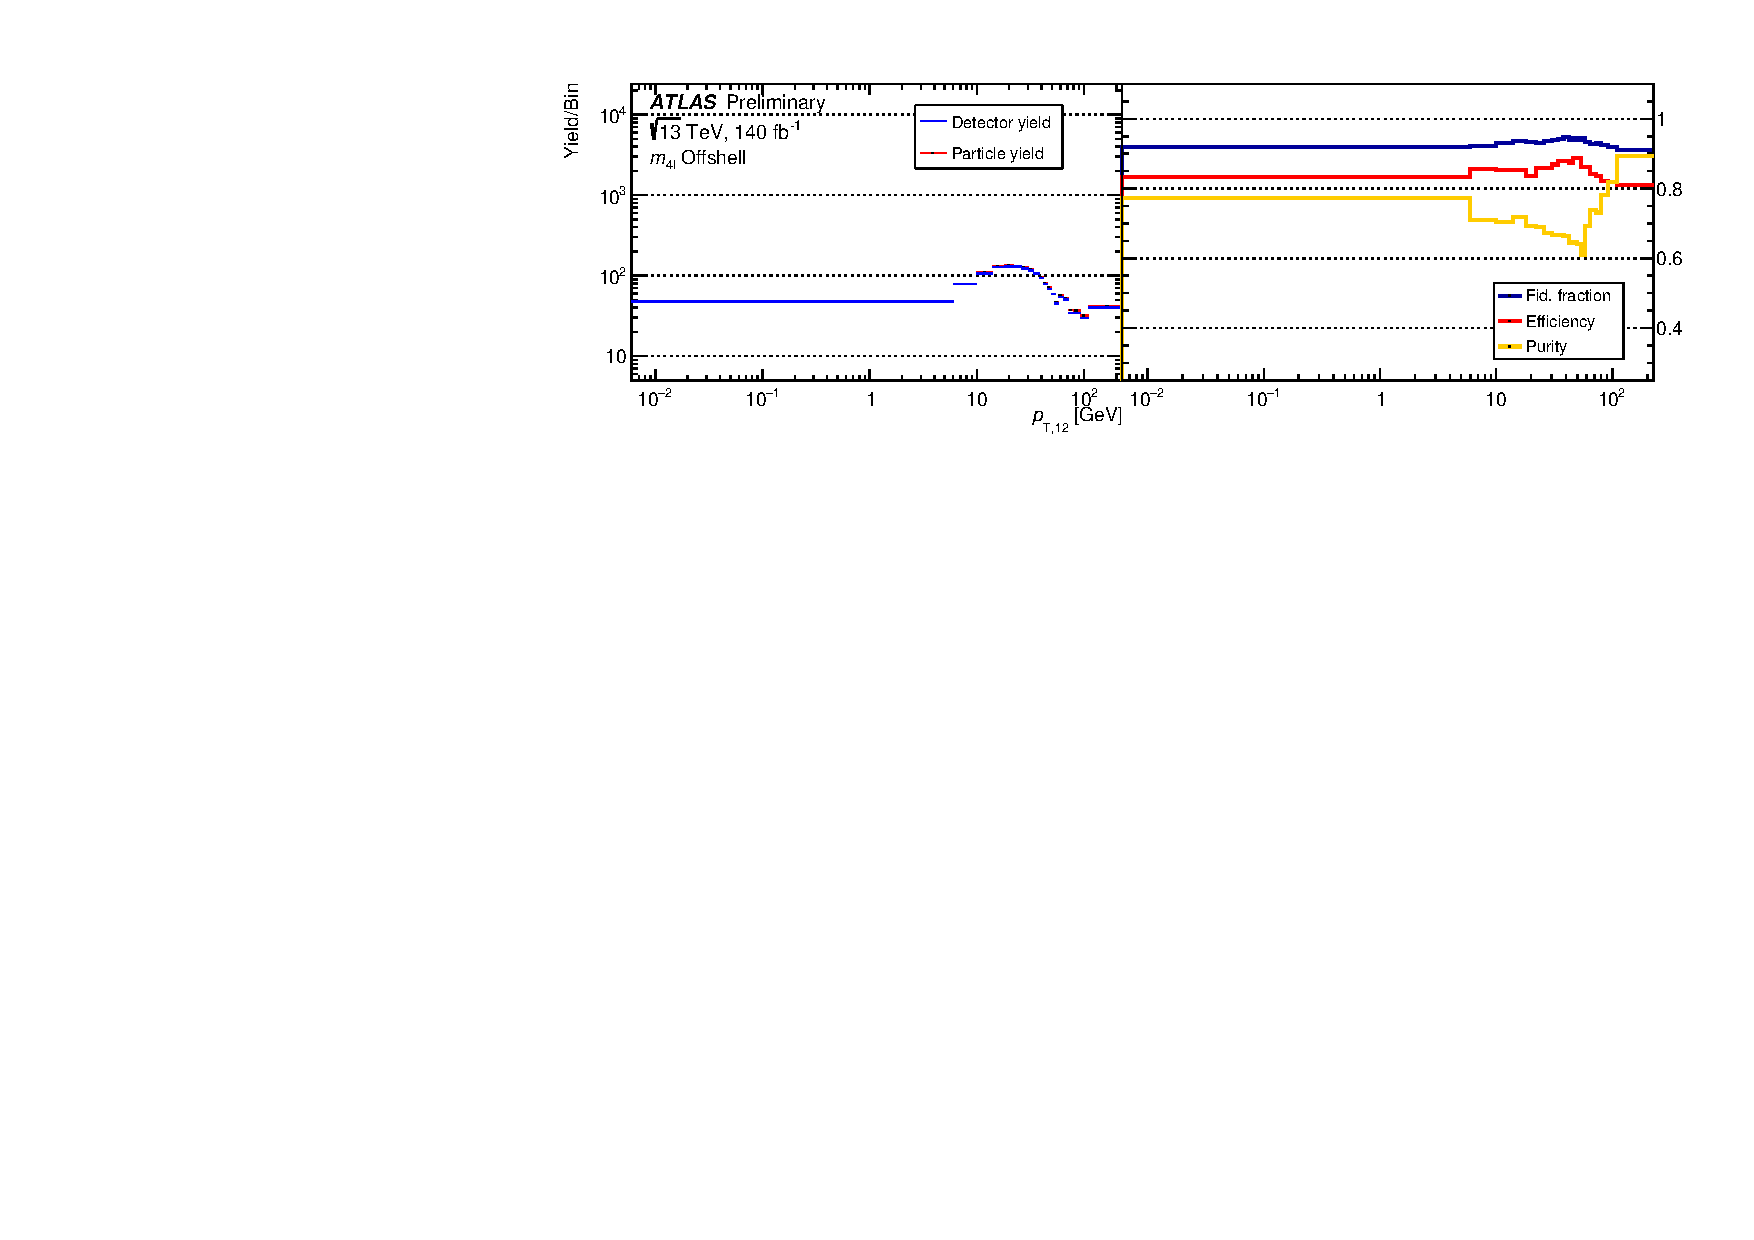
\includegraphics[width = 0.75\textwidth]{figures/UnfoldingStudies/v014_inputs/pt12_m4loffshellinputs.pdf}}\\
\caption{In the left-hand panels, the number of predicted events passing the reconstruction- and fiducial- level selections are displayed as the detector yield and particle yield, respectively. The right-hand panel shows the efficiency, fiducial purity and fiducial fraction. All variables are plotted as a function of the \ptZOne bins, in slices of the \mFourL variable which are stacked and labelled with the included \mFourL range.
  \label{fig:ptZ1unf}}
 \end{figure}  


\FloatBarrier
\clearpage

\begin{figure}[htb]
  \centering 
  \subfigure{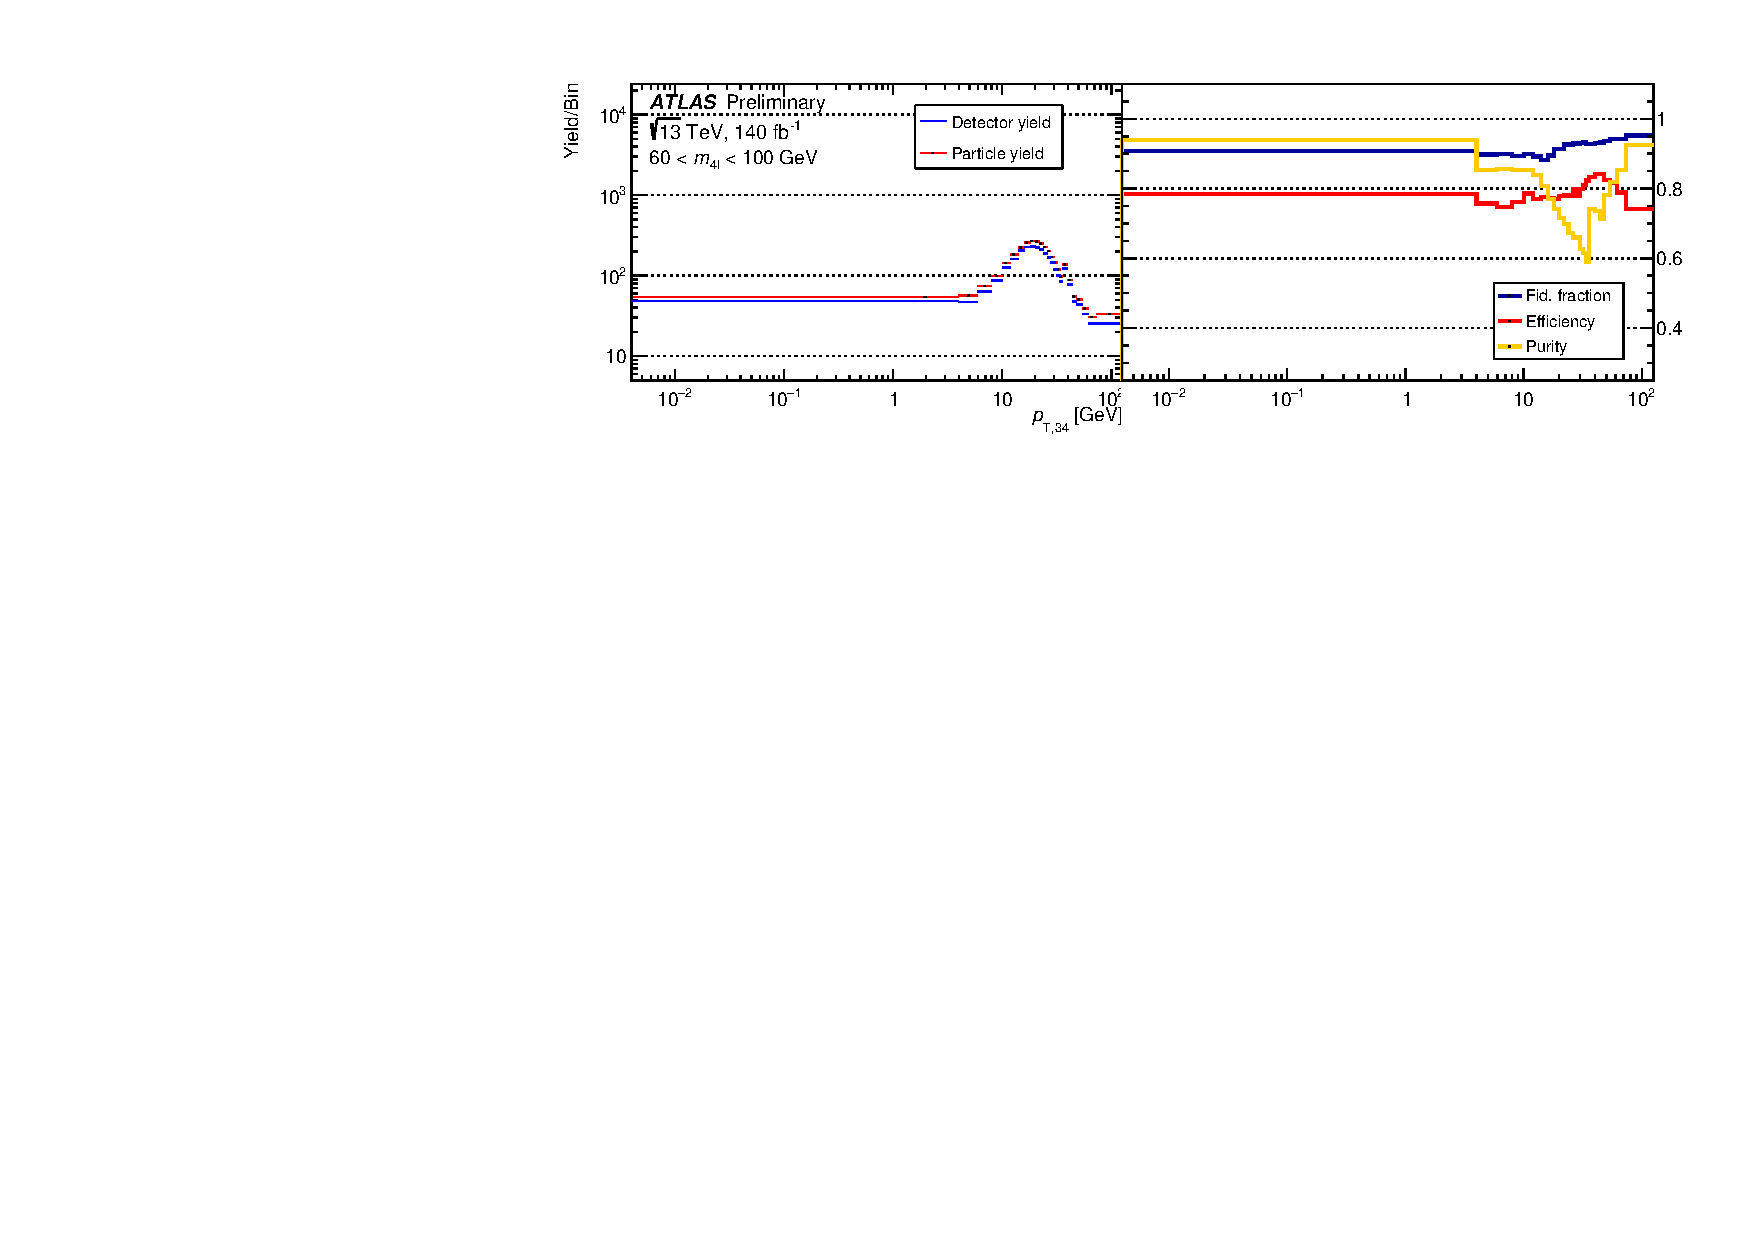
\includegraphics[width = 0.75\textwidth]{figures/UnfoldingStudies/v014_inputs/pt34_m4l60-100inputs.pdf}}\\
  \subfigure{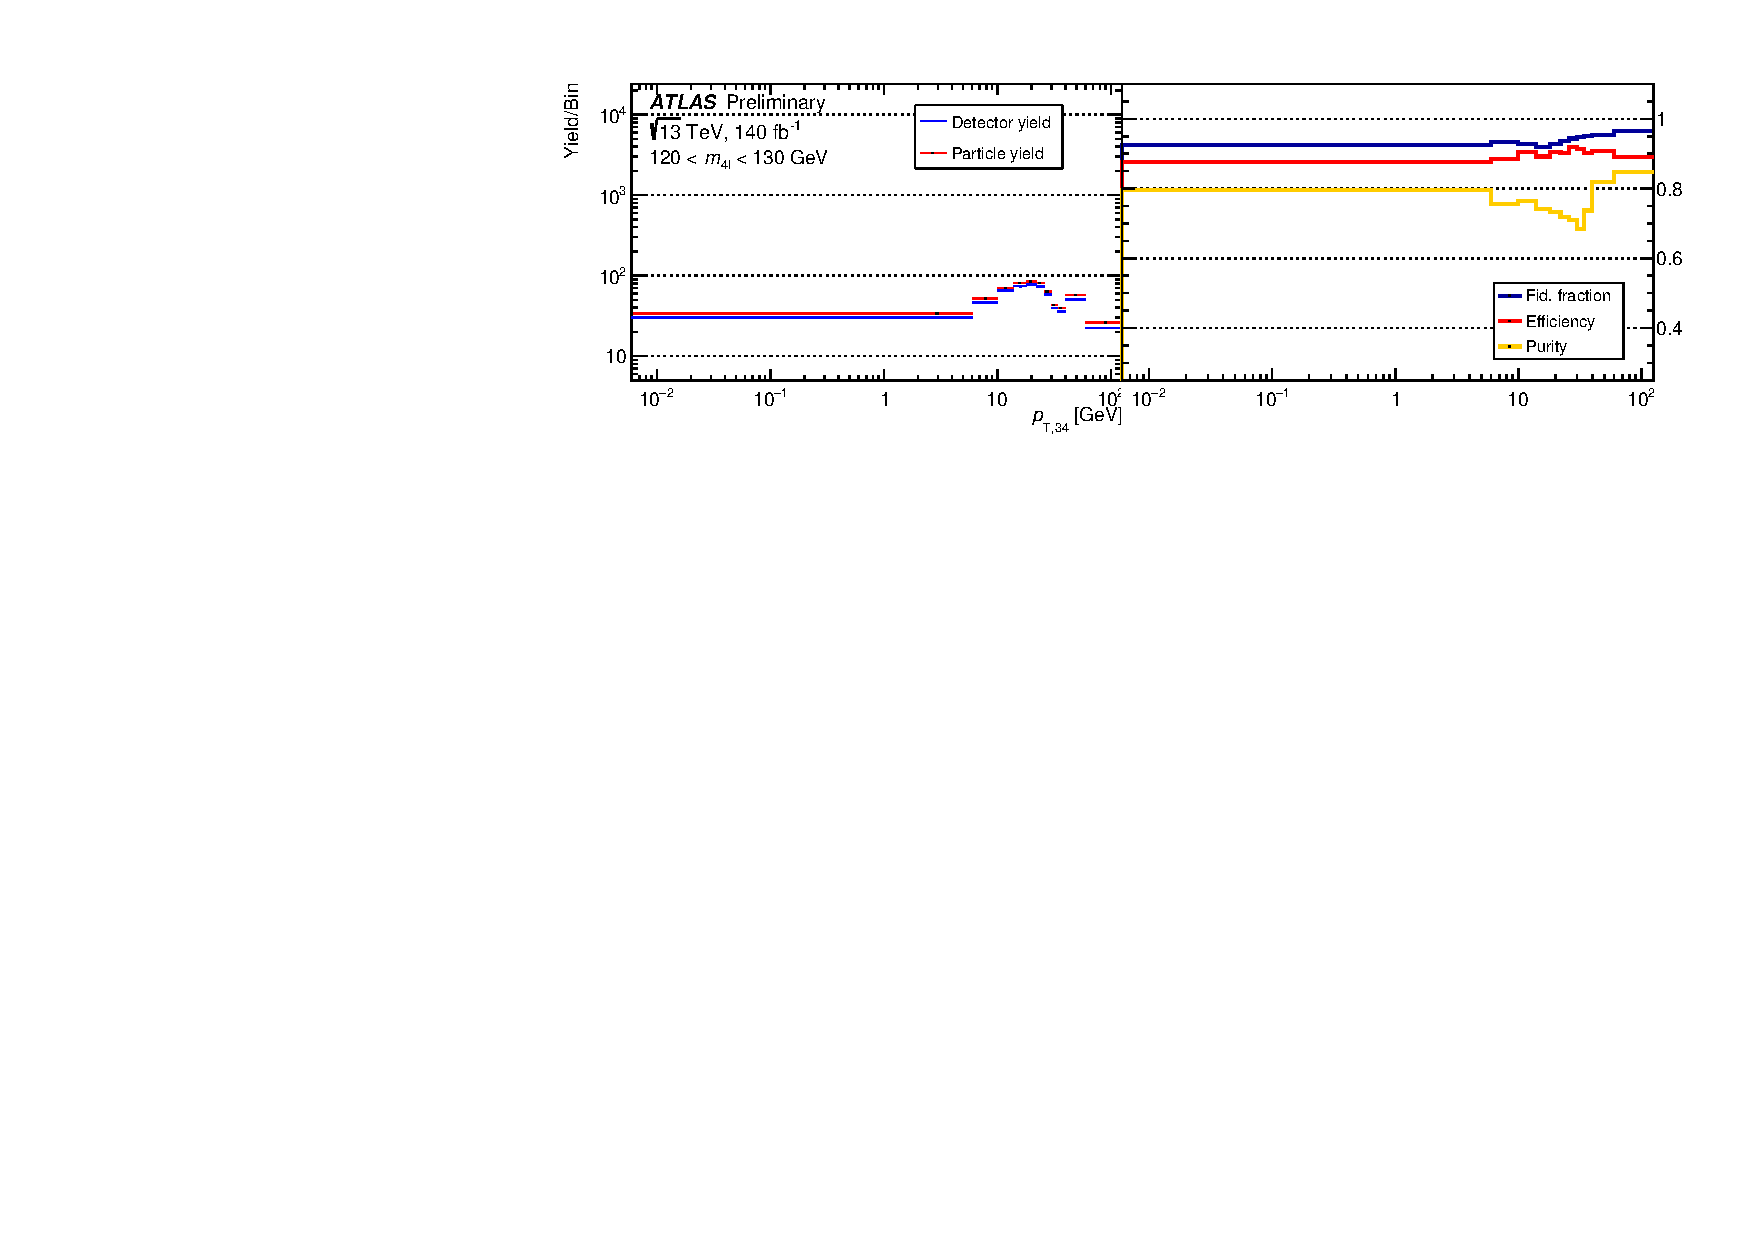
\includegraphics[width = 0.75\textwidth]{figures/UnfoldingStudies/v014_inputs/pt34_m4l120-130inputs.pdf}}\\
  \subfigure{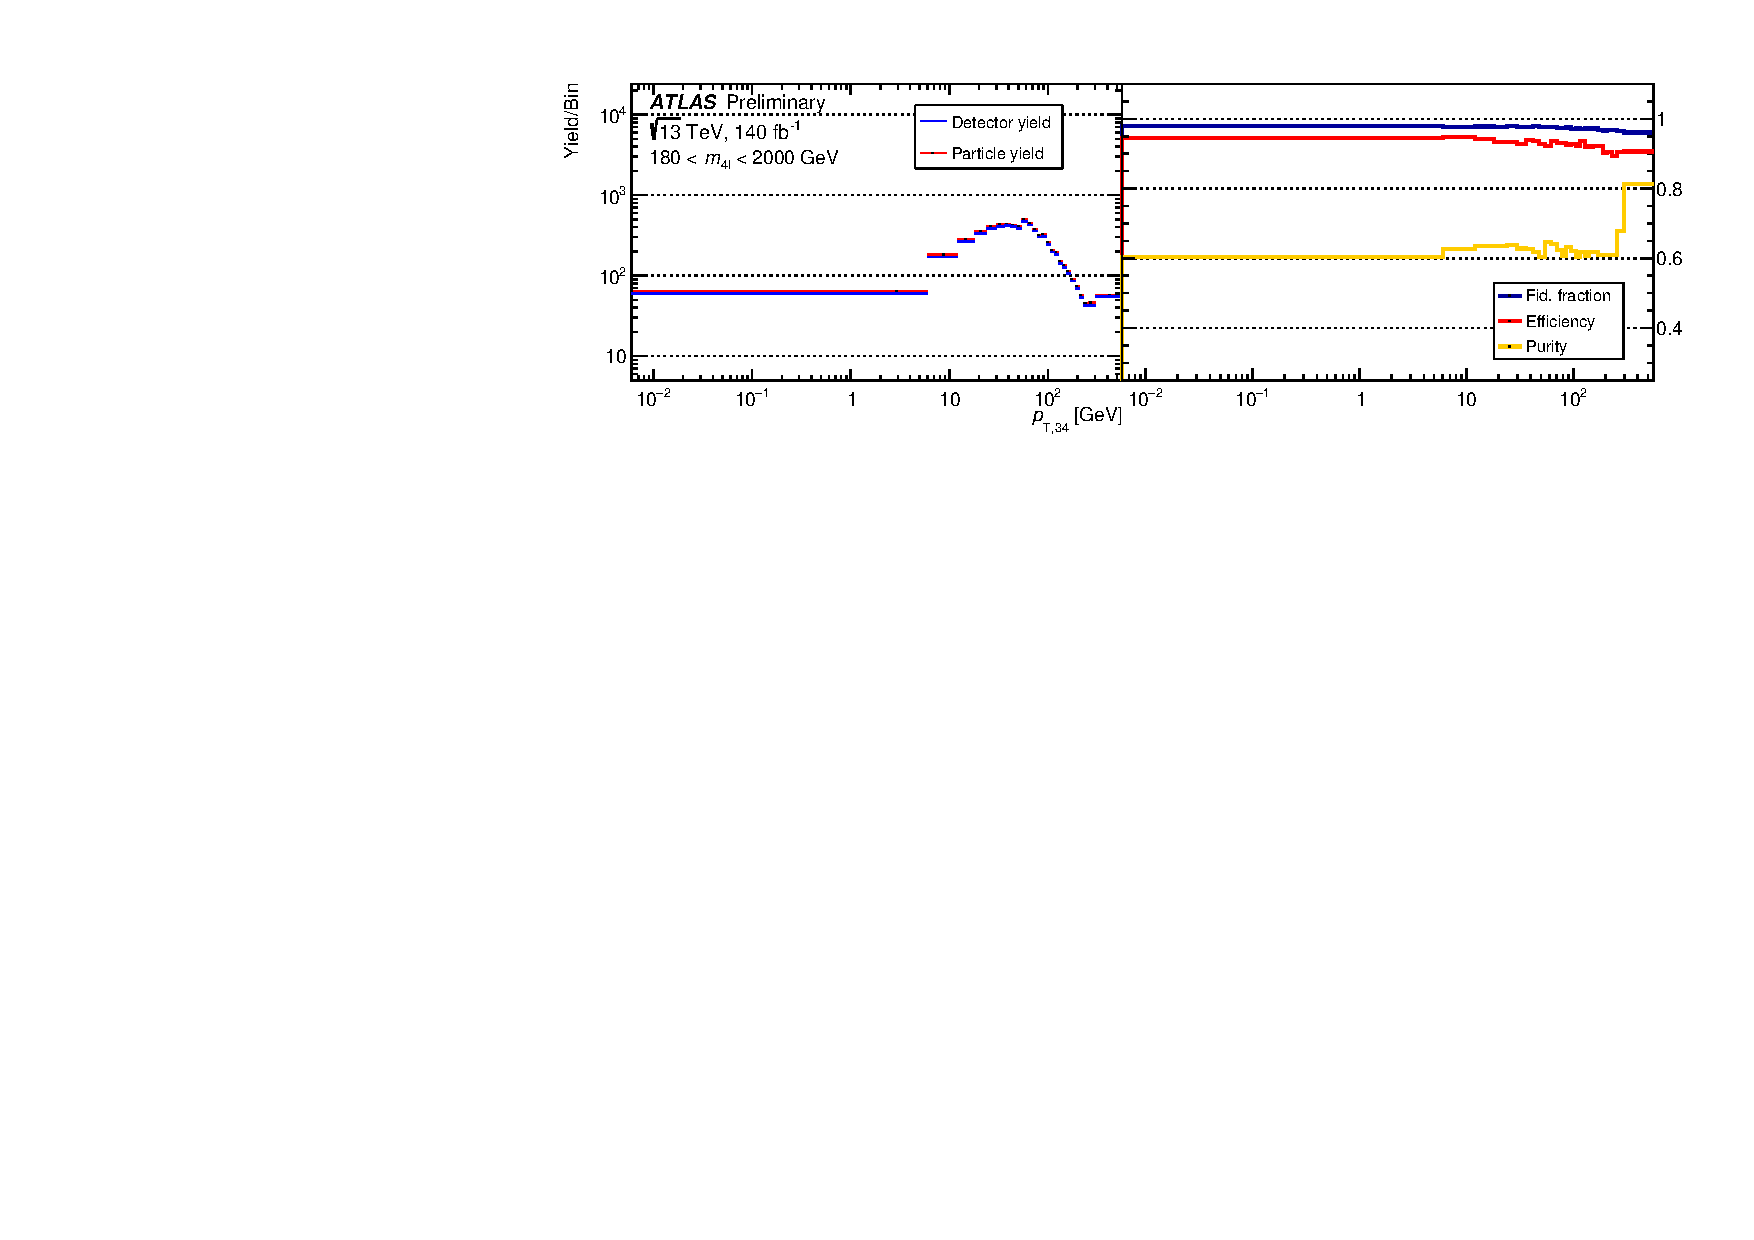
\includegraphics[width = 0.75\textwidth]{figures/UnfoldingStudies/v014_inputs/pt34_m4l180-2000inputs.pdf}}\\
  \subfigure{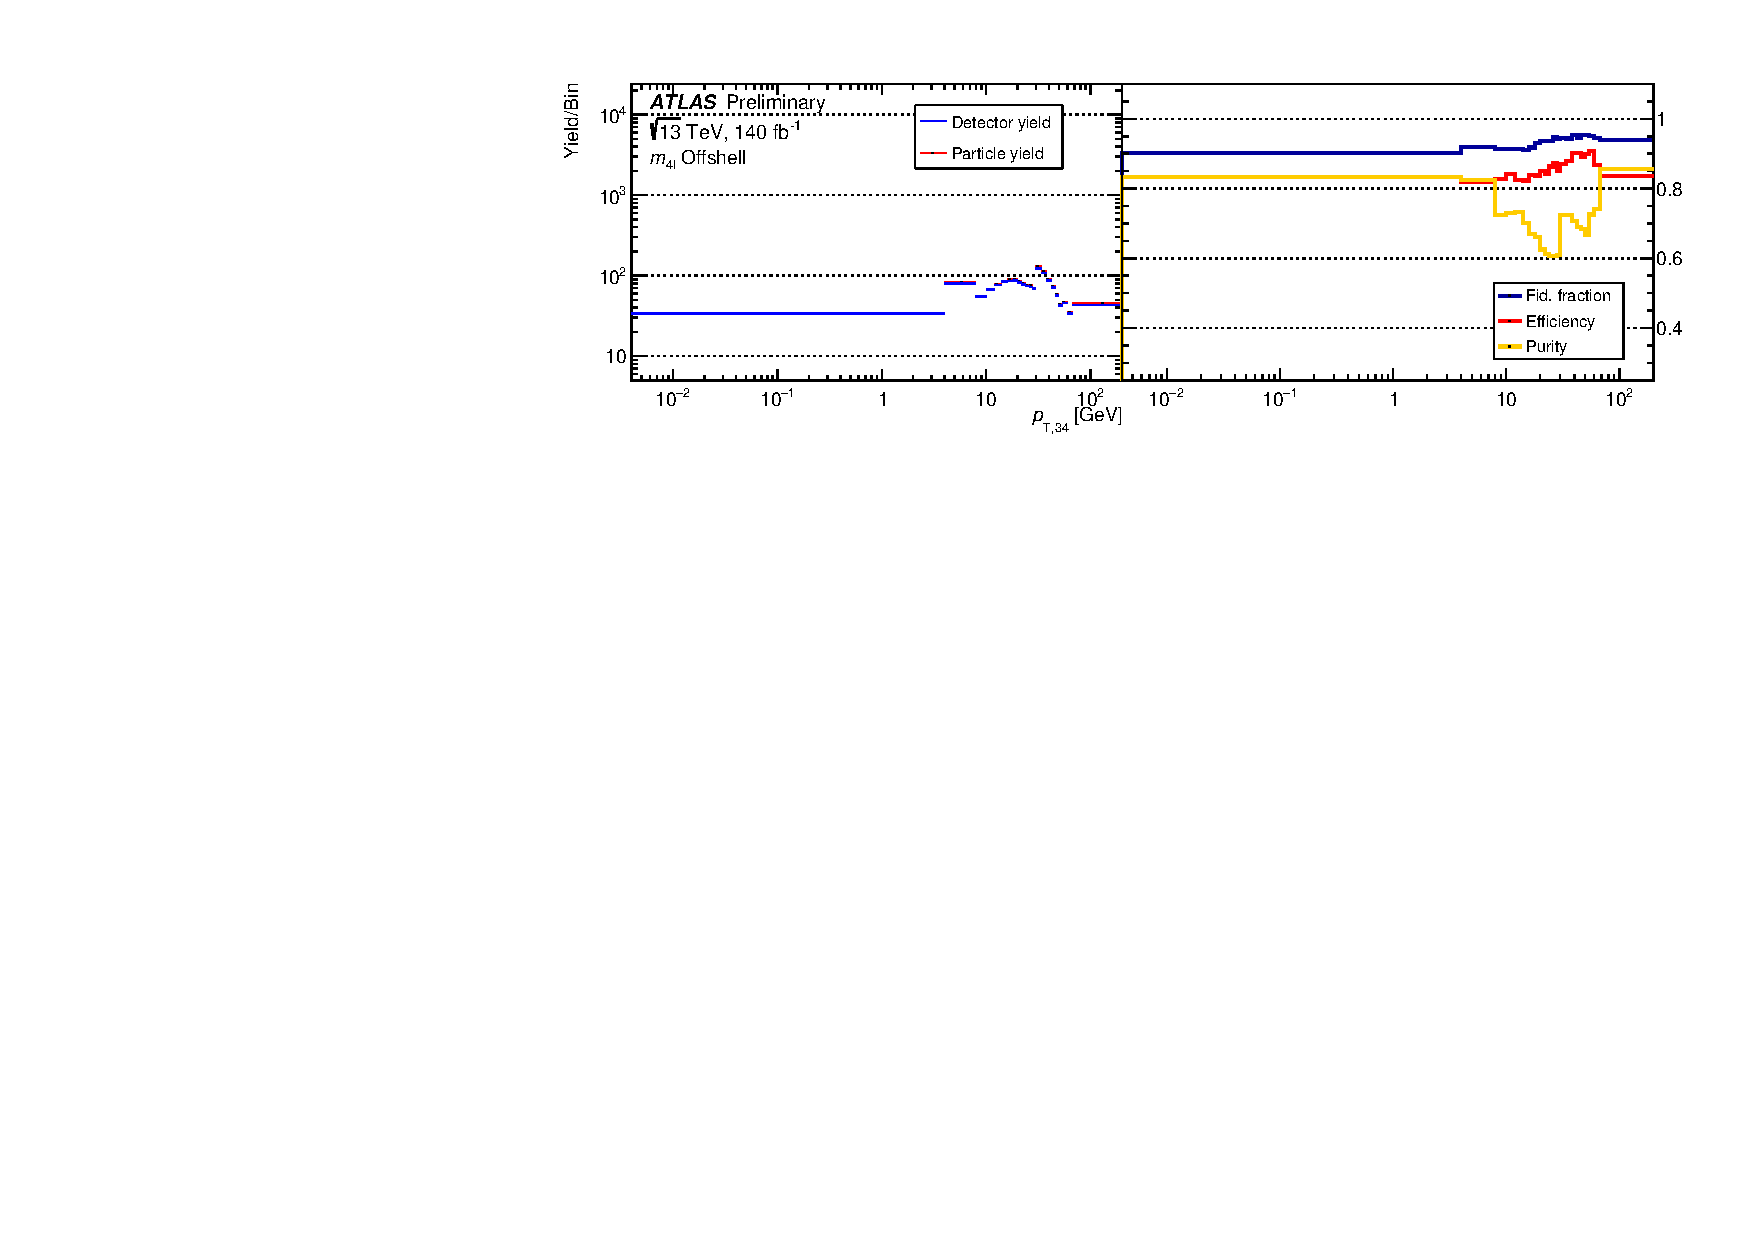
\includegraphics[width = 0.75\textwidth]{figures/UnfoldingStudies/v014_inputs/pt34_m4loffshellinputs.pdf}}\\
\caption{In the left-hand panels, the number of predicted events passing the reconstruction- and fiducial- level selections are displayed as the detector yield and particle yield, respectively. The right-hand panel shows the efficiency, fiducial purity and fiducial fraction. All variables are plotted as a function of the \ptZTwo bins, in slices of the \mFourL variable which are stacked and labelled with the included \mFourL range.
  \label{fig:ptZ2unf}}
 \end{figure}  


\FloatBarrier
\clearpage


%%All angular variables
\begin{figure}[htb]
  \centering 
  \subfigure{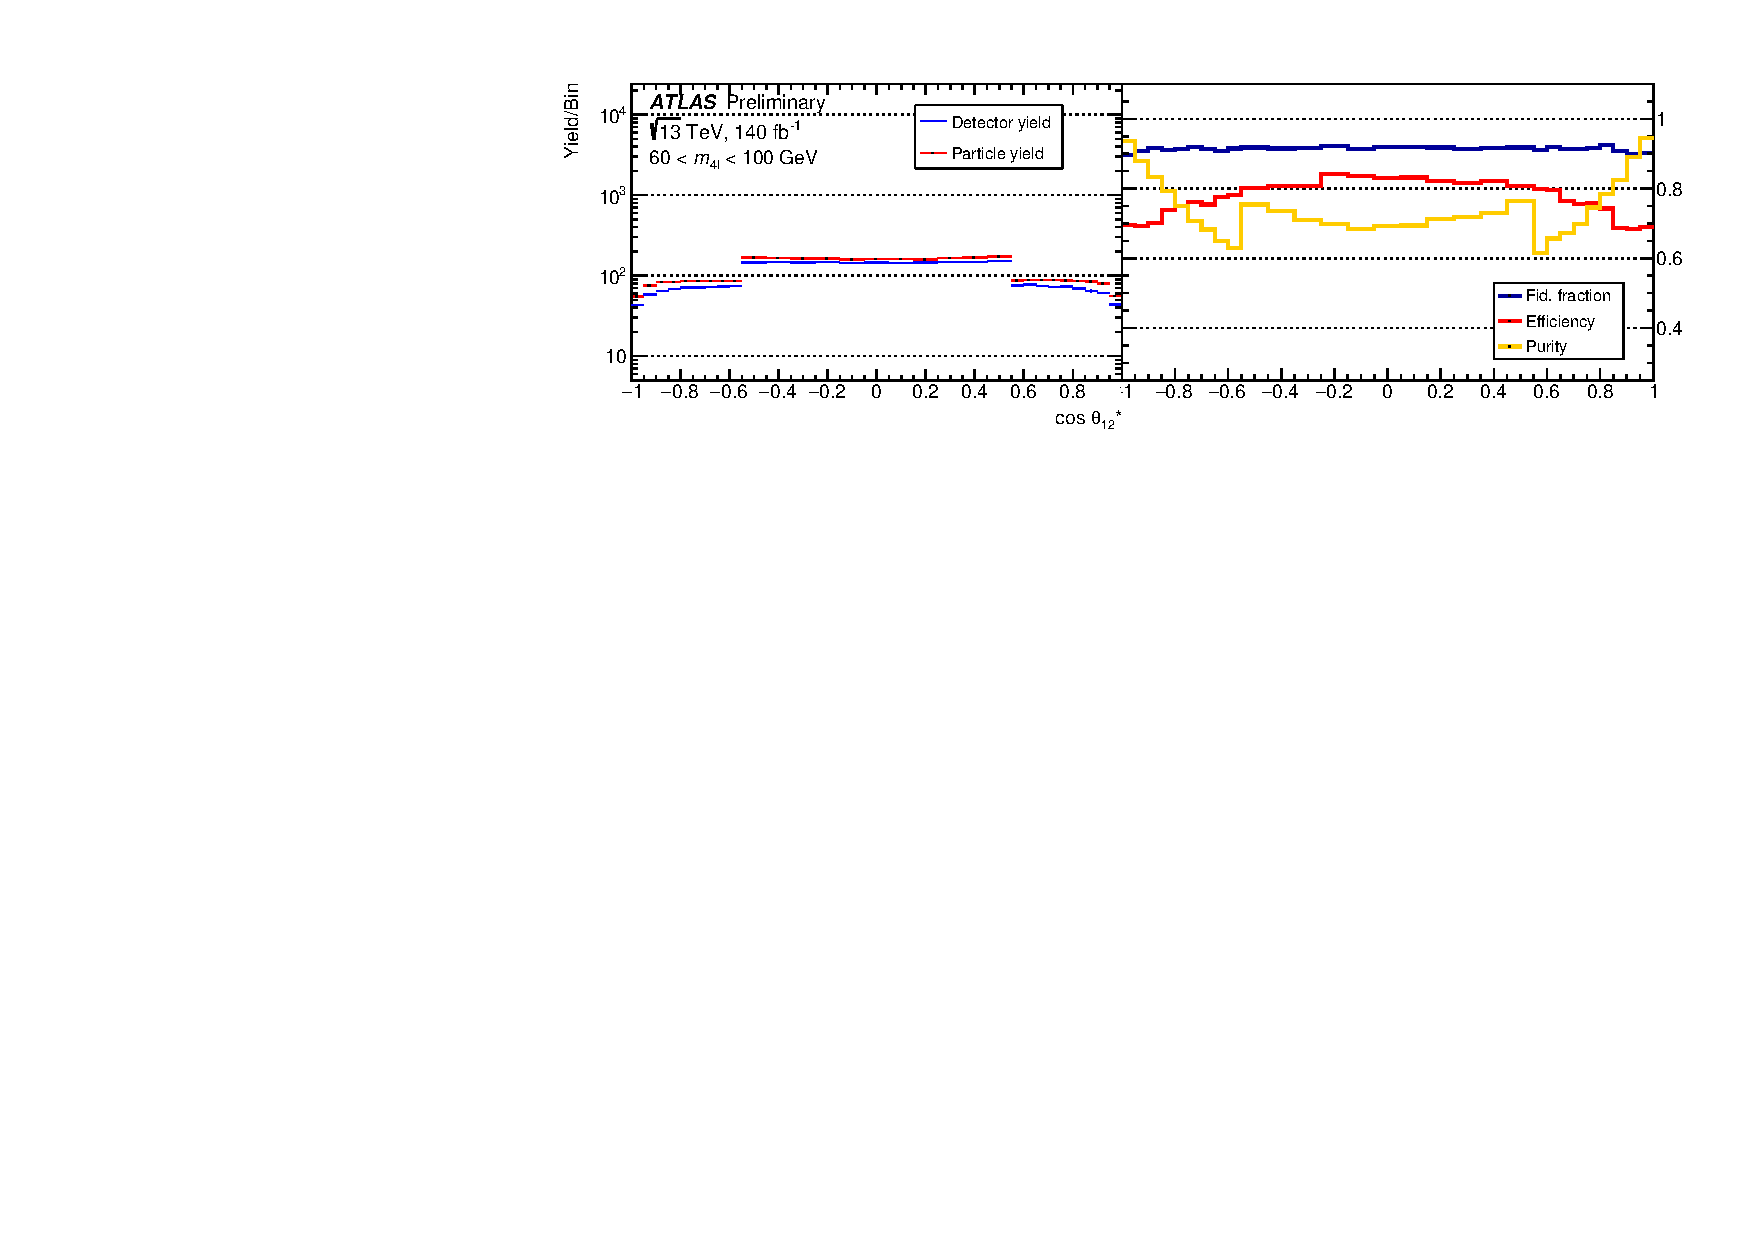
\includegraphics[width = 0.75\textwidth]{figures/UnfoldingStudies/v014_inputs/cosThetaStar1_m4l60-100inputs.pdf}}\\
  \subfigure{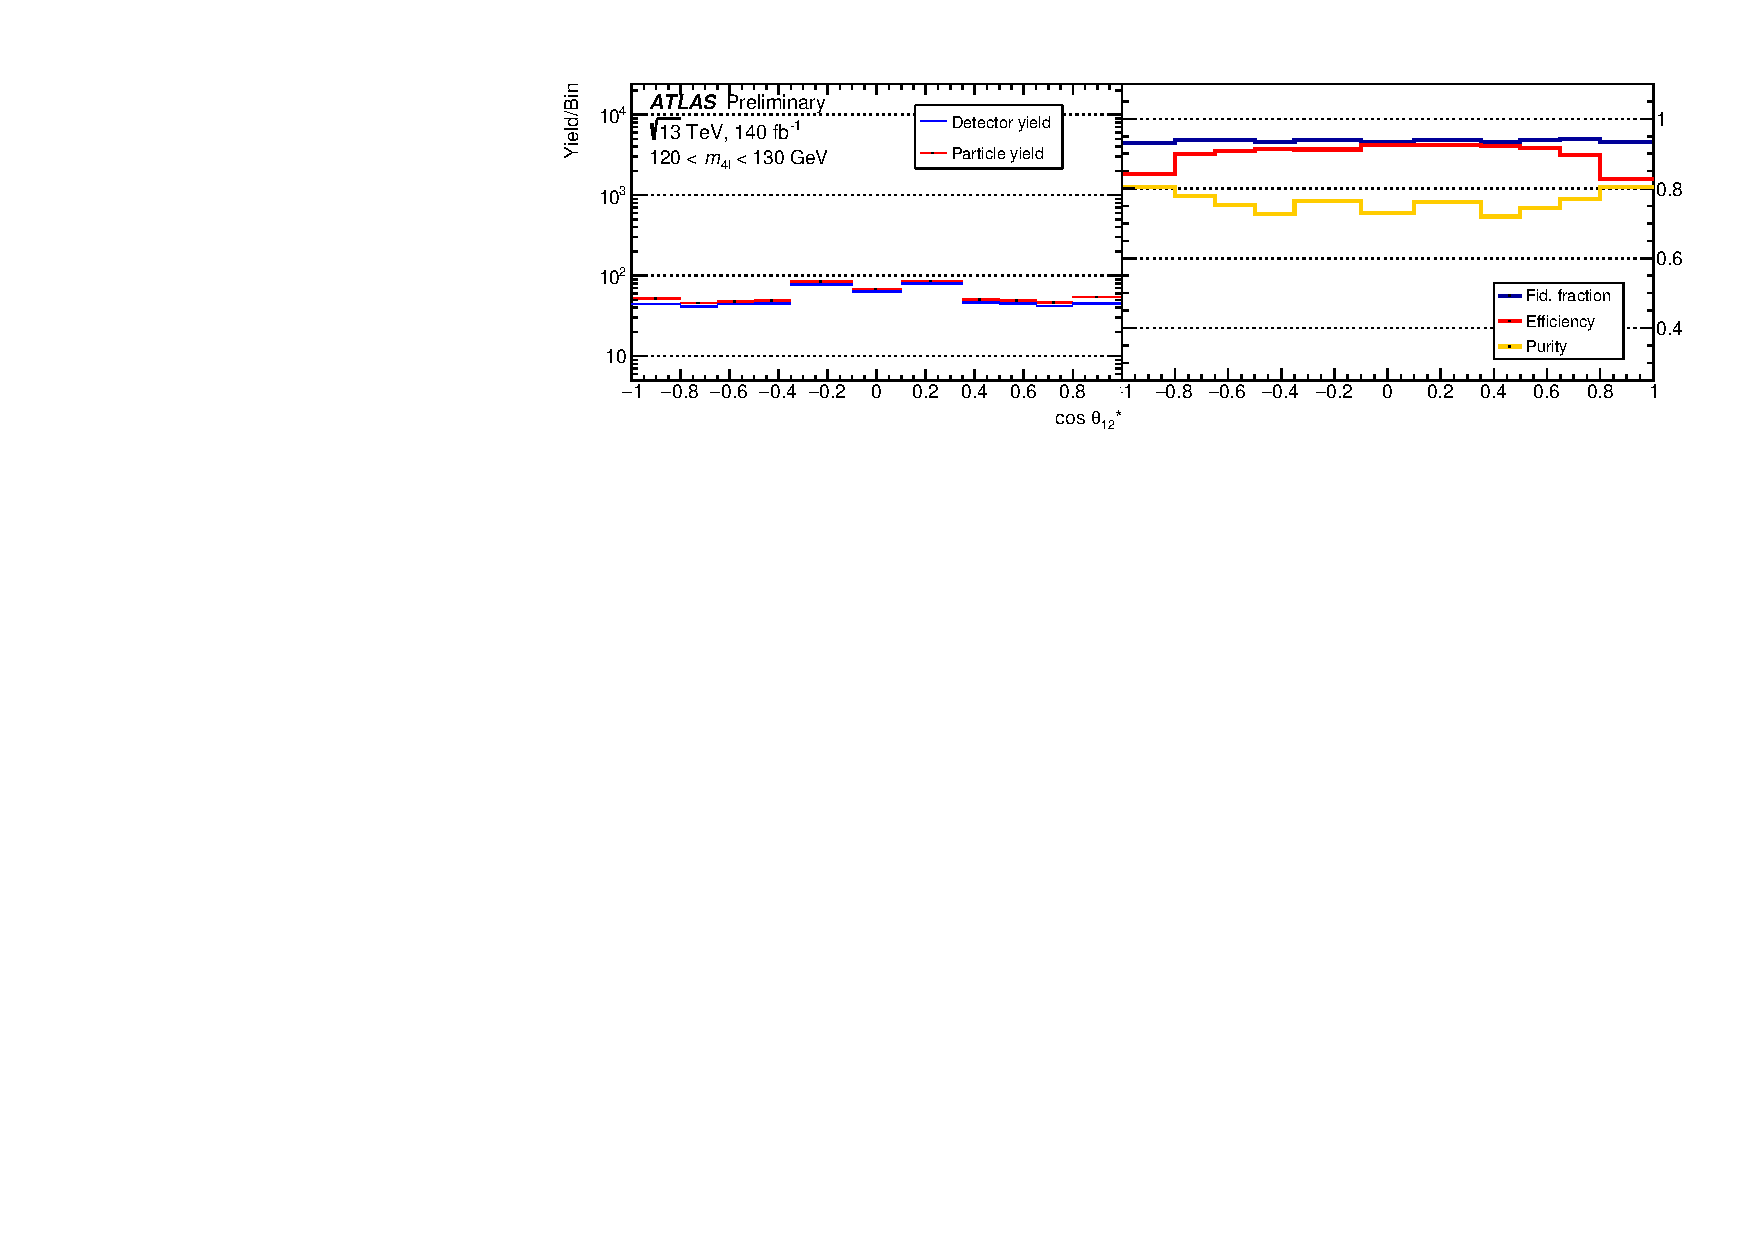
\includegraphics[width = 0.75\textwidth]{figures/UnfoldingStudies/v014_inputs/cosThetaStar1_m4l120-130inputs.pdf}}\\
  \subfigure{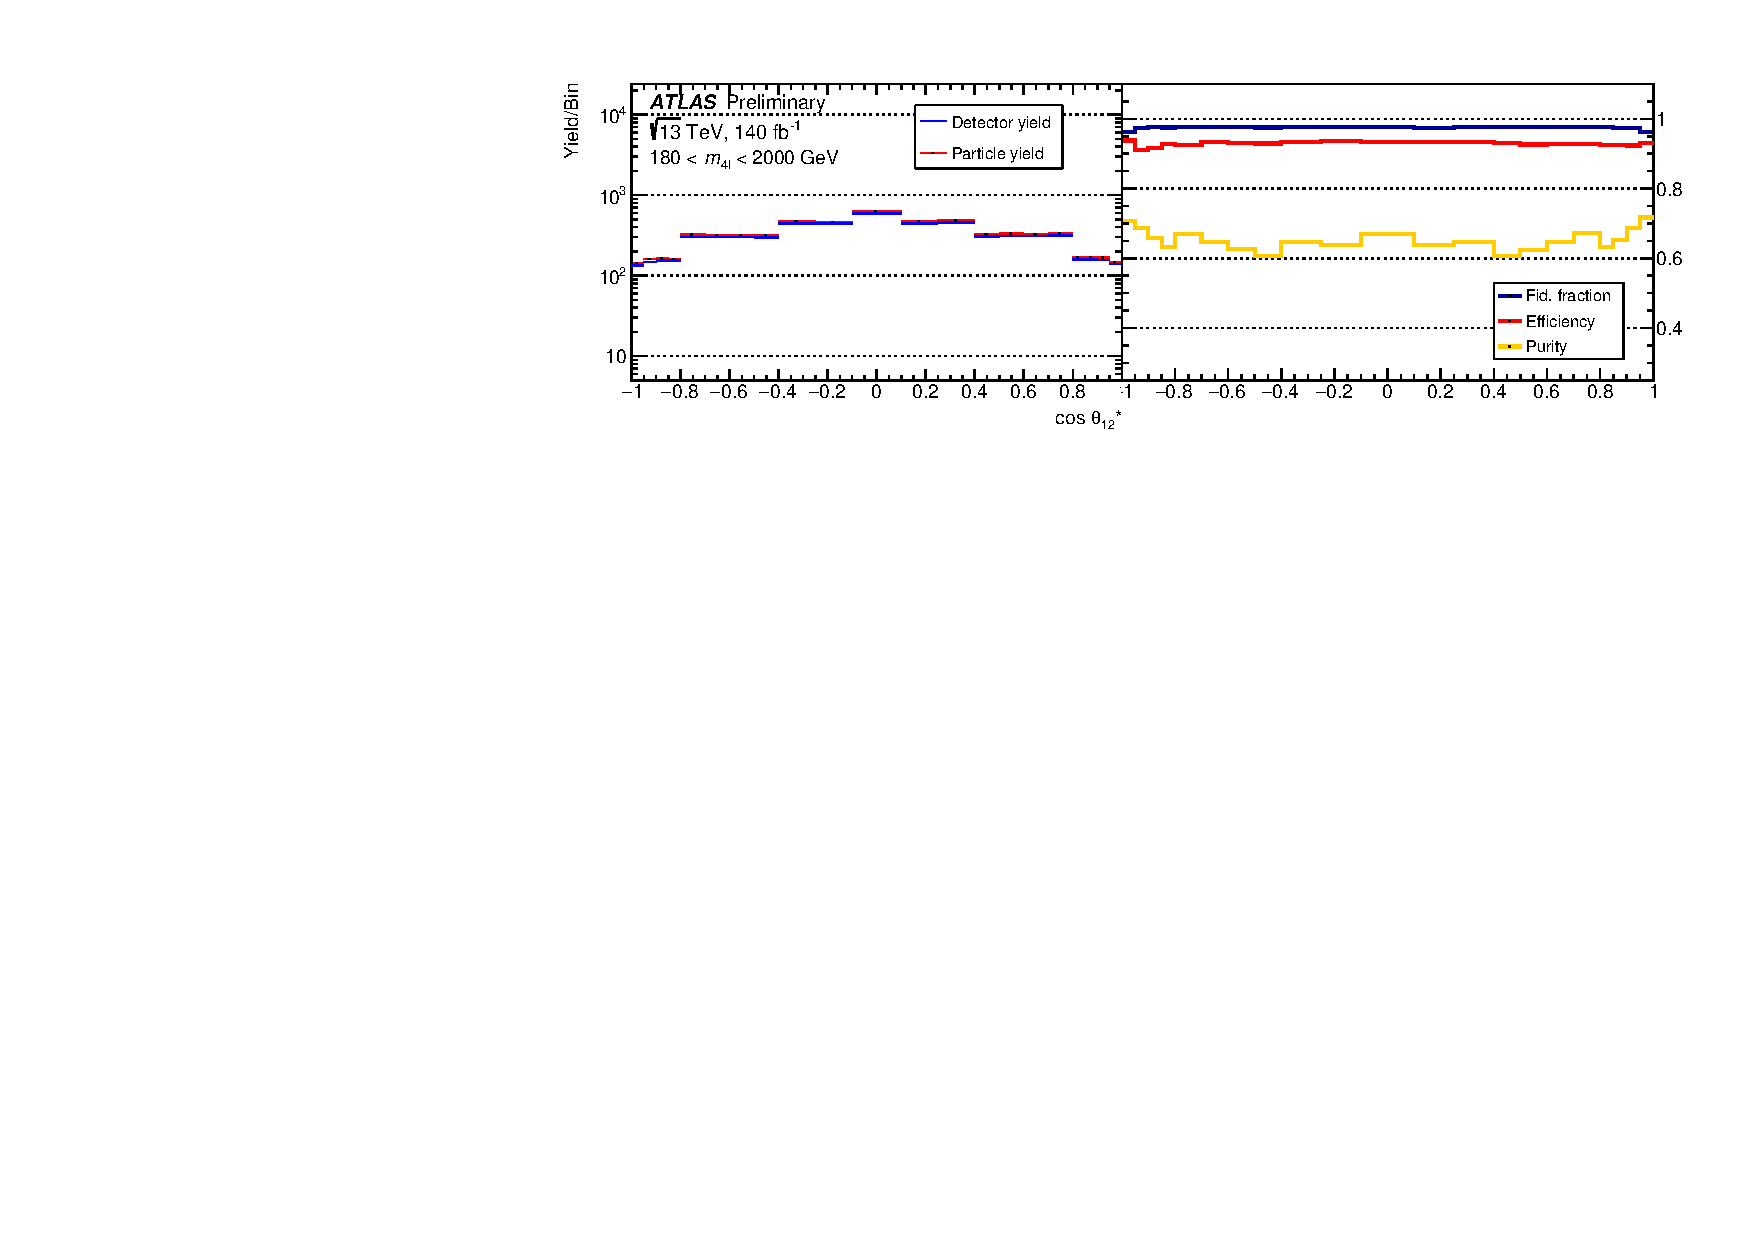
\includegraphics[width = 0.75\textwidth]{figures/UnfoldingStudies/v014_inputs/cosThetaStar1_m4l180-2000inputs.pdf}}\\
  \subfigure{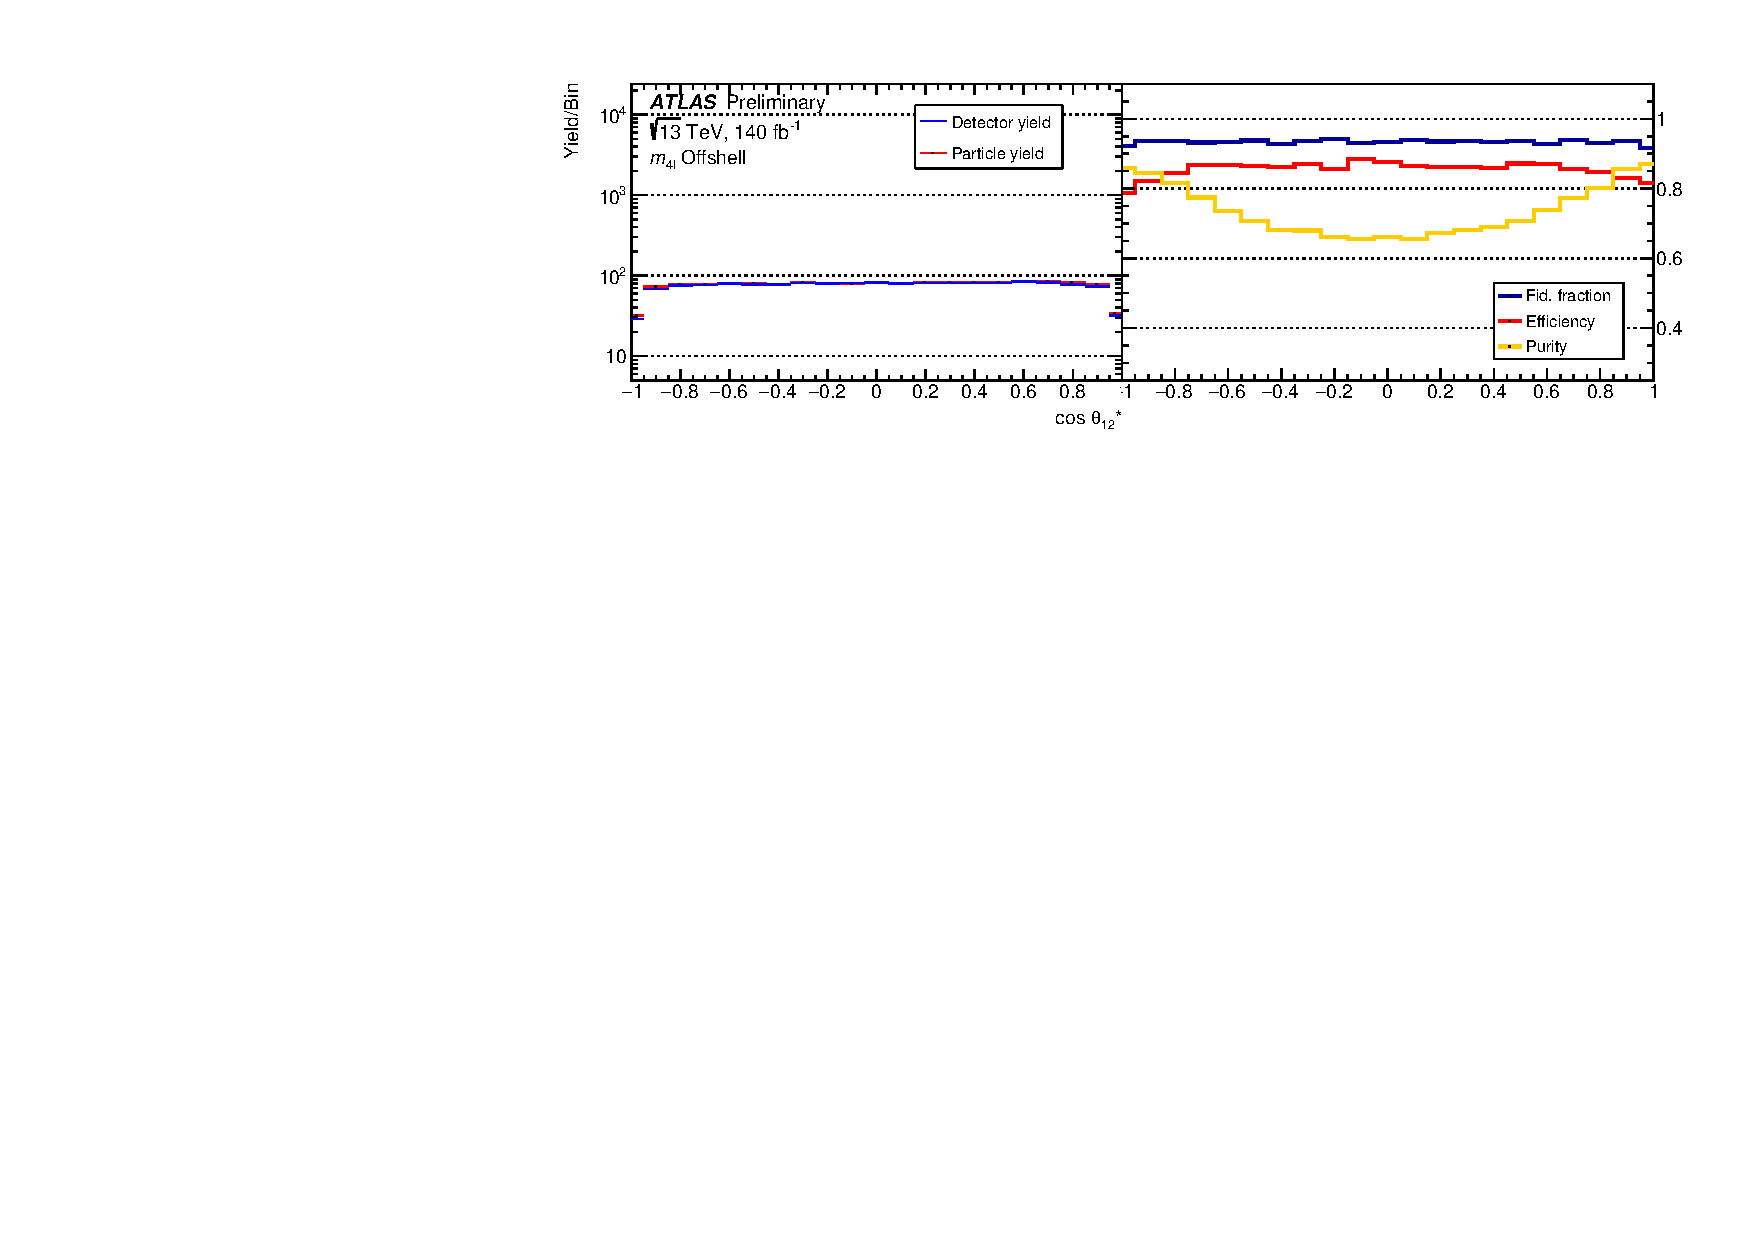
\includegraphics[width = 0.75\textwidth]{figures/UnfoldingStudies/v014_inputs/cosThetaStar1_m4loffshellinputs.pdf}}\\
\caption{In the left-hand panels, the number of predicted events passing the reconstruction- and fiducial- level selections are displayed as the detector yield and particle yield, respectively. The right-hand panel shows the efficiency, fiducial purity and fiducial fraction. All variables are plotted as a function of the \costhetastar bins, in slices of the \mFourL variable which are stacked and labelled with the included \mFourL range.
  \label{fig:costhet1unf}}
 \end{figure}  

\FloatBarrier
\clearpage

\begin{figure}[htb]
  \centering 
  \subfigure{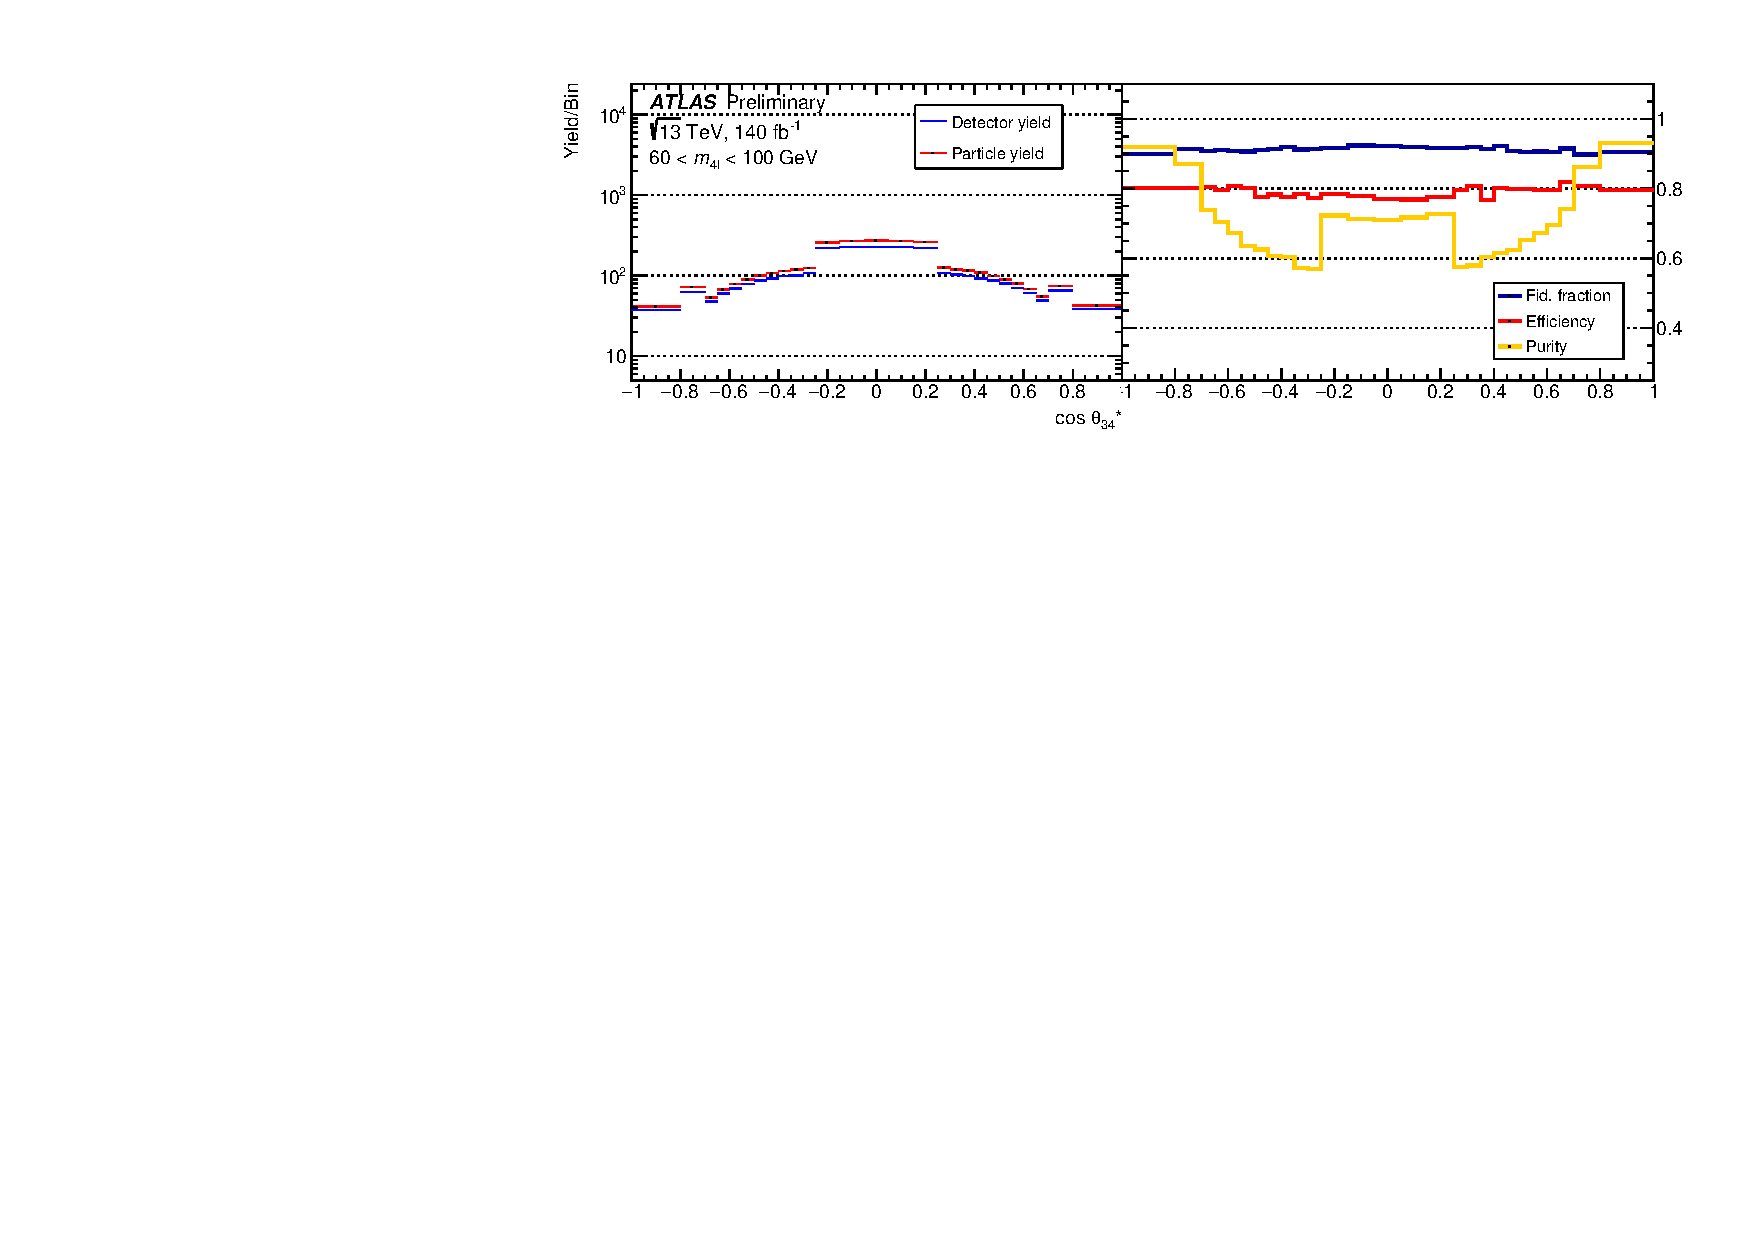
\includegraphics[width = 0.75\textwidth]{figures/UnfoldingStudies/v014_inputs/cosThetaStar3_m4l60-100inputs.pdf}}\\
  \subfigure{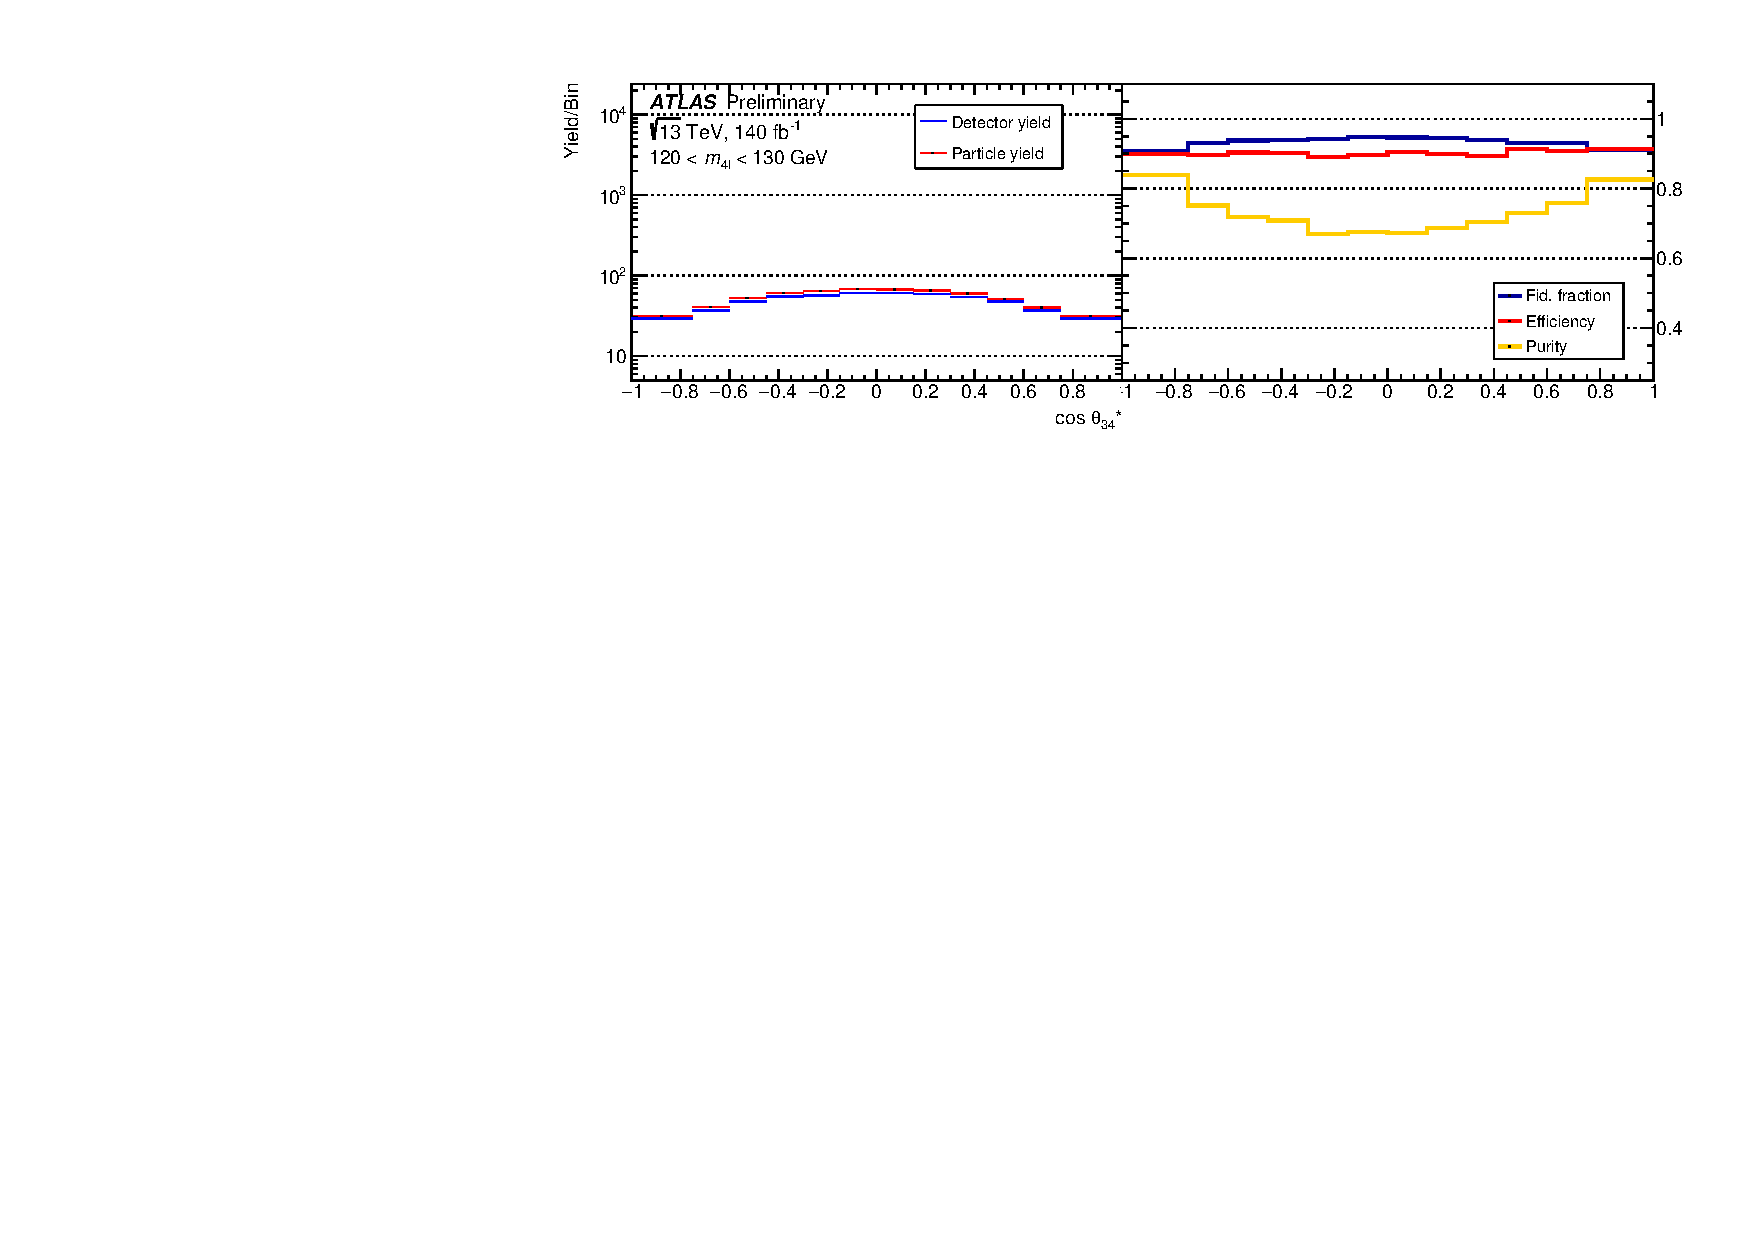
\includegraphics[width = 0.75\textwidth]{figures/UnfoldingStudies/v014_inputs/cosThetaStar3_m4l120-130inputs.pdf}}\\
  \subfigure{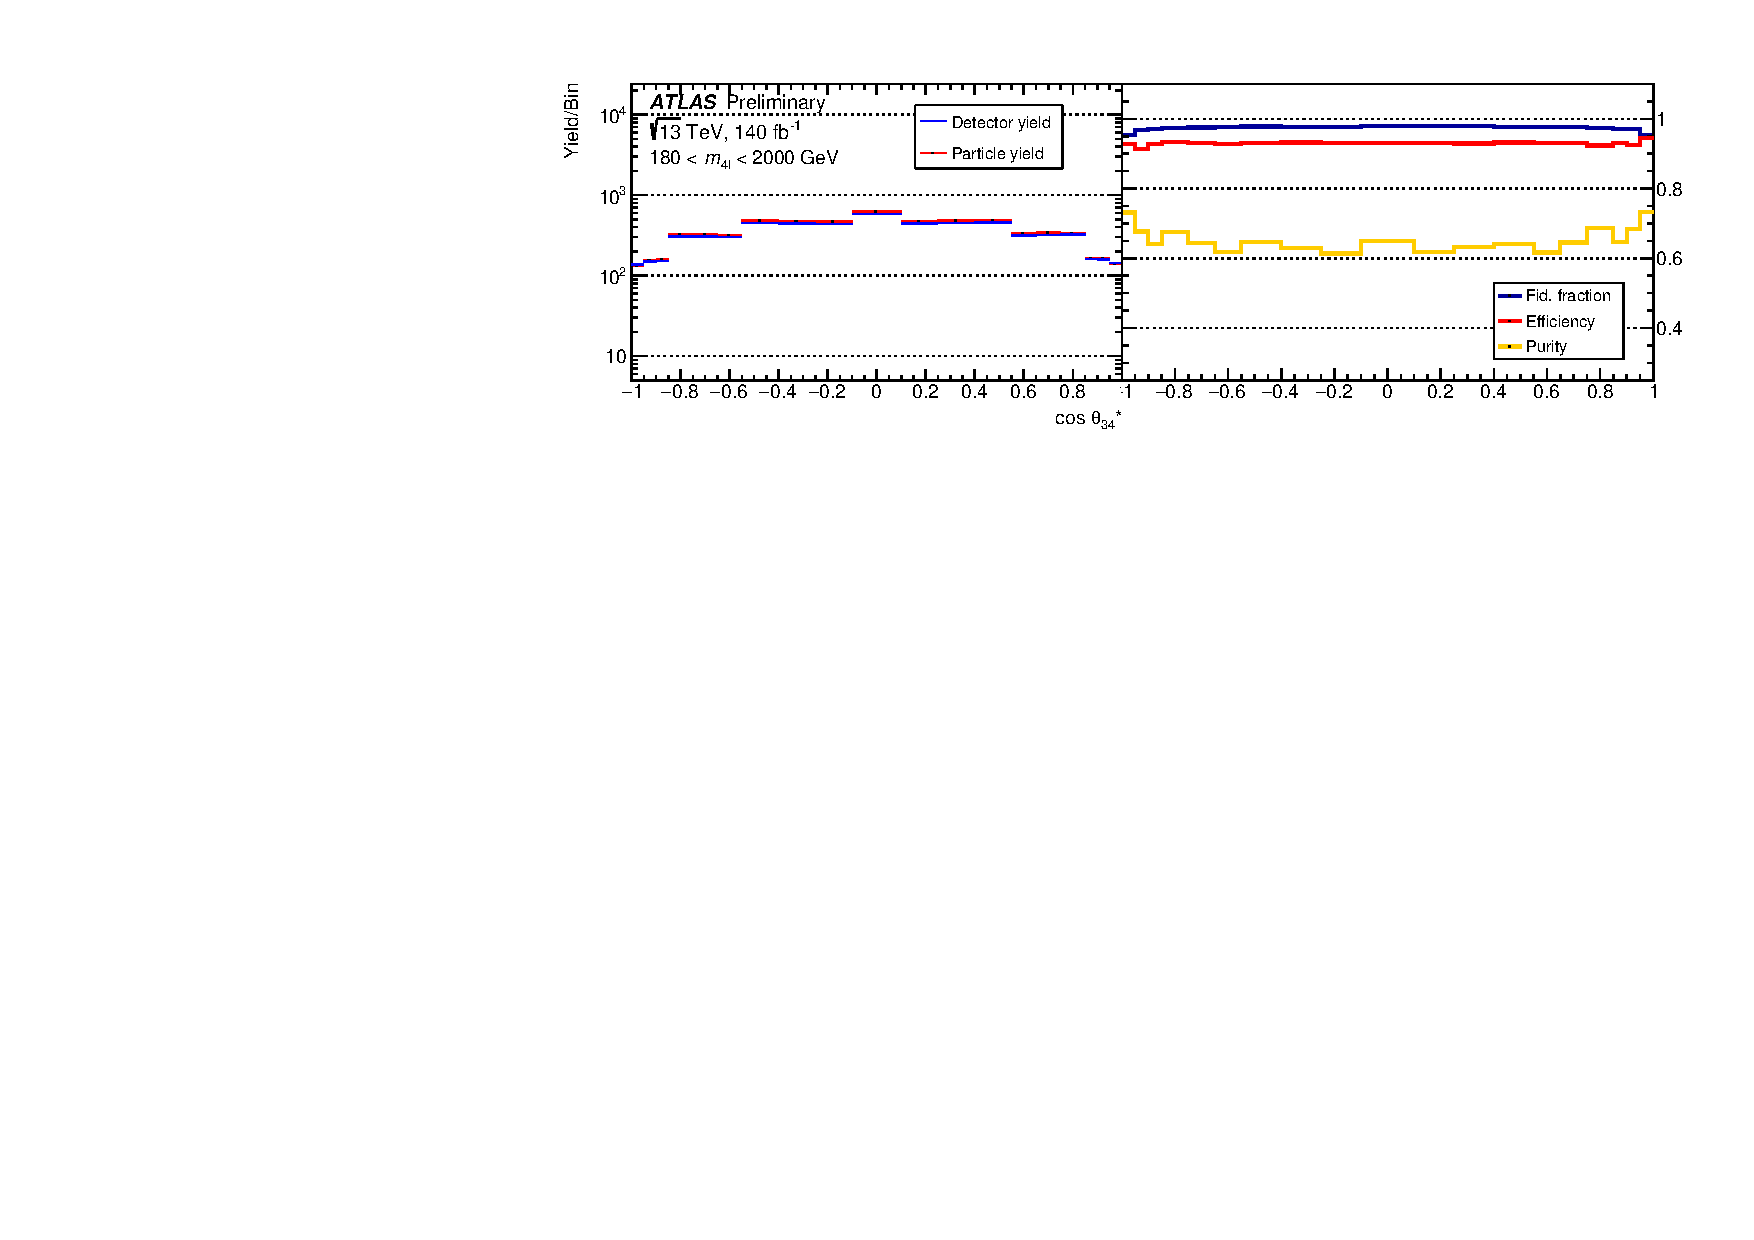
\includegraphics[width = 0.75\textwidth]{figures/UnfoldingStudies/v014_inputs/cosThetaStar3_m4l180-2000inputs.pdf}}\\
  \subfigure{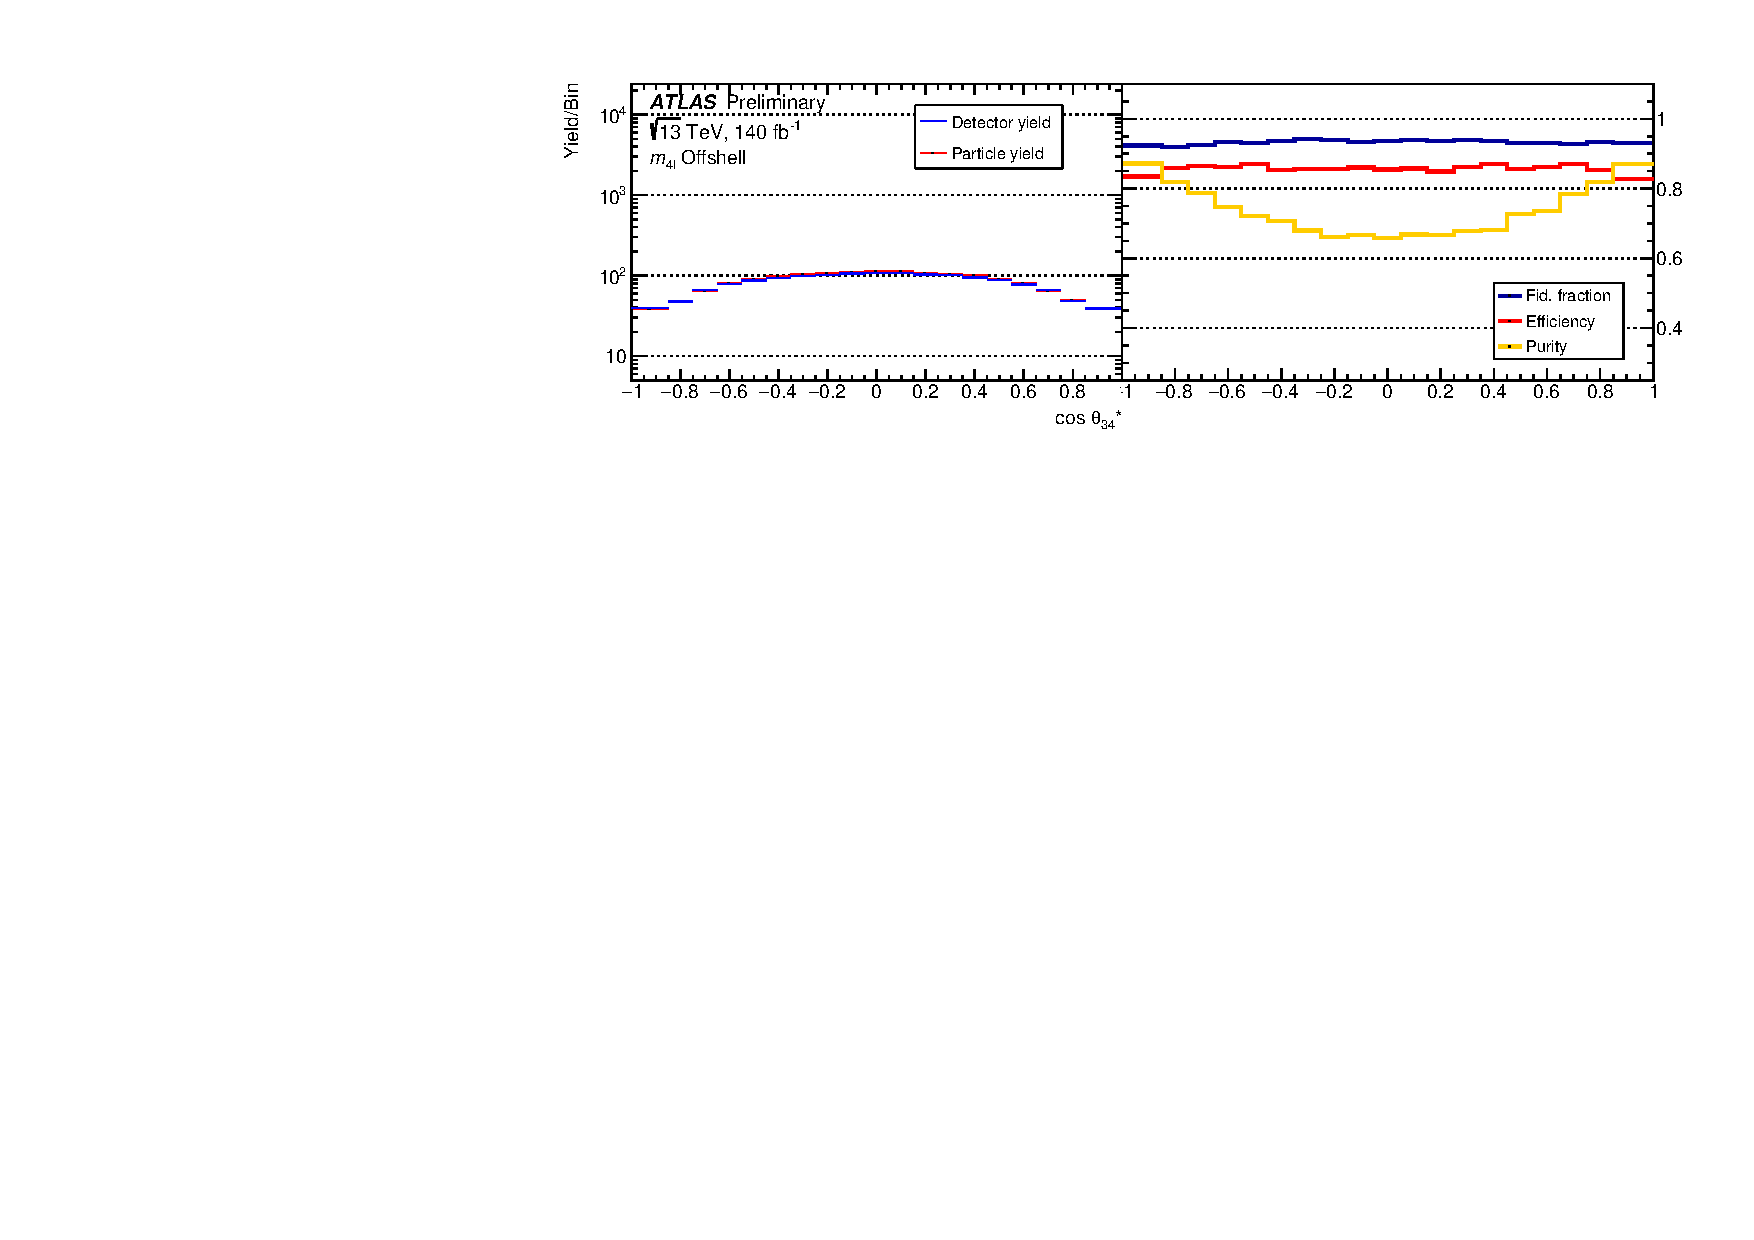
\includegraphics[width = 0.75\textwidth]{figures/UnfoldingStudies/v014_inputs/cosThetaStar3_m4loffshellinputs.pdf}}\\
\caption{In the left-hand panels, the number of predicted events passing the reconstruction- and fiducial- level selections are displayed as the detector yield and particle yield, respectively. The right-hand panel shows the efficiency, fiducial purity and fiducial fraction. All variables are plotted as a function of the \costhetastar bins, in slices of the \mFourL variable which are stacked and labelled with the included \mFourL range.
  \label{fig:costhet2unf}}
 \end{figure}  


\FloatBarrier
\clearpage

\begin{figure}[htb]
  \centering 
  \subfigure{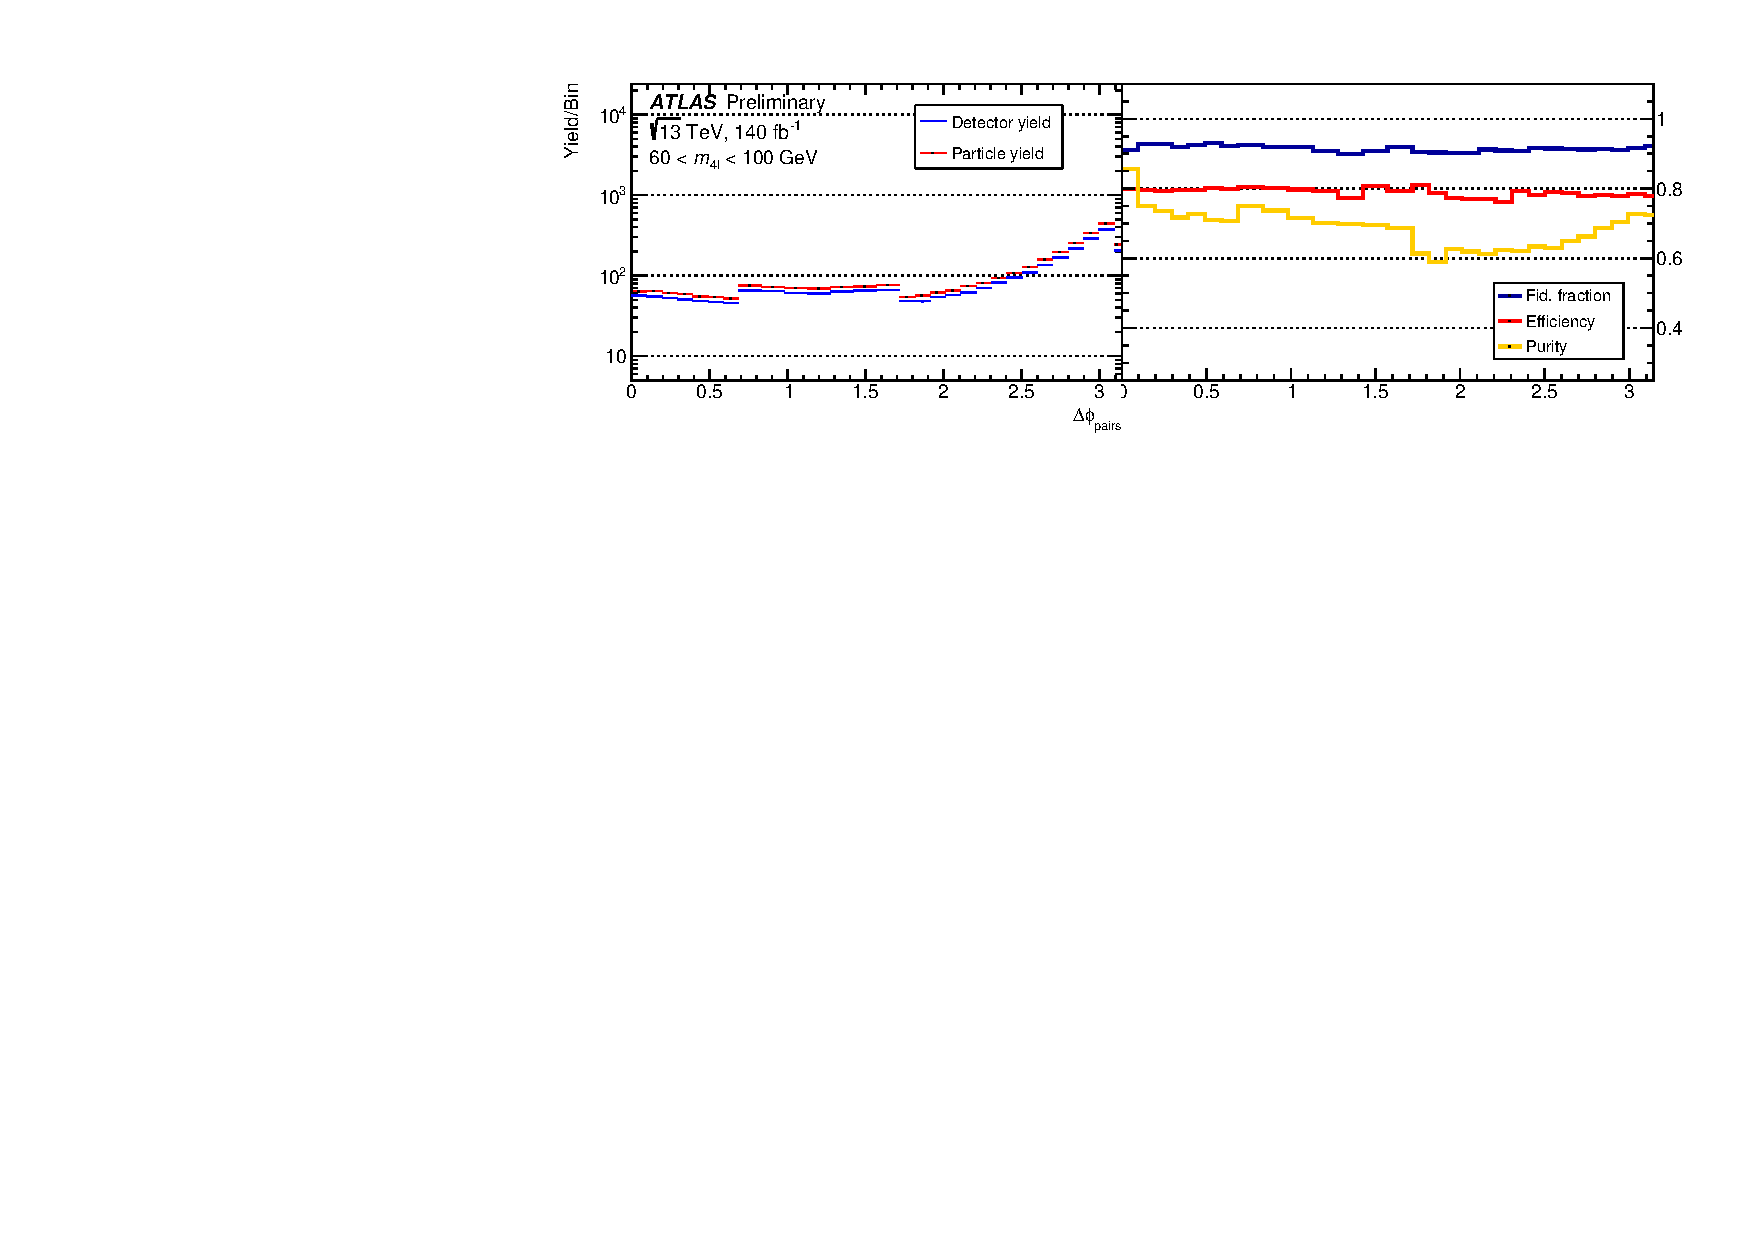
\includegraphics[width = 0.75\textwidth]{figures/UnfoldingStudies/v014_inputs/deltaPhiPairs_m4l60-100inputs.pdf}}\\
  \subfigure{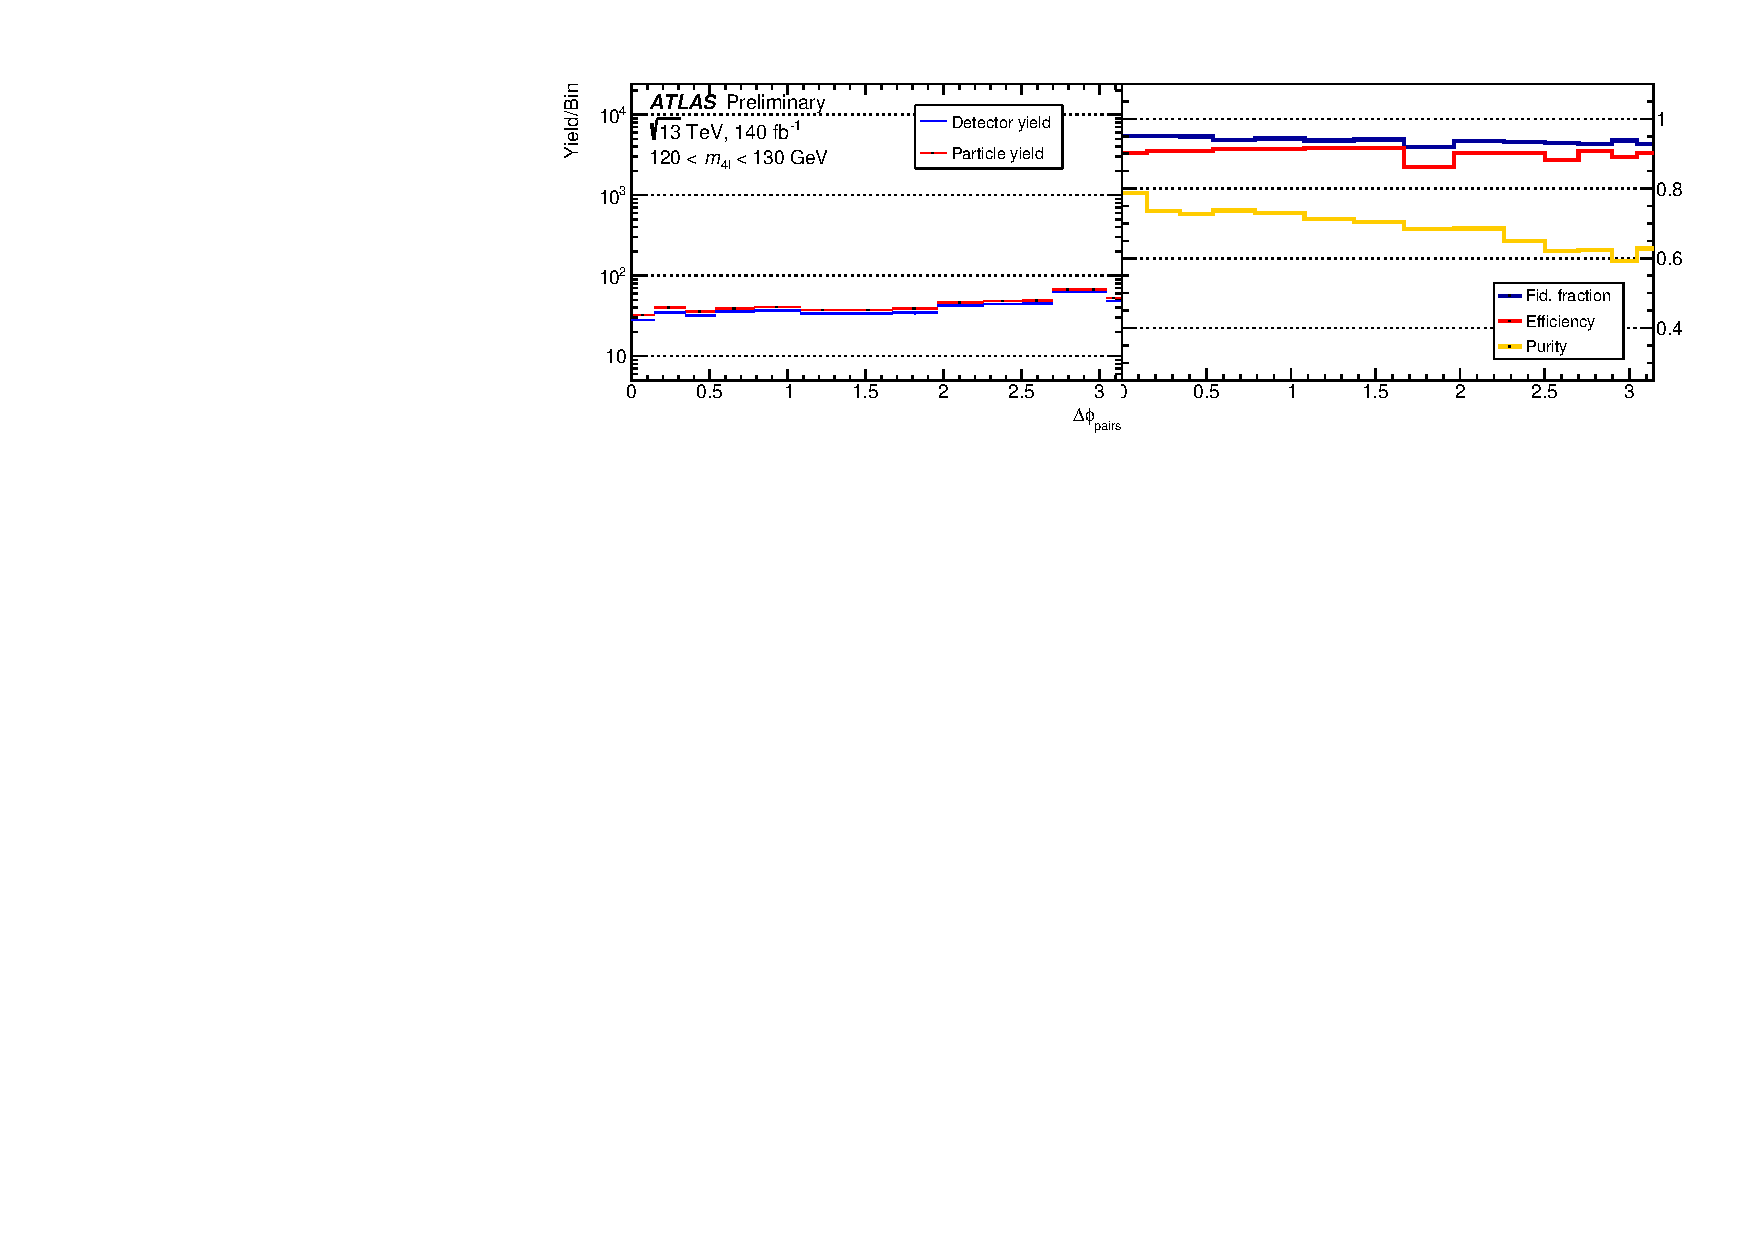
\includegraphics[width = 0.75\textwidth]{figures/UnfoldingStudies/v014_inputs/deltaPhiPairs_m4l120-130inputs.pdf}}\\
  \subfigure{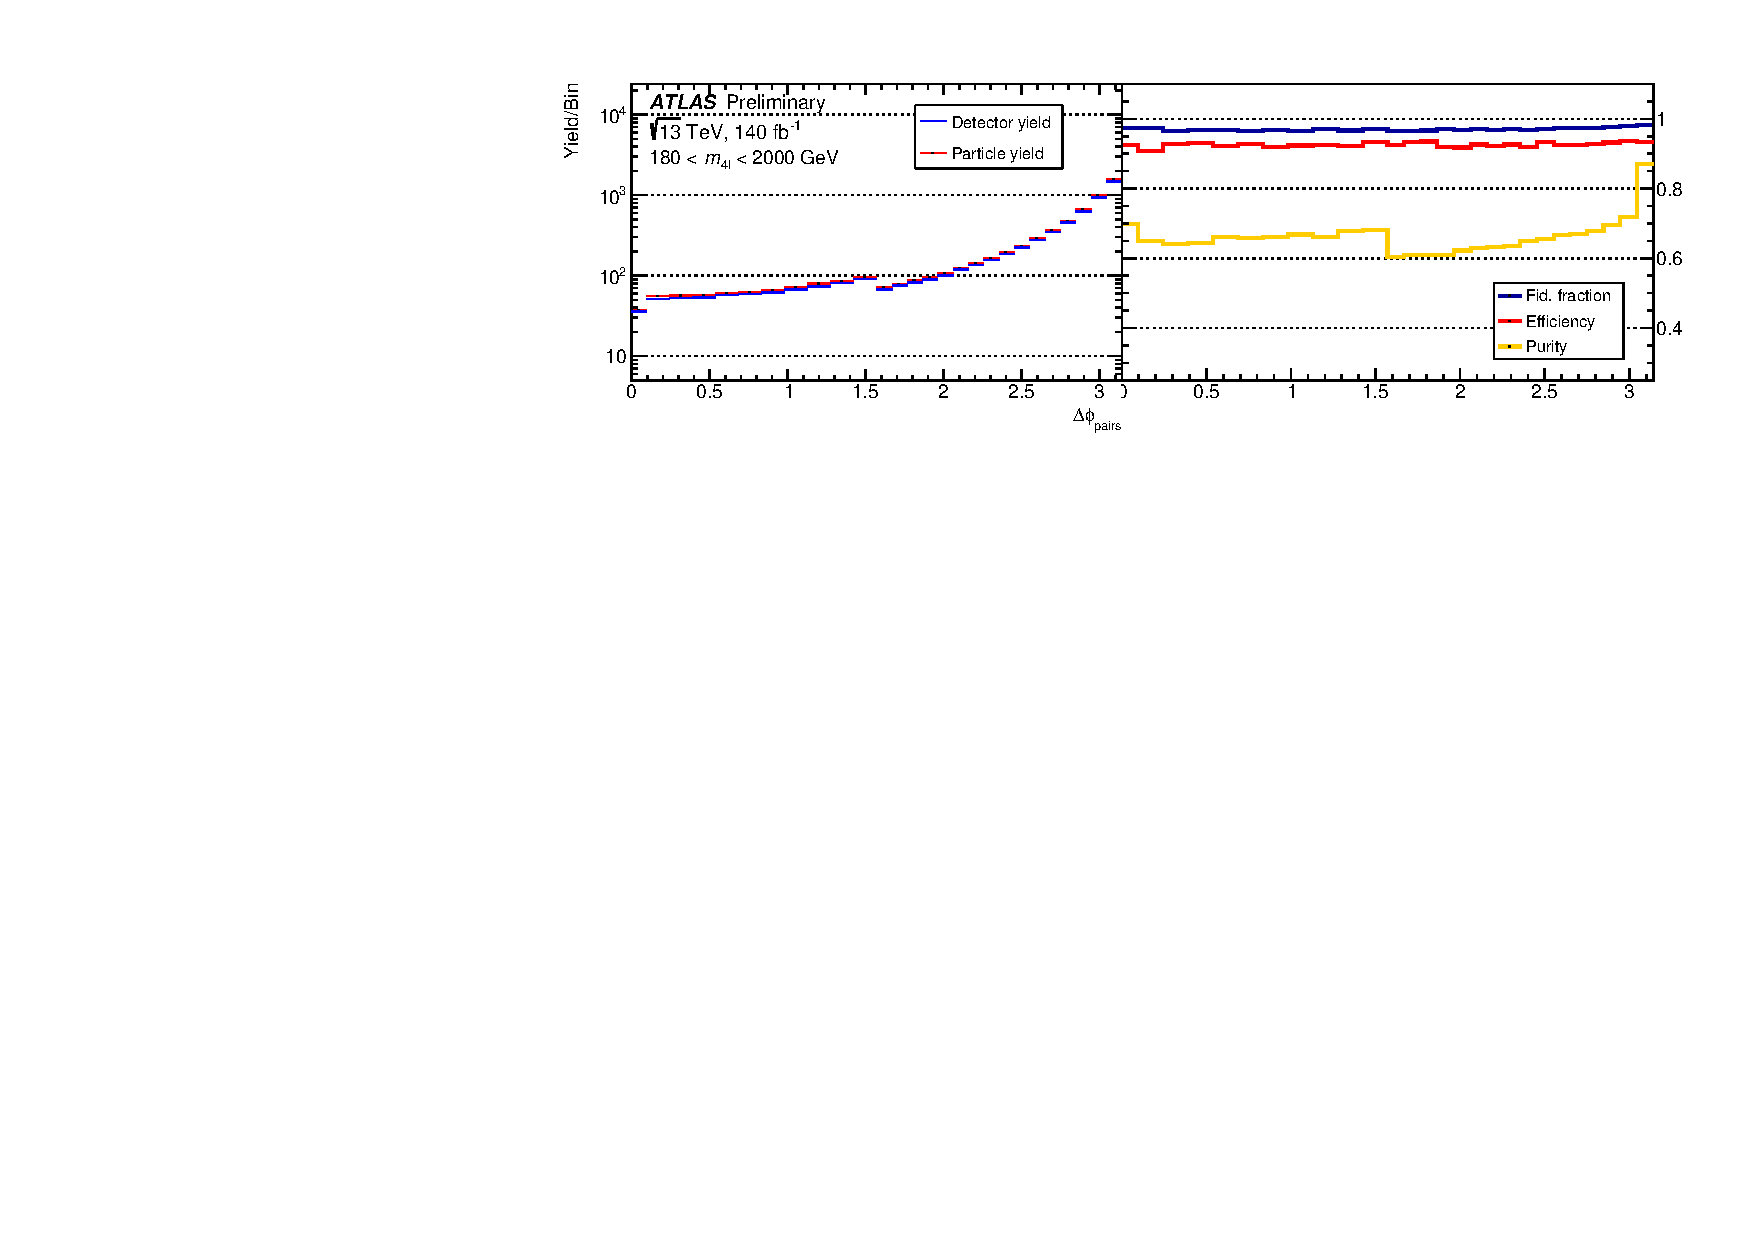
\includegraphics[width = 0.75\textwidth]{figures/UnfoldingStudies/v014_inputs/deltaPhiPairs_m4l180-2000inputs.pdf}}\\
  \subfigure{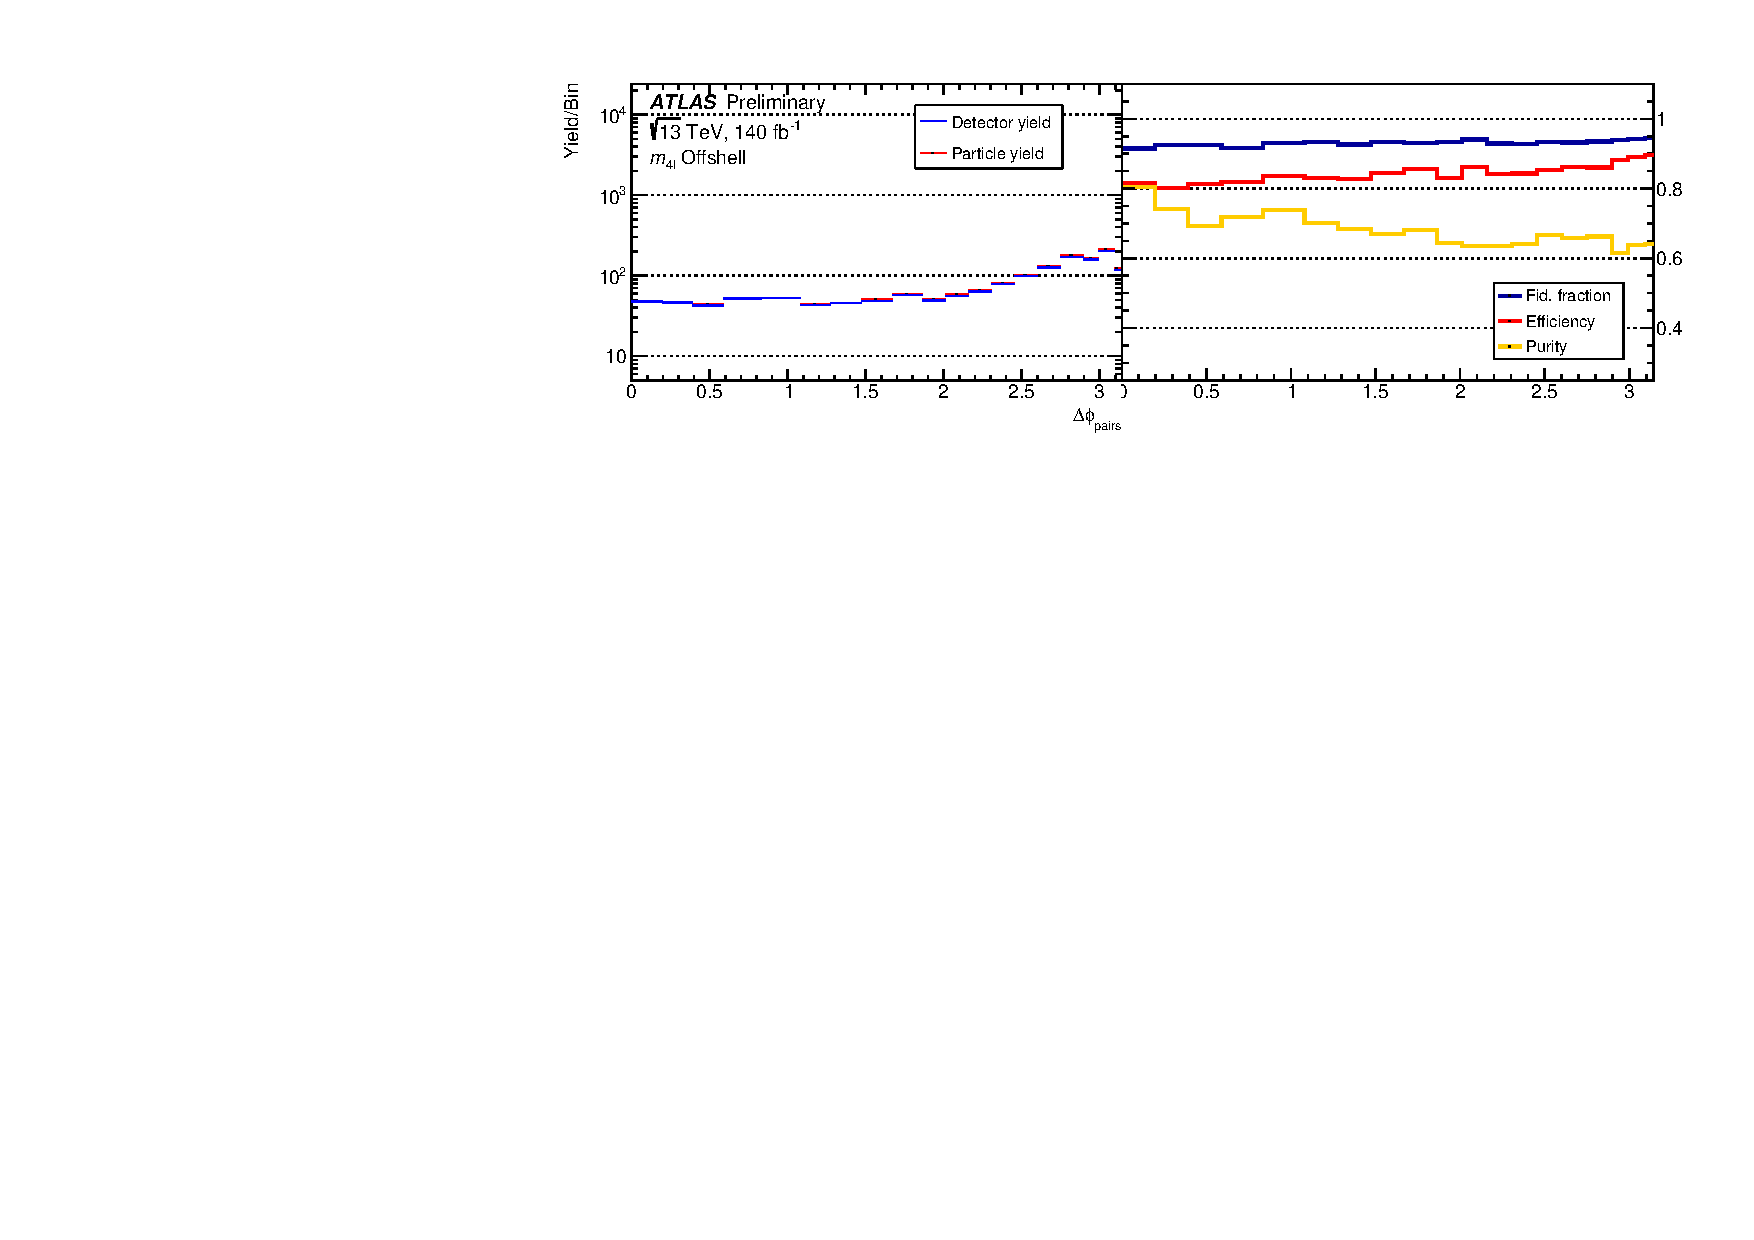
\includegraphics[width = 0.75\textwidth]{figures/UnfoldingStudies/v014_inputs/deltaPhiPairs_m4loffshellinputs.pdf}}\\
\caption{In the left-hand panels, the number of predicted events passing the reconstruction- and fiducial- level selections are displayed as the detector yield and particle yield, respectively. The right-hand panel shows the efficiency, fiducial purity and fiducial fraction. All variables are plotted as a function of the \dPhiPairs bins, in slices of the \mFourL variable which are stacked and labelled with the included \mFourL range.
  \label{fig:dphipunf}}
 \end{figure}  


\FloatBarrier
\clearpage

\begin{figure}[htb]
  \centering 
  \subfigure{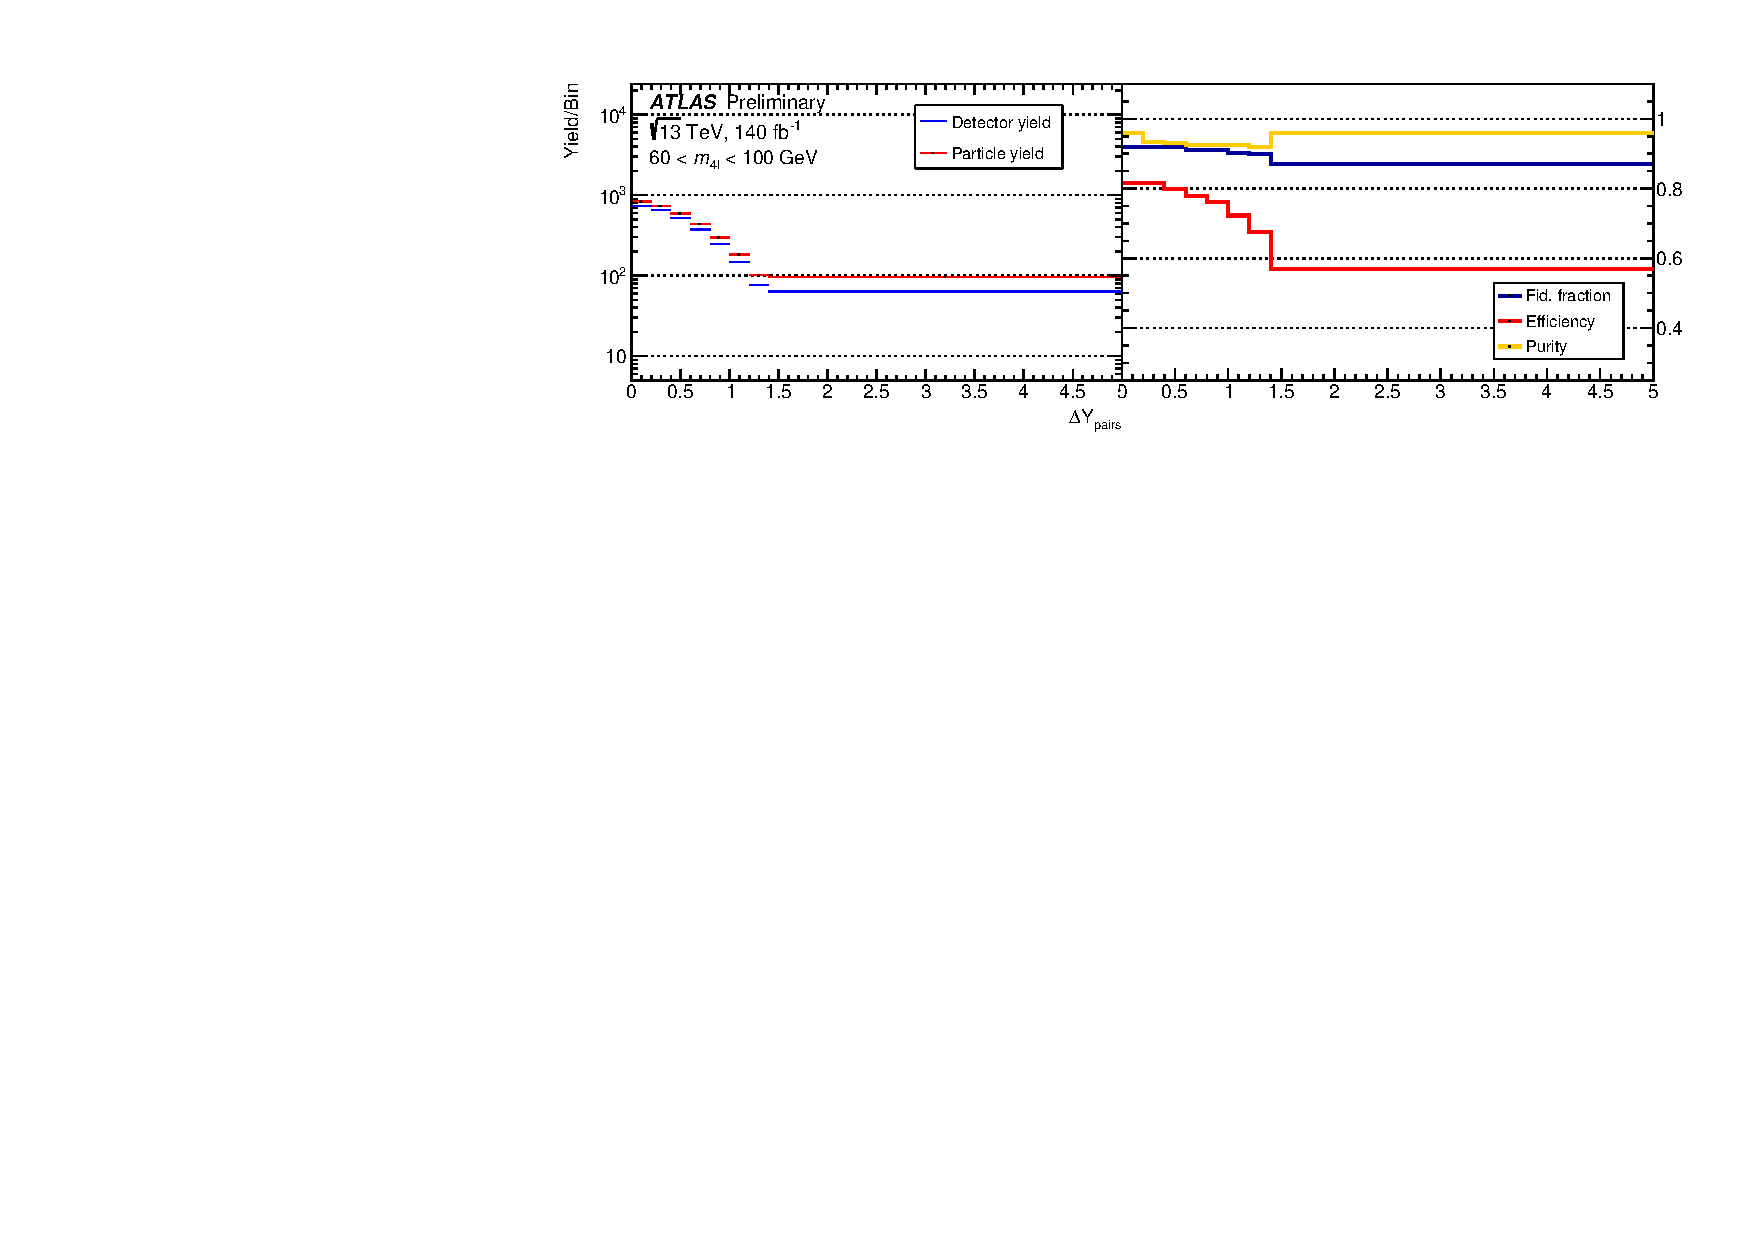
\includegraphics[width = 0.75\textwidth]{figures/UnfoldingStudies/v014_inputs/deltaYPairs_m4l60-100inputs.pdf}}\\
  \subfigure{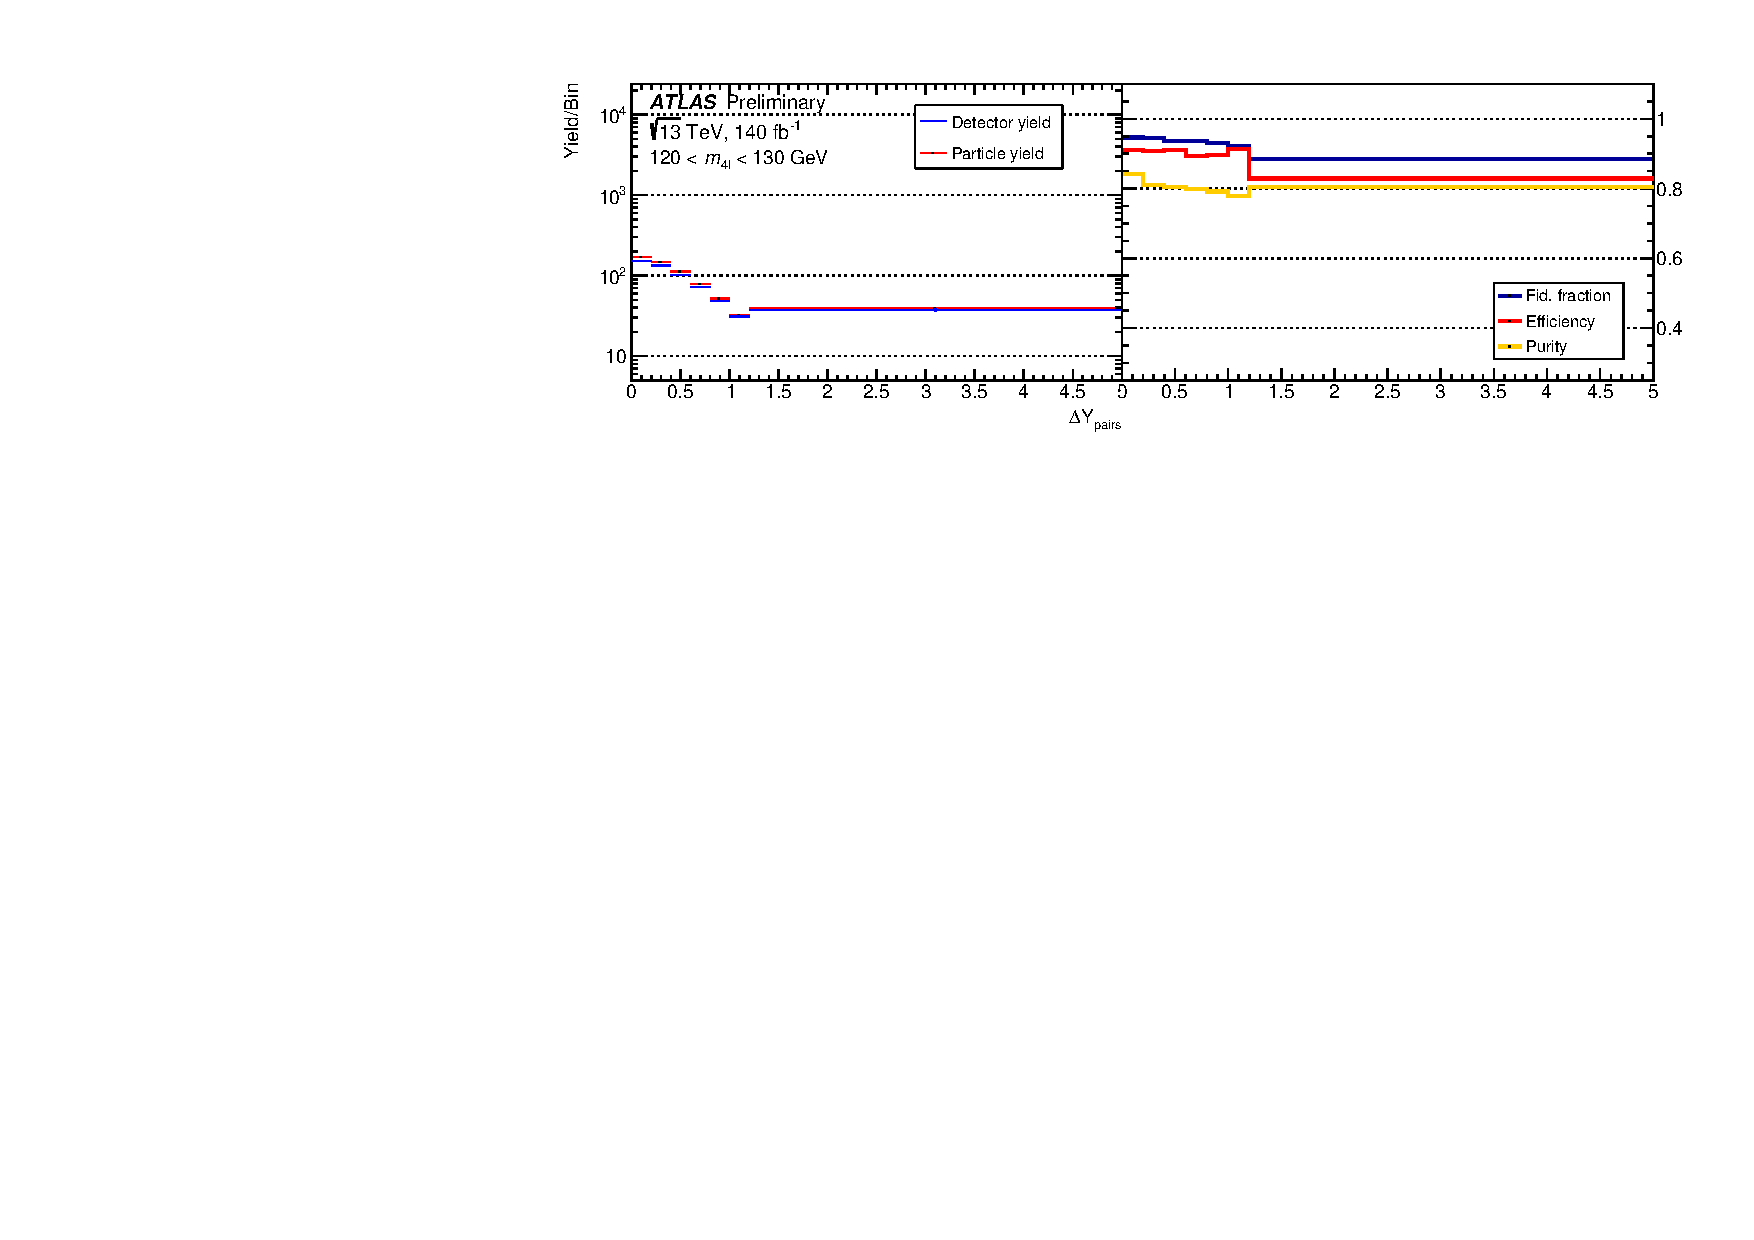
\includegraphics[width = 0.75\textwidth]{figures/UnfoldingStudies/v014_inputs/deltaYPairs_m4l120-130inputs.pdf}}\\
  \subfigure{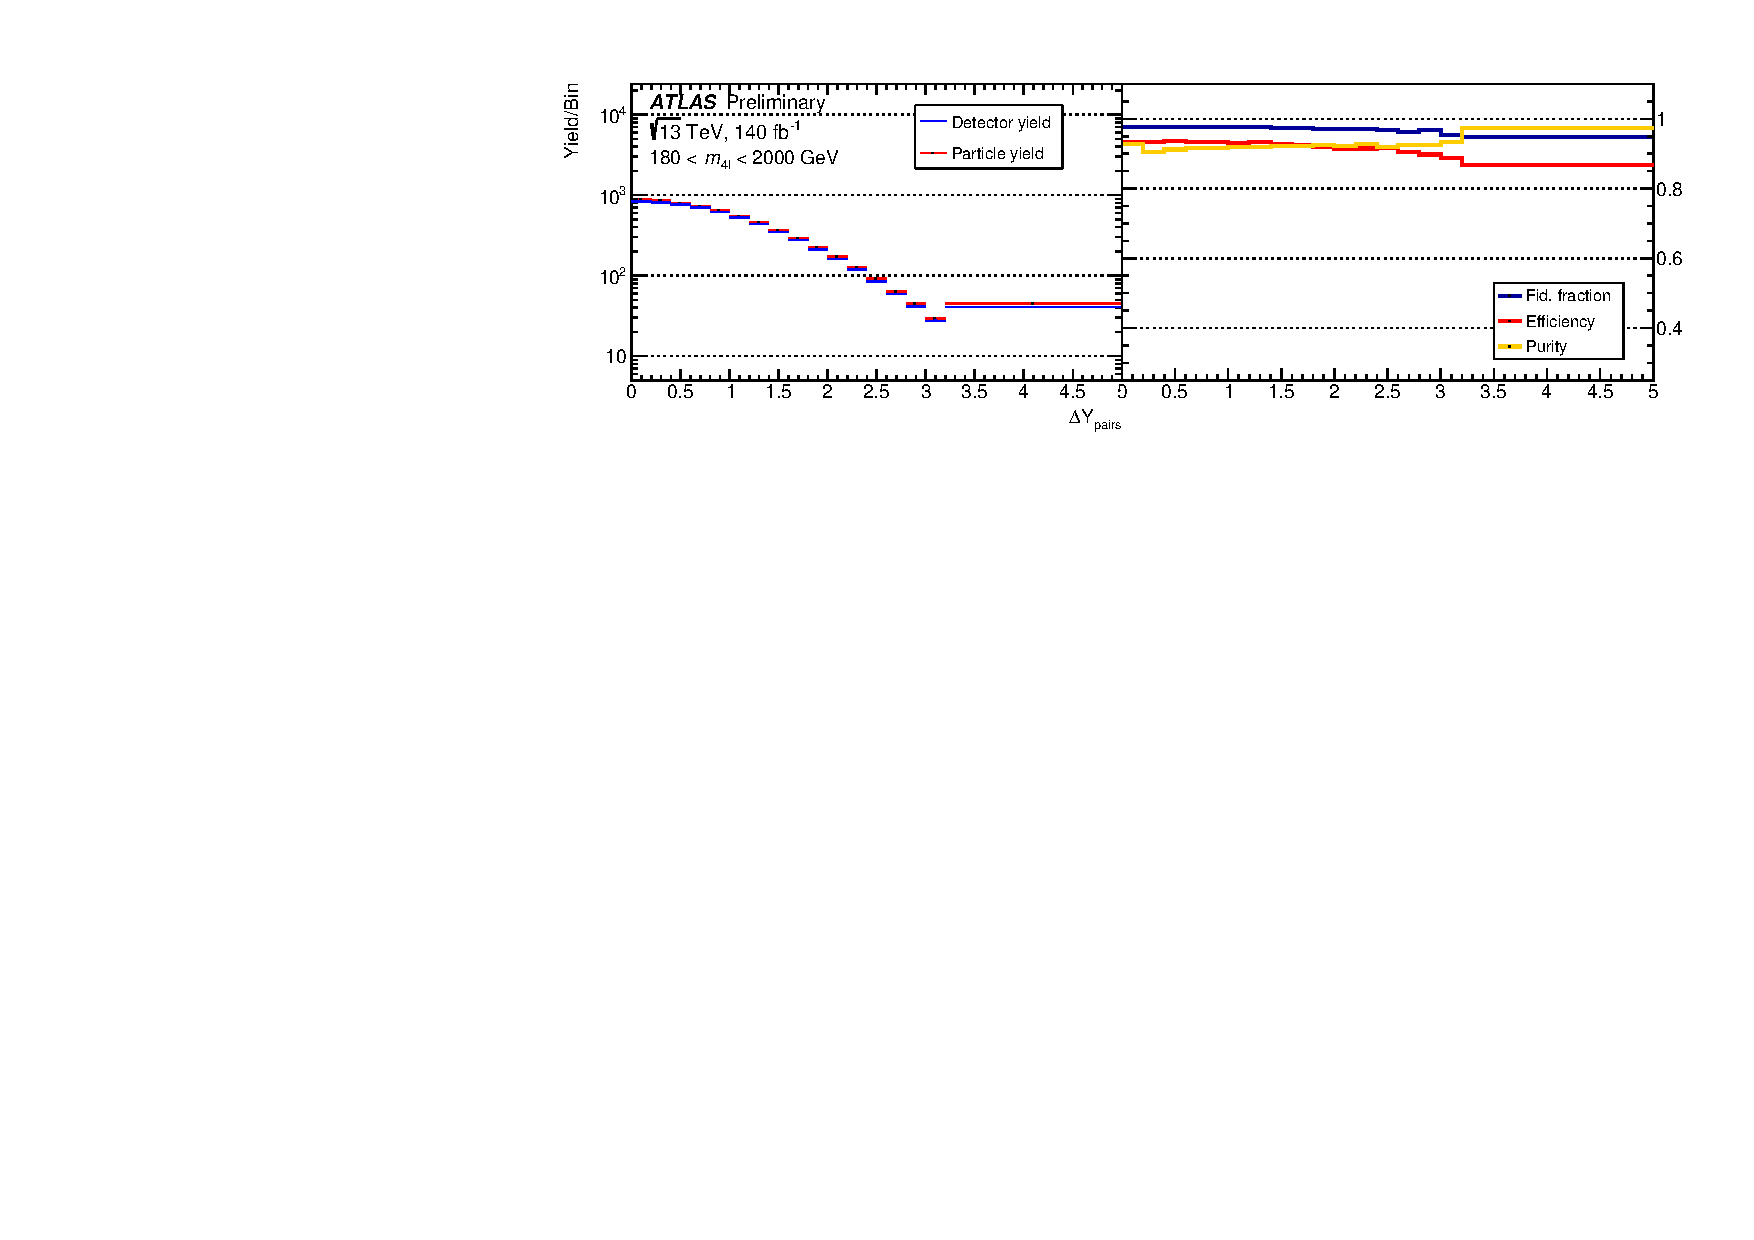
\includegraphics[width = 0.75\textwidth]{figures/UnfoldingStudies/v014_inputs/deltaYPairs_m4l180-2000inputs.pdf}}\\
  \subfigure{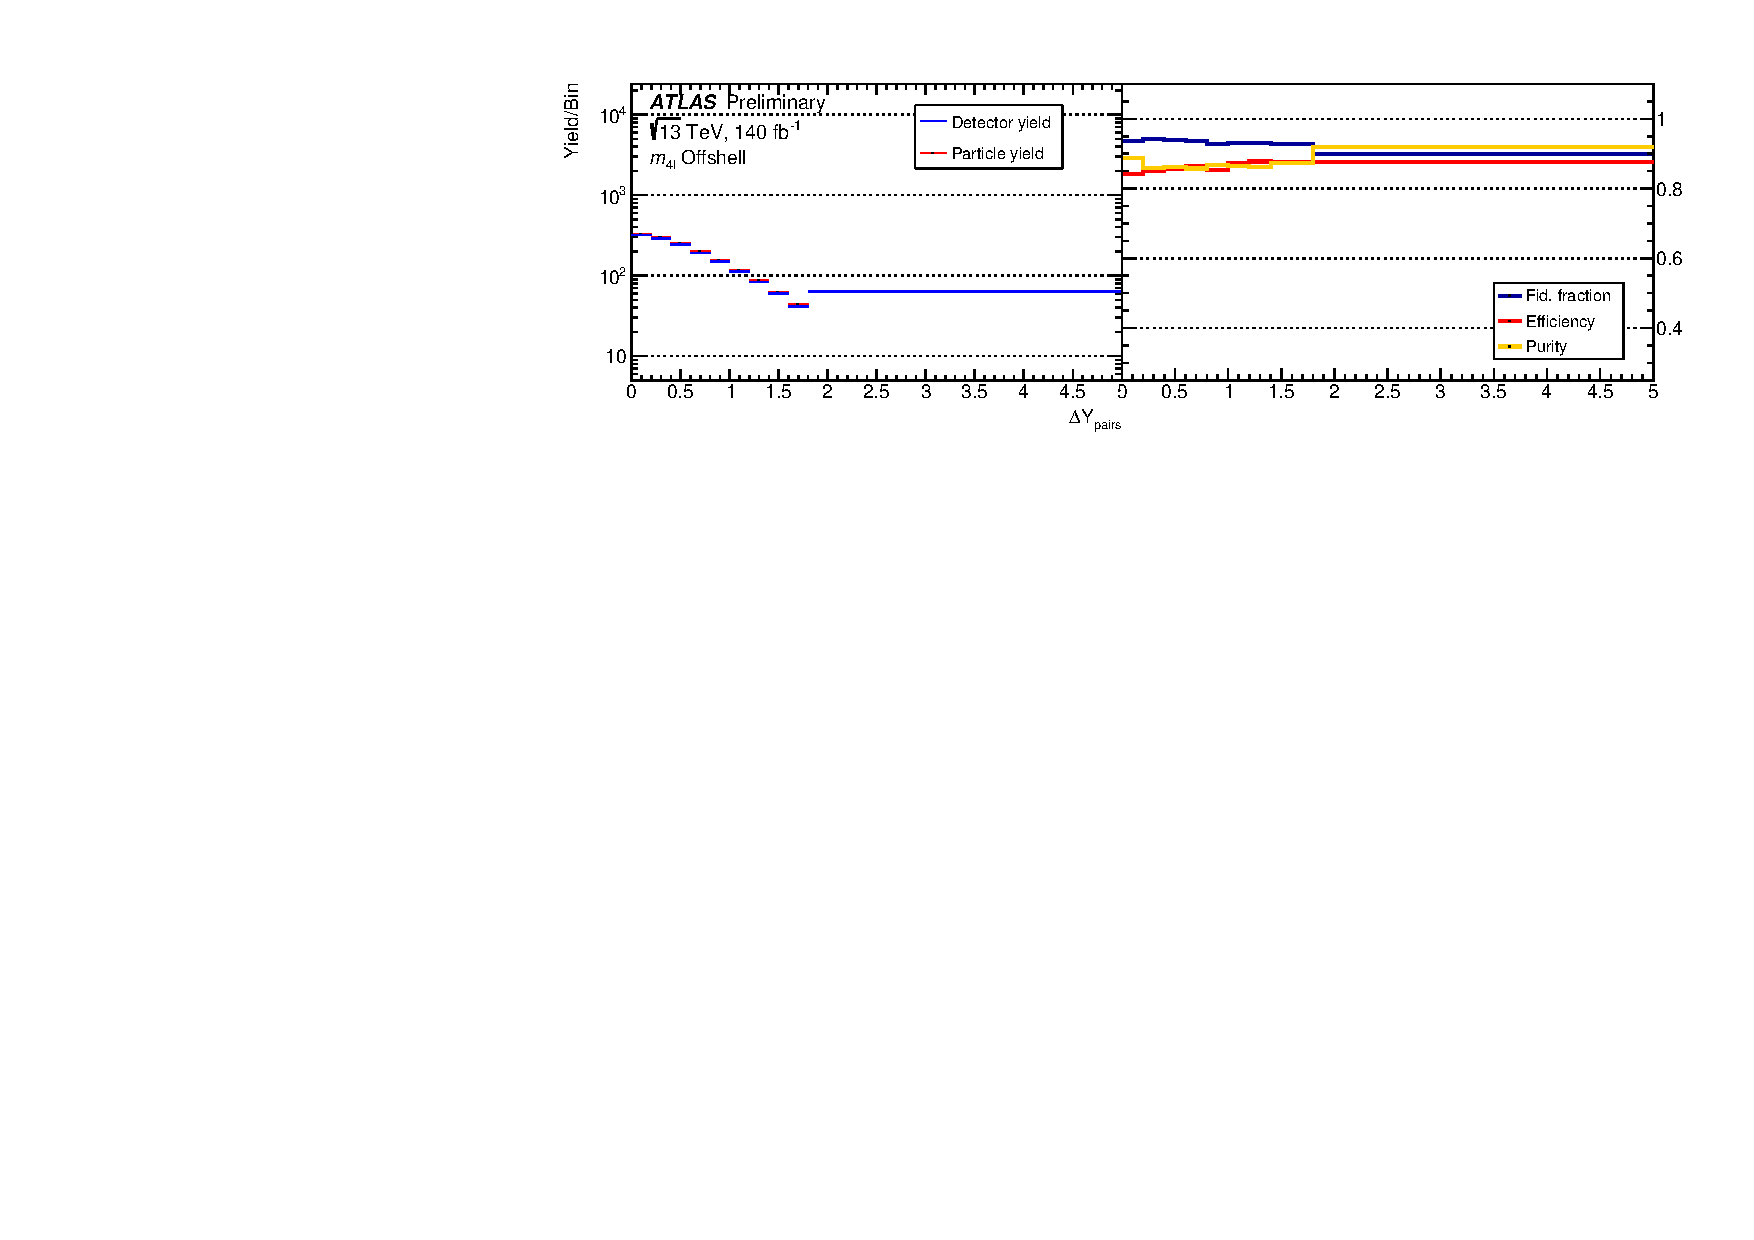
\includegraphics[width = 0.75\textwidth]{figures/UnfoldingStudies/v014_inputs/deltaYPairs_m4loffshellinputs.pdf}}\\
\caption{In the left-hand panels, the number of predicted events passing the reconstruction- and fiducial- level selections are displayed as the detector yield and particle yield, respectively. The right-hand panel shows the efficiency, fiducial purity and fiducial fraction. All variables are plotted as a function of the \dYPairs bins, in slices of the \mFourL variable which are stacked and labelled with the included \mFourL range.
  \label{fig:dypunf}}
 \end{figure}  

\FloatBarrier
\clearpage


\begin{figure}[htb]
  \centering 
  \subfigure{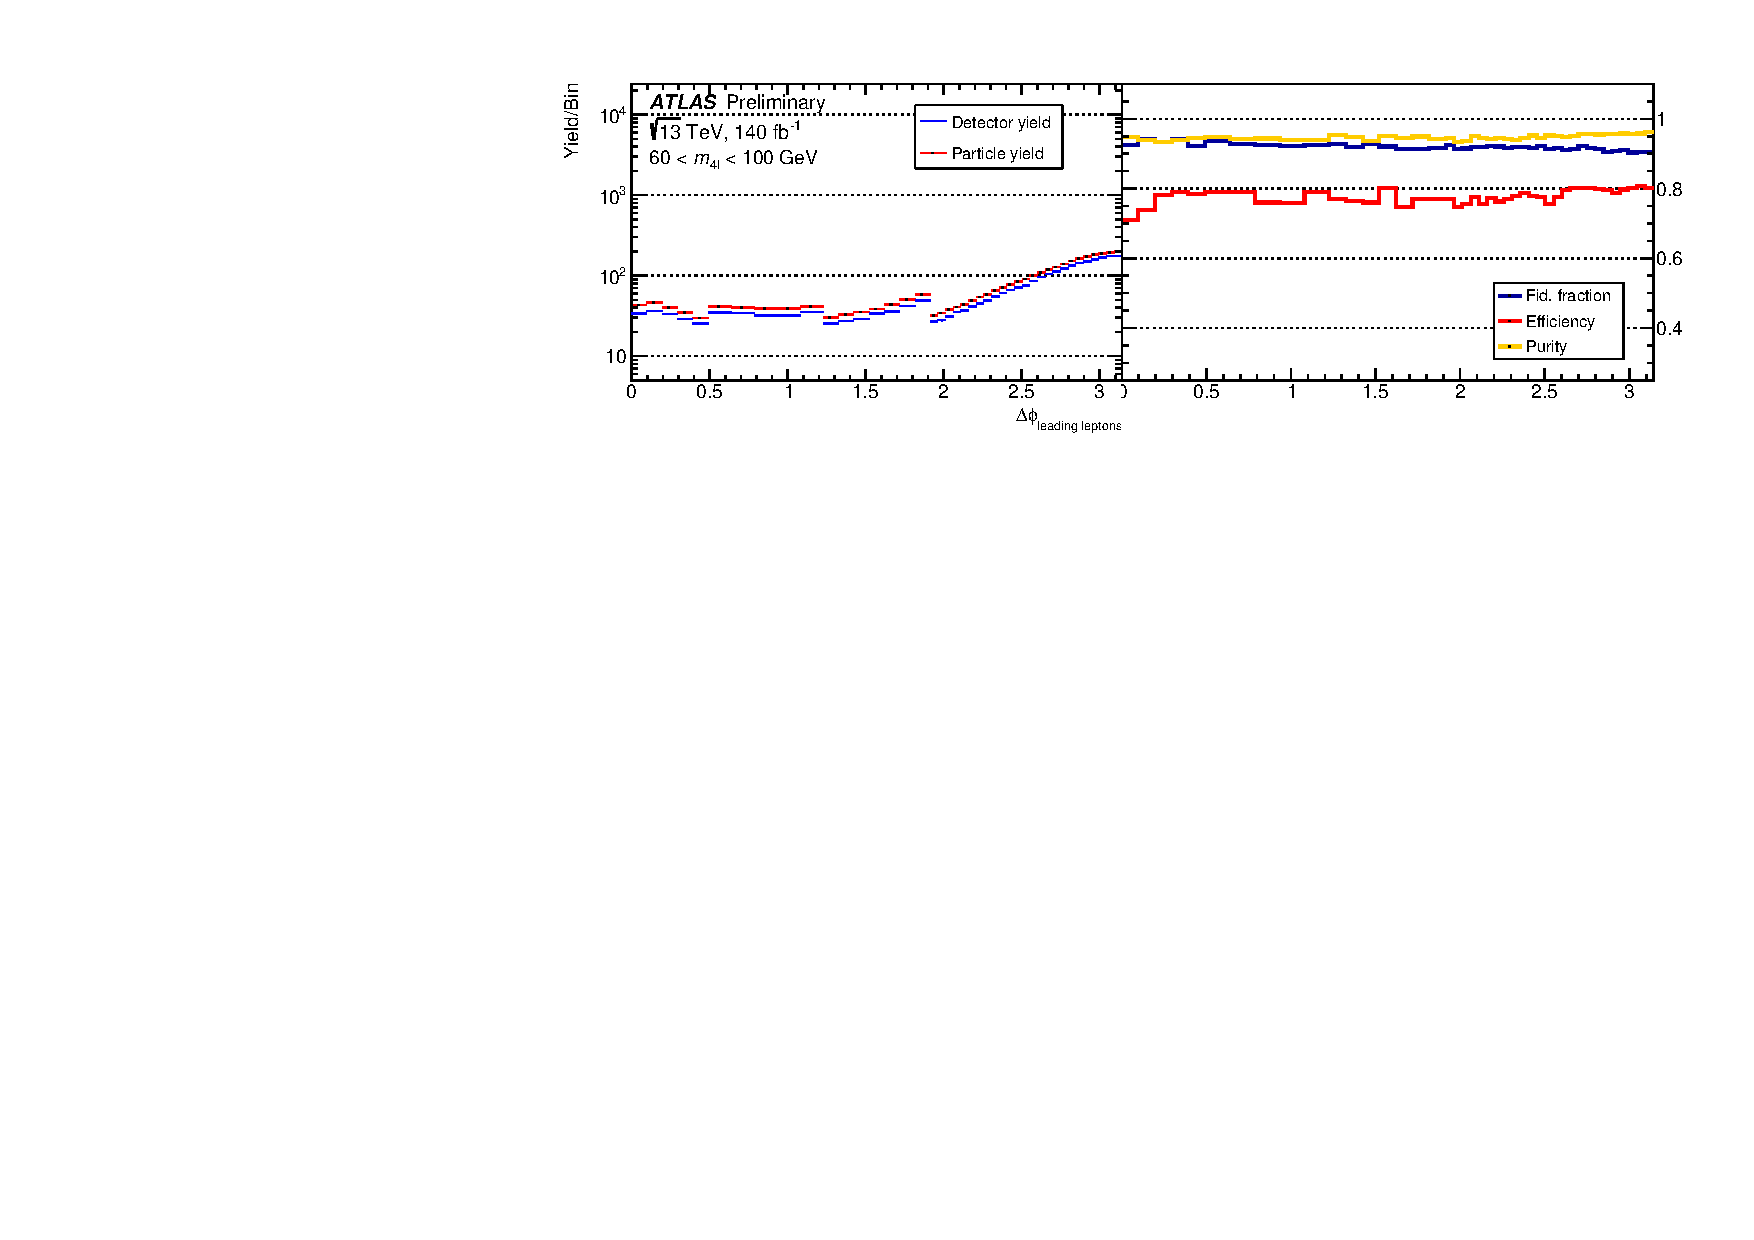
\includegraphics[width = 0.75\textwidth]{figures/UnfoldingStudies/v014_inputs/deltaPhiLeadingLeptons_m4l60-100inputs.pdf}}\\
  \subfigure{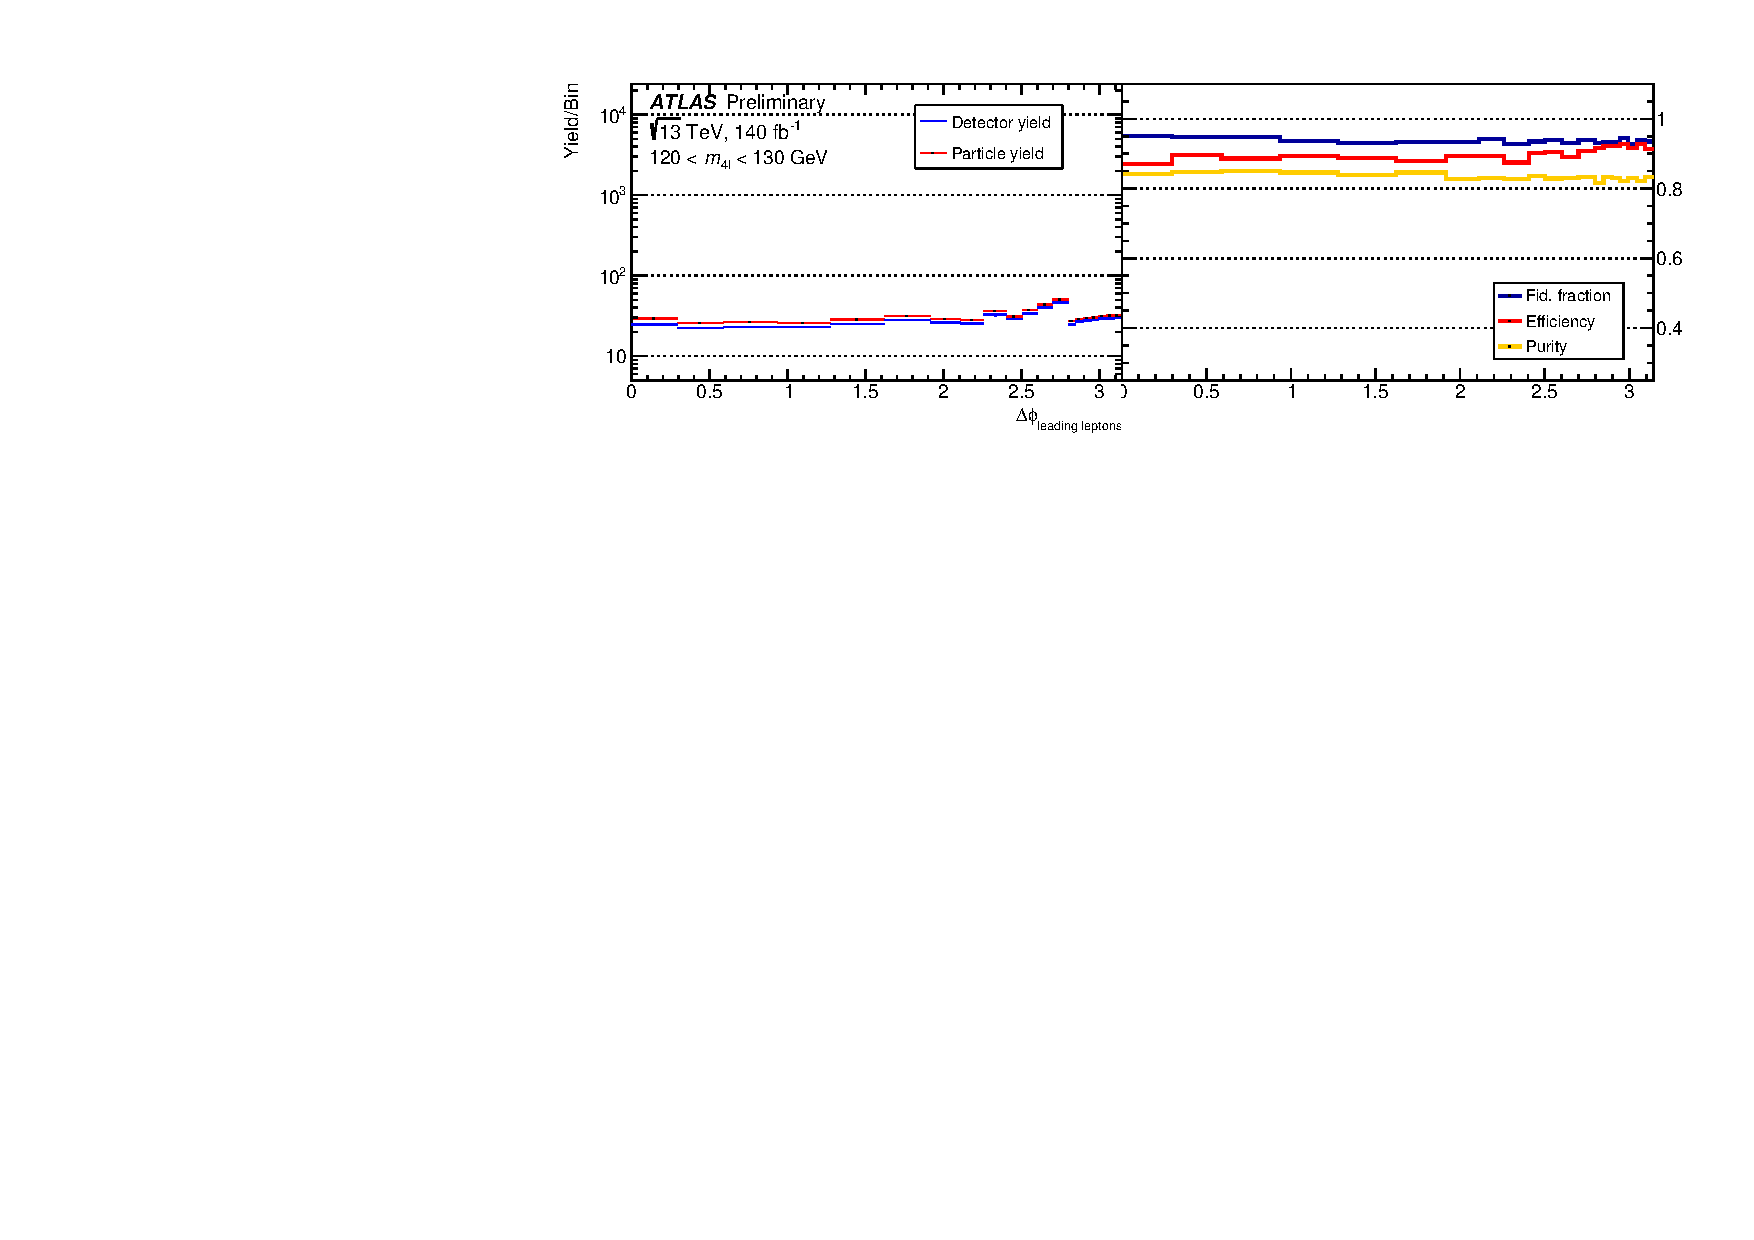
\includegraphics[width = 0.75\textwidth]{figures/UnfoldingStudies/v014_inputs/deltaPhiLeadingLeptons_m4l120-130inputs.pdf}}\\
  \subfigure{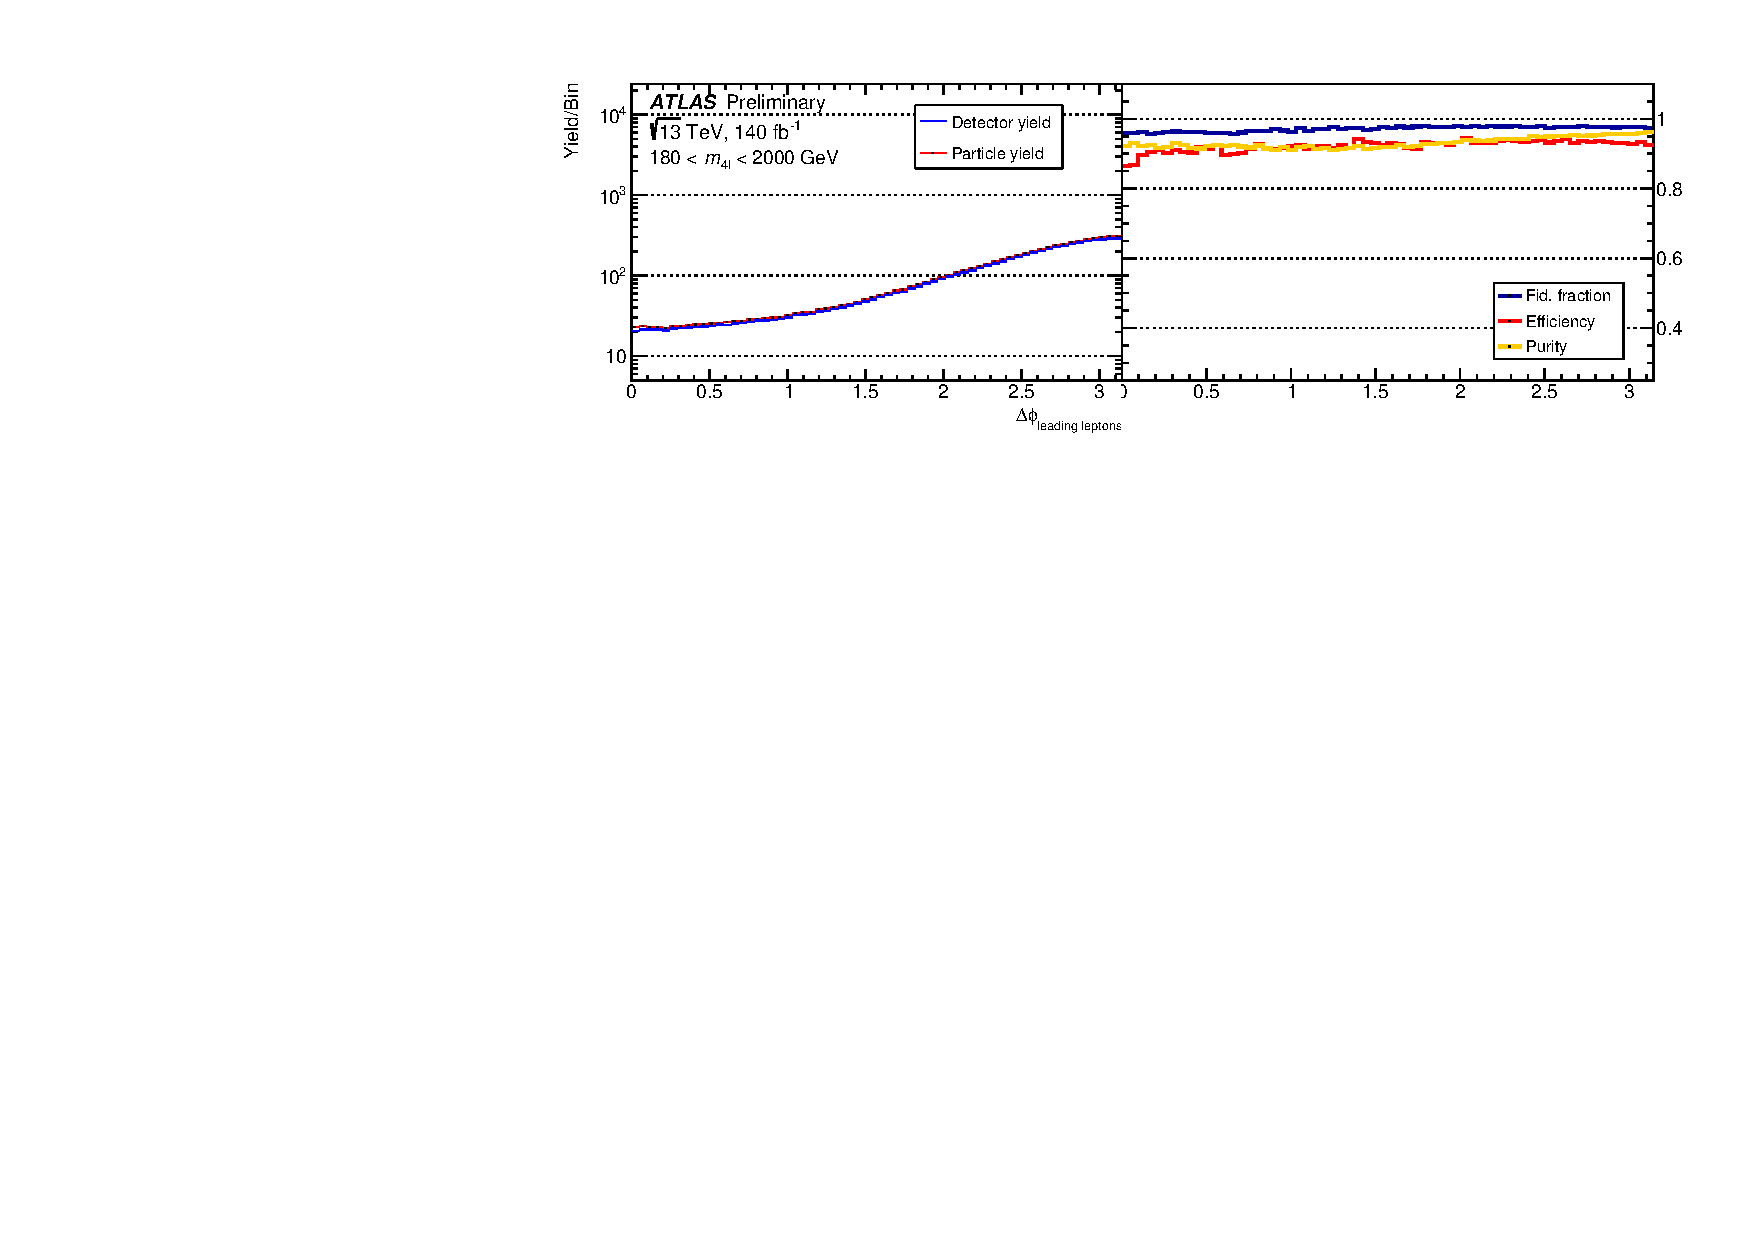
\includegraphics[width = 0.75\textwidth]{figures/UnfoldingStudies/v014_inputs/deltaPhiLeadingLeptons_m4l180-2000inputs.pdf}}\\
  \subfigure{\includegraphics[width = 0.75\textwidth]{figures/UnfoldingStudies/v014_inputs/deltaPhiLeadingLeptons_m4loffshellinputs.pdf}}\\
\caption{In the left-hand panels, the number of predicted events passing the reconstruction- and fiducial- level selections are displayed as the detector yield and particle yield, respectively. The right-hand panel shows the efficiency, fiducial purity and fiducial fraction. All variables are plotted as a function of the \dPhill bins, in slices of the \mFourL variable which are stacked and labelled with the included \mFourL range.
  \label{fig:dphiunf}}
 \end{figure}  
